\documentclass[12pt,a4paper]{report}
\usepackage{dissertation}
\makeglossaries
\makeindex

%\logo{EAAD}{School of Architecture, Art and Design}{}
%\logoB{EAAD}{School of Architecture, Art and Design}{}

%\logo{EC}{School of Sciences}{}
%\logoB{EC}{School of Sciences}{}

%\logo{ED}{Law School}{}
%\logoB{ED}{Law School}{}

\logo{EE}{School of Engineering}{}
\logoB{EE}{School of Engineering}{}

%\logo{EEG}{School of Economics and Management}{}
%\logoB{EEG}{School of Economics and Management}{}

%\logo{ELACH}{School of Letters, Arts and Human Sciences}{}
%\logoB{ELACH}{School of Letters, Arts and Human Sciences}{}

%\logo{EM}{Medical school}{}
%\logoB{EM}{Medical school}{}

%\logo{EP}{School of Psychology}{}
%\logoB{EP}{School of Psychology}{}

%\logo{ESE}{Higher School of Nursing}{}
%\logoB{ESE}{Higher School of Nursing}{}

%\logo{I3Bs}{Research Institute on Biomaterials,}{Biodegradables and Biomimetics}
%\logoB{I3Bs}{Research Institute on Biomaterials,}{Biodegradables and Biomimetics}

%\logo{ICS}{Institute of Social Sciences}{}
%\logoB{ICS}{Institute of Social Sciences}{}

%\logo{IE}{Institute of Education}{}
%\logoB{IE}{Institute of Education}{}

\author{Diogo André da Silva Esteves}

\titleA{Optimization and Standardization}
\titleB{of Medication Management Processes}
\titleC{in Hospital Environments}

\masters{Master’s Dissertation in Bioinformatics Engineering}
%\area{Area of specialization}
\supervisor{Prof. Dr. José Manuel Ferreira Machado}
\cosupervisor{Prof. Dr. Ana Regina Coelho de Sousa}

\bibpunct[,]{(}{)}{;}{a}{,}{,}
\begin{document}
\setlength{\parindent}{0em}

%-- Covers
\begin{titlepage}
\raggedright
\color{PANTONECoolGray7C}
\thelogo
\leading{20.4pt}
{\Large
\theauthor\par
\vspace{3mm}
\textbf{\thetitleA}\par
\textbf{\thetitleB}\par
\textbf{\thetitleC}
}

\vspace*{\fill}
{\footnotesize \myear}
\end{titlepage}

\null
\thispagestyle{empty}
\pagecolor{PANTONECoolGray7C}
\afterpage{\nopagecolor}
\newpage

\begin{titlepage}
\raggedright
\color{PANTONECoolGray7C}
\thelogoB
\leading{20.4pt}
{\Large
\theauthor\par
\vspace{3mm}
\textbf{\thetitleA}\par
\textbf{\thetitleB}\par
\textbf{\thetitleC}
}

\vspace{55.2mm}
\leading{16.8pt}
{\large
\themasters\par
\vspace{2mm}
\if\relax\detokenize{\thearea}\relax\else
  \thearea\par
\fi
Dissertation supervised by\par
\textbf{\thesupervisor}
\if\relax\detokenize{\thecosupervisor}\relax\else
  \par \thecosupervisor
\fi
}

\vspace*{\fill}
{\footnotesize \myear}
\end{titlepage}

%-- Document setup
\newgeometry{right=25mm, left=25mm, top=25mm, bottom=25mm}
\pagenumbering{roman}

\setlength{\parskip}{0pt}
\setlength{\parindent}{1.5em}

%-- Preamble
\chapter*{Copyright and Terms of Use for Third Party Work}
\setlength{\parskip}{1em}
\noindent
This dissertation reports on academic work that can be used by third parties as long as the internationally accepted standards and good practices are respected concerning copyright and related rights.

\noindent
This work can thereafter be used under the terms established in the license below.

\noindent
Readers needing authorization conditions not provided for in the indicated licensing should contact the author through the RepositóriUM of the University of Minho.

\section*{License granted to users of this work:}

\textit{[Caso o autor pretenda usar uma das licenças Creative Commons, deve escolher e deixar apenas um dos seguintes ícones e respetivo lettering e URL, eliminando o texto em itálico que se lhe segue. Contudo, é possível optar por outro tipo de licença, devendo, nesse caso, ser incluída a informação necessária adaptando devidamente esta minuta]}

\noindent

\includegraphics[]{images/CCBY.png}
\\
\textbf{CC BY}
\\
\url{https://creativecommons.org/licenses/by/4.0/}
\textit{[Esta licença permite que outros distribuam, remixem, adaptem e criem a partir do seu trabalho, mesmo para fins comerciais, desde que lhe atribuam o devido crédito pela criação original. É a licença mais flexível de todas as licenças disponíveis. É recomendada para maximizar a disseminação e uso dos materiais licenciados.]}

%--

\noindent

\includegraphics[]{images/CCBYSA.png}
\\
\textbf{CC BY-SA}
\\
\url{https://creativecommons.org/licenses/by-sa/4.0/}
\textit{[Esta licença permite que outros remisturem, adaptem e criem a partir do seu trabalho, mesmo para fins comerciais, desde que lhe atribuam o devido crédito e que licenciem as novas criações ao abrigo de termos idênticos. Esta licença costuma ser comparada com as licenças de software livre e de código aberto «copyleft». Todos os trabalhos novos baseados no seu terão a mesma licença, portanto quaisquer trabalhos derivados também permitirão o uso comercial. Esta é a licença usada pela Wikipédia e é recomendada para materiais que seriam beneficiados com a incorporação de conteúdos da Wikipédia e de outros projetos com licenciamento semelhante.]}

%--

\noindent

\includegraphics[]{images/CCBYND.png}
\\
\textbf{CC BY-ND}
\\
\url{https://creativecommons.org/licenses/by-nd/4.0/}
\textit{[Esta licença permite que outras pessoas usem o seu trabalho para qualquer fim, incluindo para fins comerciais. Contudo, o trabalho, na forma adaptada, não poderá ser partilhado com outras pessoas e têm que lhe ser atribuídos os devidos créditos.]}

%--

\noindent

\includegraphics[]{images/CCBYNC.png}
\\
\textbf{CC BY-NC}
\\
\url{https://creativecommons.org/licenses/by-nc/4.0/}
\textit{[Esta licença permite que outros remisturem, adaptem e criem a partir do seu trabalho para fins não comerciais, e embora os novos trabalhos tenham de lhe atribuir o devido crédito e não possam ser usados para fins comerciais, eles não têm de licenciar esses trabalhos derivados ao abrigo dos mesmos termos.]}

%--

\noindent

\includegraphics[]{images/CCBYNCSA.png}
\\
\textbf{CC BY-NC-SA}
\\
\url{https://creativecommons.org/licenses/by-nc-sa/4.0/}
\textit{[Esta licença permite que outros remisturem, adaptem e criem a partir do seu trabalho para fins não comerciais, desde que lhe atribuam a si o devido crédito e que licenciem as novas criações ao abrigo de termos idênticos.]}

%--

\noindent

\includegraphics[]{images/CCBYNCND.png}
\\
\textbf{CC BY-NC-ND}
\\
\url{https://creativecommons.org/licenses/by-nc-nd/4.0/}
\textit{[Esta é a mais restritiva das nossas seis licenças principais, só permitindo que outros façam download dos seus trabalhos e os compartilhem desde que lhe sejam atribuídos a si os devidos créditos, mas sem que possam alterá- los de nenhuma forma ou utilizá-los para fins comerciais.]}

\setlength{\parskip}{0em}
\chapter*{Acknowledgements}
\addcontentsline{toc}{chapter}{Acknowledgements}

The completion of this dissertation is the culmination of a journey that would not have been possible without the support, guidance, and collaboration of several people and institutions, to whom I wish to express my deepest gratitude.

To my supervisors, Professor José Machado (PhD), and Professor Regina Sousa (PhD), I thank you for the scientific guidance, methodological rigor, and constant encouragement. Professor José Machado's vast experience in health information systems and Professor Regina Sousa's insightful technical contributions on software architecture were fundamental pillars for the realization of this project.

I would like to express my sincere gratitude to Professor António Abelha (PhD) and Rui Miranda (PhD student). Professor Abelha’s guidance in the clinical context and his mastery of data analysis were crucial for understanding the complex processes of hospital medication management. 

Rui Miranda was especially helpful in the initial stages of my learning in the hospital environment, facilitating my integration into the systems and, above all, teaching me how to program and debug in TypeScript/React knowledge that proved essential for the development of this artefact.

To the University of Minho and its School of Engineering, I am grateful for the conditions and resources provided, which were essential for the development of this research.

My gratitude extends to the administration and healthcare professionals of the Hospital da Misericórdia de Vila Verde (SCMVV). Their availability and the sharing of practical knowledge on hospital management and the systems in production were invaluable. Special thanks are due to the SCMVV's information systems technicians for their assistance and for providing the access that allowed a detailed analysis of the legacy systems.

To my colleagues from the Master's in Bioinformatics Engineering, I thank you for the camaraderie, the enriching discussions, and the knowledge sharing that so greatly contributed to my academic growth.

Finally, to my family, a heartfelt thank you for the unconditional support, patience, and constant encouragement, which were my safe harbor throughout this journey.

To everyone, my sincerest thanks.

\cleardoublepage 
\chapter*{Statement of Integrity}
\setlength{\parskip}{1em}
\noindent
I hereby declare having conducted this academic work with integrity.

\noindent
I confirm that I have not used plagiarism or any form of undue use of information or falsification of results along the process leading to its elaboration.

\noindent
I further declare that I have fully acknowledged the Code of Ethical Conduct of the University of Minho.

\phantom{space}

\noindent
University of Minho, Braga, \myear

\vspace{25mm}
\noindent\theauthor
\setlength{\parskip}{0em}
\chapter*{Resumo}
\addcontentsline{toc}{chapter}{Resumo}

A fragmentação dos sistemas de informação no Serviço Nacional de Saúde português representa um desafio sistémico à segurança do doente e à eficiência operacional, particularmente no ciclo do medicamento. Este projeto de dissertação propõe-se a endereçar este problema no contexto da Santa Casa da Misericórdia de Vila Verde (SCMVV) através do desenho, desenvolvimento e avaliação de uma plataforma de software centralizada. O objetivo é unificar os fluxos de trabalho clínico-farmacêuticos, atualmente dispersos por múltiplos sistemas legados, numa única interface de utilizador moderna e coesa.

Adotando uma metodologia de \textit{Design Science Research} (DSR), o projeto irá criar um artefacto tecnológico — um sistema web com uma arquitetura de microsserviços (Node.js) e um frontend reativo (TypeScript/React) — concebido para se integrar com a infraestrutura existente. A avaliação do sistema será focada em indicadores de desempenho chave (KPIs) específicos, antecipando-se uma redução significativa dos erros de medicação e um aumento da eficiência dos processos para enfermeiros e farmacêuticos. A contribuição principal deste trabalho será a validação de um modelo de modernização sociotécnica que, se bem-sucedido, poderá servir de referência para outras unidades de saúde que enfrentam desafios de fragmentação semelhantes.

\vspace{6mm}
\noindent\textbf{Palavras-chave:} Sistemas de Informação em Saúde, Segurança do Doente, Gestão da Medicação, Design Science Research, Unificação de Sistemas, Interoperabilidade Clínica.

\vspace*{\fill}

\selectlanguage{english}
\chapter*{Abstract}
\addcontentsline{toc}{chapter}{Abstract}

\begingroup
\emergencystretch=2em
\sloppy
The fragmentation of information systems within the Portuguese National Health Service constitutes a systemic challenge to patient safety and operational efficiency, particularly in the medication management lifecycle. This dissertation project aims to address this problem in the context of the Santa Casa da Misericórdia de Vila Verde (SCMVV) by designing, developing, and evaluating a centralized software platform. The primary objective is to unify the clinical-pharmaceutical workflows, currently fragmented across multiple legacy systems, into a single, modern, and cohesive user interface.

Adopting a \textit{Design Science Research} (DSR) methodology, the project will create a technological artifact---a web-based system featuring a microservices architecture (Node.js) and a reactive frontend (TypeScript/\-React)---designed to integrate with the existing infrastructure. The system's evaluation will focus on specific Key Performance Indicators (KPIs), with the anticipation of achieving a significant reduction in medication errors and an increase in process efficiency for nurses and pharmacists. The main contribution of this work will be the validation of a socio\-technical modernization model that, if successful, could serve as a reference for other healthcare institutions facing similar fragmentation challenges.

\vspace{6mm}
\noindent\textbf{Keywords:} Health Information Systems,\allowbreak Patient Safety,\allowbreak Medication Management,\allowbreak Design Science Research,\allowbreak System Unification,\allowbreak Clinical Interoperability.
\endgroup 

%-- Glossary definitions
% Glossary and acronyms definitions (minimal set)
\newacronym{scmvv}{SCMVV}{Santa Casa da Misericórdia de Vila Verde}
\newacronym{cdss}{CDSS}{Clinical Decision Support System}
\newacronym{his}{HIS}{Hospital Information System}
\newacronym{hit}{HIT}{Health Information Technology}
\newacronym{dsr}{DSR}{Design Science Research}
\newacronym{hl7}{HL7}{Health Level Seven}
\newacronym{fhir}{FHIR}{Fast Healthcare Interoperability Resources}
\newacronym{api}{API}{Application Programming Interface}
\newacronym{jwt}{JWT}{JSON Web Token}
\newacronym{ldap}{LDAP}{Lightweight Directory Access Protocol}
\newacronym{uat}{UAT}{User Acceptance Testing}
\newacronym{gdpr}{GDPR}{General Data Protection Regulation}
\newacronym{ddi}{DDI}{Drug-Drug Interaction}
\newacronym{ui}{UI}{User Interface}
\newacronym{roi}{ROI}{Return on Investment}
\newacronym{ehr}{EHR}{Electronic Health Record}
\newacronym{sso}{SSO}{Single Sign-On}
\newacronym{srs}{SRS}{Software Requirements Specification}
\newacronym{sus}{SUS}{System Usability Scale}
\newacronym{wcag}{WCAG}{Web Content Accessibility Guidelines}
\newacronym{eda}{EDA}{Event-Driven Architecture}
\newacronym{aida}{AIDA-PCE}{Aplicação Integrada para a Área da Saúde - Prescrição, Codificação e Executável}
\newacronym{pem}{PEM}{Prescrição Eletrónica Médica}
\newacronym{adse}{ADSE}{Assistência na Doença aos Servidores do Estado}
\newacronym{sonho}{SONHO}{Sistema de Informação Hospitalar (Portugal)}
\newacronym{emar}{eMAR}{Electronic Medication Administration Record}
\newacronym{bcma}{BCMA}{Barcode Medication Administration}
\newacronym{sns}{SNS}{Serviço Nacional de Saúde}
\newacronym{spms}{SPMS}{Serviços Partilhados do Ministério da Saúde}
\newacronym{sclinico}{SClínico}{SClínico}

% Glossary entries (non-acronyms)
\newglossaryentry{apigateway}{name={API Gateway}, description={A server that acts as a single entry point for API requests, responsible for request routing, composition, and protocol translation}}
\newglossaryentry{servicemesh}{name={Service Mesh}, description={An infrastructure layer for managing service-to-service communication in a microservices architecture, providing features like traffic management, security, and observability}}
\newglossaryentry{cqrs}{name={CQRS}, description={Command Query Responsibility Segregation; a pattern that separates read and write operations for better scalability and maintainability}}


\phantomsection
\tableofcontents

\cleardoublepage
\listoffigures

% List of tables
\renewcommand*{\listtablename}{List of Tables}
\listoftables
\clearpage

% Acronyms
\printglossary[type=\acronymtype,nonumberlist, title={Acronyms}]

% Glossary
\printglossary[title={Glossary}, nonumberlist]

\cleardoublepage
\pagenumbering{arabic}

%-- Dissertation 
\part{Introductory material}

\chapter{Introduction}

\section{Context and Problem Definition}

Medication management is a high-stakes, complex process central to modern healthcare delivery. Its successful execution is critical for patient safety, yet it remains a major source of preventable adverse events. The landmark report "To Err is Human" by the Institute of Medicine brought global attention to the prevalence of medical errors, identifying them as a leading cause of morbidity and mortality \cite{kohn2000}. Subsequent research and initiatives by the World Health Organization have reinforced this reality, indicating that medication-related harm affects one in ten patients globally and that the associated costs are substantial \cite{who2017, who2022}.

A primary contributing factor to this problem is the fragmented nature of Health Information Technology (\gls{hit}) ecosystems within hospitals \cite{berwick2008}. Many healthcare institutions operate on a patchwork of legacy systems, often developed decades apart using disparate technologies \cite{kazemi2016}. This technological heterogeneity creates significant barriers to interoperability, resulting in information silos where critical patient data is not shared effectively between departments or professionals. This fragmentation directly undermines continuity of care and has been identified as a key threat to patient safety \cite{ash2004, keasberry2017}. The workflow, which should be a seamless continuum from a physician's prescription to pharmaceutical validation and finally to nursing administration, is often interrupted by manual processes, verbal communications, and data re-entry, each step introducing a new opportunity for error.

\begin{figure}[htbp]
    \centering
    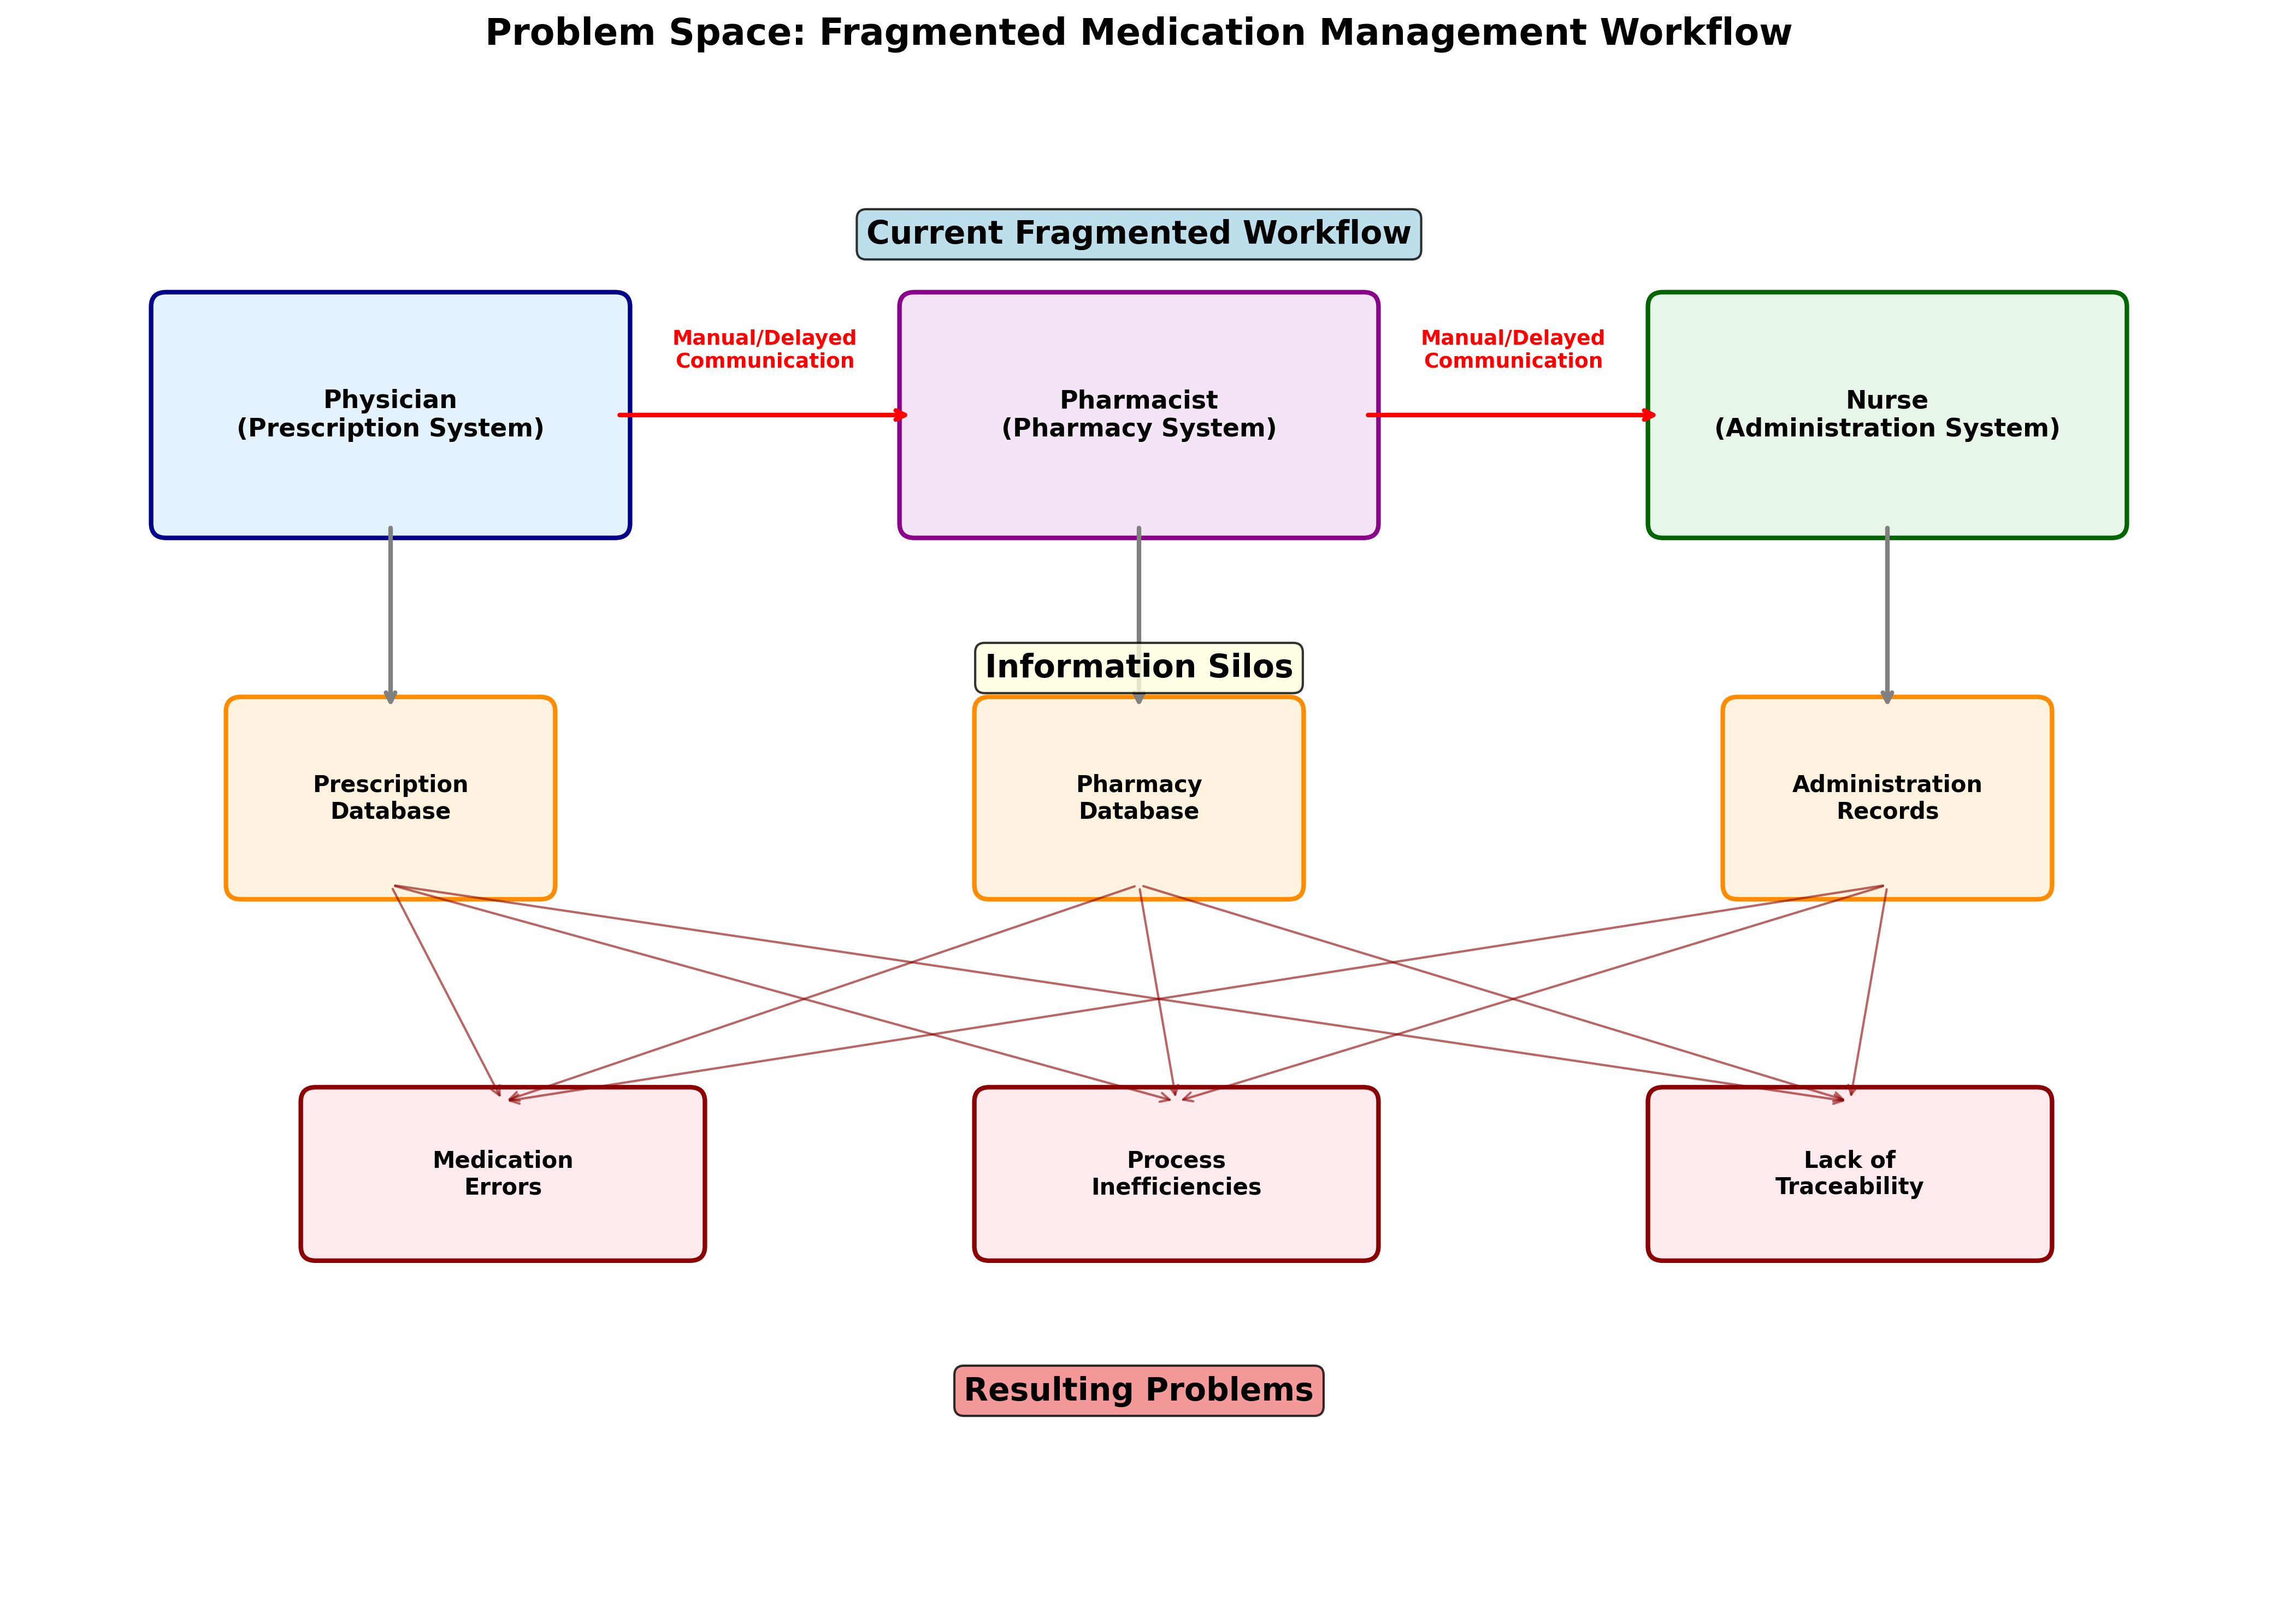
\includegraphics[width=0.9\textwidth]{images/generated/problem_space_diagram.png}
    \caption{Conceptual diagram of the problem space, illustrating the fragmented communication flow and resulting information silos that contribute to medication errors and operational inefficiencies.}
    \label{fig:problem_space}
\end{figure}

The Santa Casa da Misericórdia de Vila Verde (\gls{scmvv}) serves as a representative case study for these systemic challenges. Its core operations rely on the \gls{aida}, a legacy system with significant limitations, including a non-intuitive interface, a lack of real-time clinical decision support (e.g., for drug interactions), and poor integration capabilities \cite{moss2015, bowles2020}. This environment compromises patient safety and hampers operational efficiency. This dissertation addresses these issues by detailing the design, development, and implementation of a modern, integrated medication management system aimed at creating a cohesive, safe, and efficient clinical workflow.

\section{Objectives and Dissertation Structure}

The primary goal of this research is to develop and evaluate an integrated medication management system that optimizes the prescription, validation, dispensing, and administration processes at the SCMVV, thereby enhancing patient safety and operational efficiency. To achieve this, a set of specific scientific and technological objectives was defined. Scientifically, the aim was to analyze the system's impact on medication error rates, evaluate its effect on clinical workflow efficiency, and assess its usability and acceptance among clinical staff. Technologically, the objectives were to design a scalable microservices architecture, develop a robust clinical decision support engine, create an intuitive user interface using modern web technologies, ensure seamless integration with legacy systems, and establish a comprehensive audit trail for all medication-related activities \cite{belle2013, misra2023, mandl2020, european2016}.

This dissertation is organized to logically present the research journey. Following this introduction, Chapter 2 provides a comprehensive review of the State of the Art, including point-of-care administration (eMAR/BCMA) and process standardization in healthcare (Sections~\ref{sec:emar_bcma} and~\ref{sec:process_standardization}), as well as the national context (Section~\ref{sec:national_context_portugal}). Chapter 3 outlines the Work Plan, detailing the project's timeline and phases. Chapter 4 describes the in-depth research Methodology, including the architectural choices and evaluation strategies. Chapter 5 details the Expected Results and Evaluation Plan. Chapter 6 presents Results obtained to date. Chapter 7 offers a Discussion of these results, contextualizing them within the broader literature. Finally, Chapter 8 provides the Conclusion and Future Work, summarizing the contributions and proposing directions ahead. 

\section{Current Context at SCMVV}
\label{sec:context_scmvv}

To address identified gaps in the contextualization of the case study, this section documents the current medication-management processes and supporting information systems at the Santa Casa da Misericórdia de Vila Verde (\gls{scmvv}). The intent is to provide a concrete baseline that motivates the proposed solution and frames subsequent evaluation.

\begin{itemize}
    \item Systems in use and their roles (e.g., \gls{aida}\,/AIDA-PCE; possible interactions with hospital HIS such as SONHO; national platforms such as \gls{pem}), within the scope of medication management.
    \item End-to-end workflow as practiced today: physician prescription, pharmaceutical validation, stock/dispensing, and nursing administration, highlighting where manual steps or data re-entry occur.
    \item Known integration gaps and failure points affecting continuity of care (e.g., absence of real-time decision support or cross-module synchronization).
    \item Baseline indicators to be captured where available (e.g., error types, volumes of movements for controlled substances, turnaround times), to support before/after reasoning.
\end{itemize}

\section{As-is System Architecture (SCMVV)}
\label{sec:as_is_architecture}

This section outlines a high-level description of the current (as-is) technical architecture supporting medication management at \gls{scmvv}, to contrast later with the target architecture. The description will enumerate principal modules, databases, interfaces, and data flows relevant to prescription, validation, dispensing, and administration, and will explicitly indicate where interfaces or interoperability are absent or manual.

\section{Current Medication Process Organization at SCMVV}
\label{sec:current_process_org}

This section documents the organizational perspective of the medication process at \gls{scmvv}, complementing the technical as-is view. It focuses on roles, handoffs, and standard operating procedures as practiced today, highlighting opportunities for standardization.

\begin{itemize}
    \item Roles and responsibilities across disciplines: prescribing physicians, hospital pharmacists (validation and stock management), and nursing staff (administration and recording).
    \item Artefacts (main actual artefact is a legacy artefact in a vb.net project (AIDA-PCE)) and records in use (systems and/or paper forms) at each stage, and where transcriptions or verbal confirmations occur.
    \item Typical handoffs between departments, including triggers (e.g., a prescription becomes available for validation) and feedback loops.
    \item Known variability across wards/services and its impact on consistency and safety.
    \item Pointers to figures/diagrams: process flow diagram of the current cycle; swimlane diagram of cross-role interactions; inventory of current forms/screens.
\end{itemize}

\begin{figure}[htbp]
    \centering
    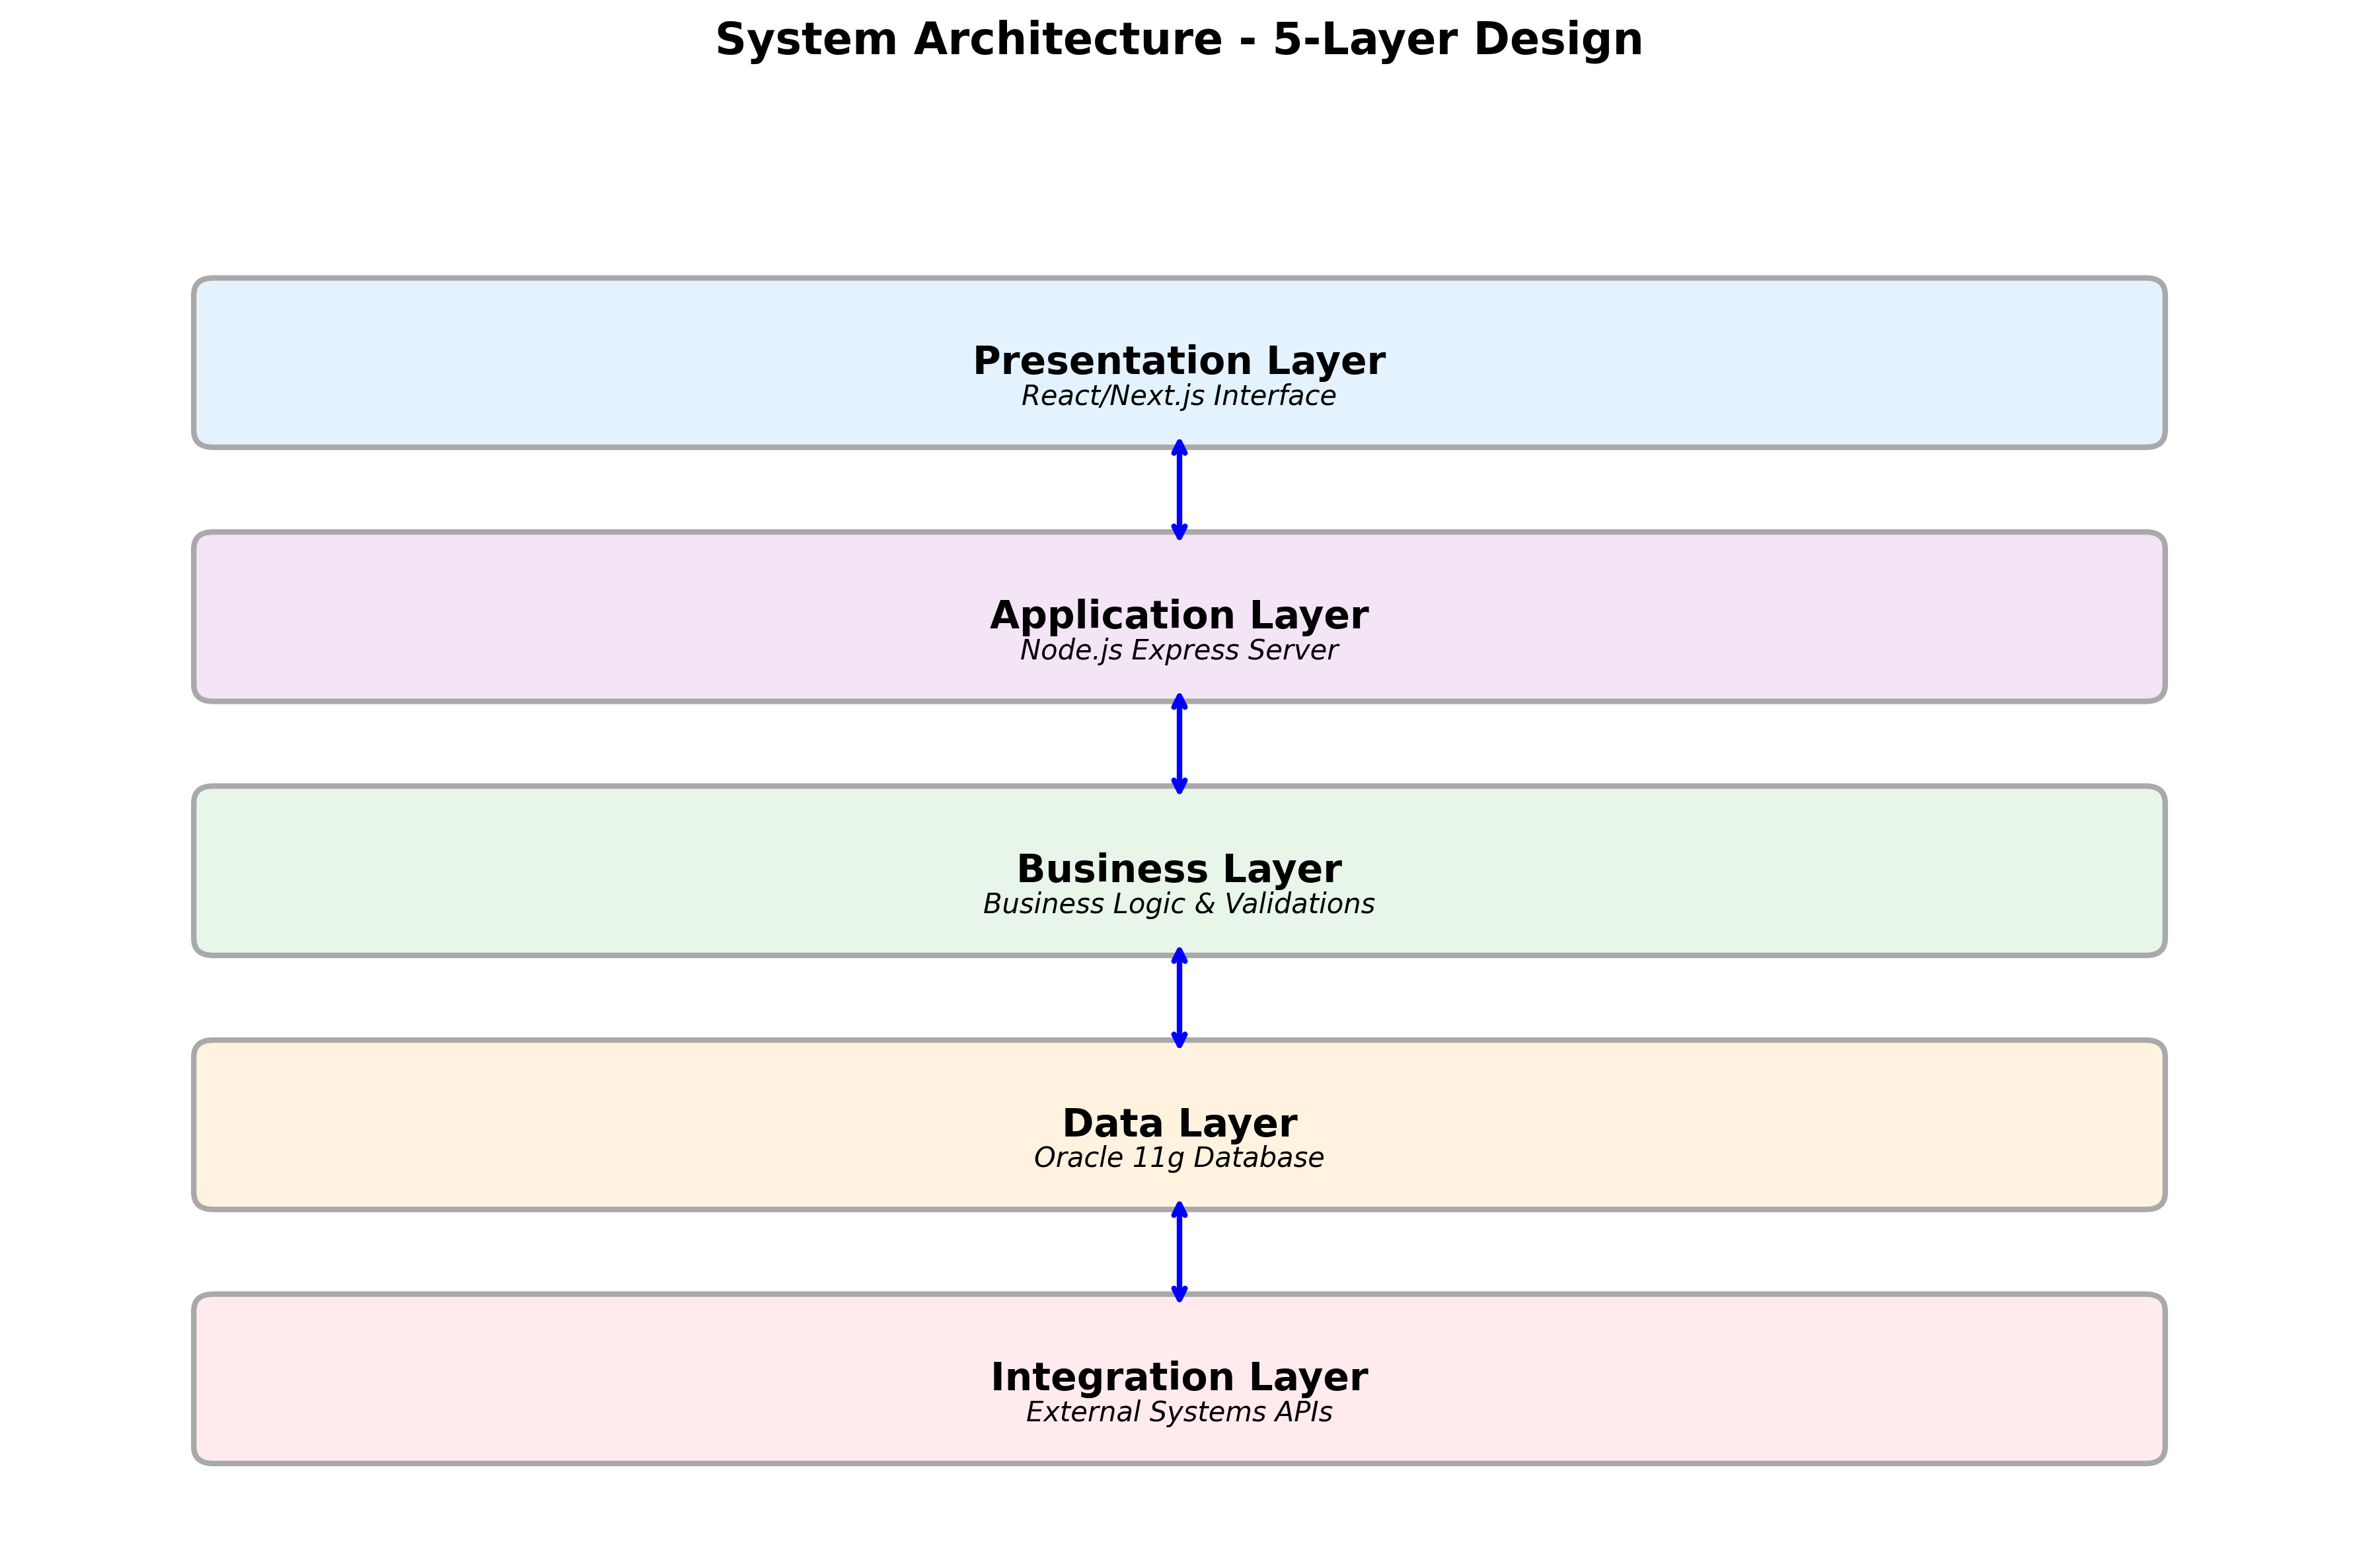
\includegraphics[width=0.95\textwidth]{images/generated/system_architecture.png}
    \caption{Placeholder: As-is architecture overview at SCMVV (to be replaced with a specific as-is diagram). Source: consolidated from institutional documents (docs/) and AI-generated analyses (tmp\_ai\_reports/). Elements to include: core legacy systems (e.g., AIDA-PCE), supporting HIS modules, databases, interfaces/APIs (if any), manual/CSV exchanges, authentication/identity context, and known failure points.}
    \label{fig:as_is_architecture_scmvv}
\end{figure}

\begin{figure}[htbp]
    \centering
    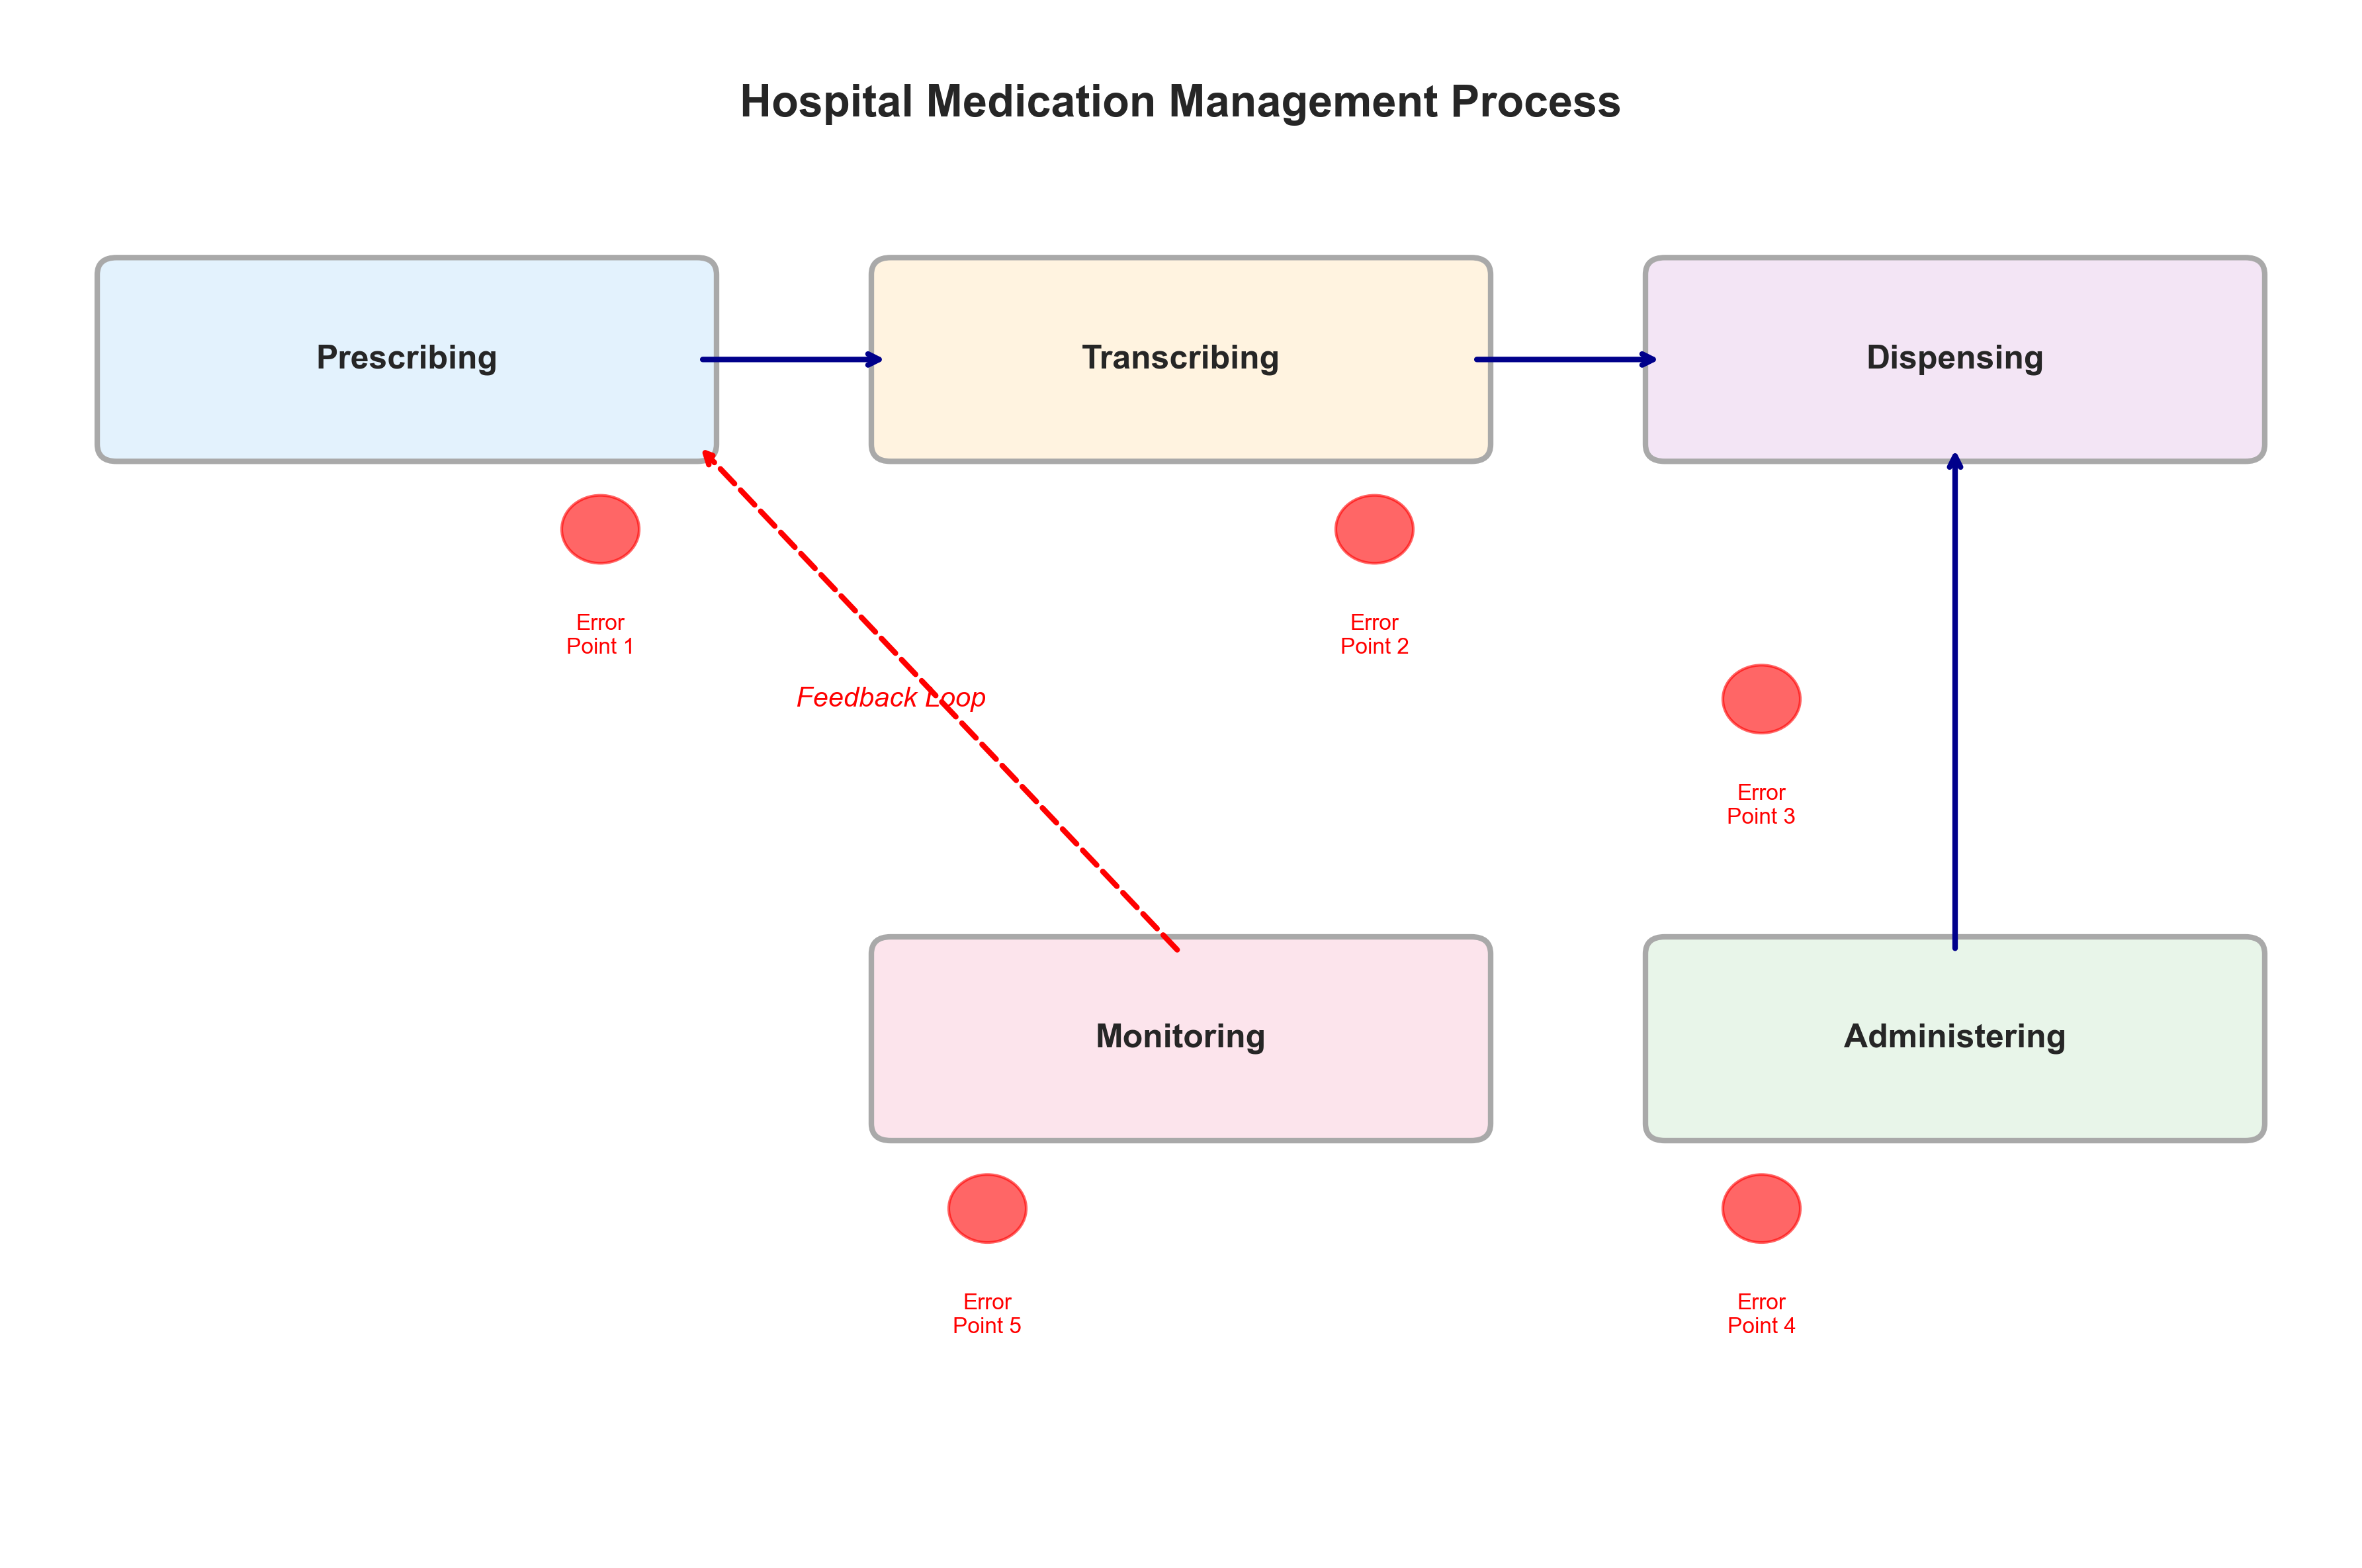
\includegraphics[width=0.95\textwidth]{images/generated/medication_flow_process.png}
    \caption{Placeholder: Current medication process swimlane (to be replaced with a specific SCMVV swimlane). Source: consolidated from institutional documents (docs/) and AI-generated analyses (tmp\_ai\_reports/). Lanes to include: Physician (prescription), Pharmacy (validation and stock), Nursing (administration/recording), and Systems/Records (AIDA-PCE, other records or paper). Mark handoffs, feedback loops, and points of transcription.}
    \label{fig:as_is_swimlane_scmvv}
\end{figure}
\chapter{State of the Art}

\section{Hospital Medication Management Systems}

Medication management is a cornerstone of patient safety in hospital environments. The increasing complexity of prescriptions, coupled with the risk of drug interactions, compels healthcare systems to operate with maximum efficiency and safety. In recent years, various solutions have been developed to automate parts of this process, from prescription to administration. However, the lack of integration between these systems—particularly among physicians, pharmacies, and nurses—continues to pose risks and inefficiencies \cite{bowles2020, kallio2020}. This work proposes a solution that addresses these gaps by focusing on backend integration and the automation of hospital processes, using technologies like Java and Node.js to standardize and optimize medication management \cite{Ghobadi2022}.

\subsection{Historical Evolution}

Hospital Information Systems (HIS) have evolved significantly from the early mainframe-based systems of the 1960s. The transition to departmental systems in the 1980s and their subsequent integration via Health Level Seven (HL7) \cite{dolin2006, mandl2020} in the 1990s laid the groundwork for modern systems.

\begin{figure}[htbp]
    \centering
    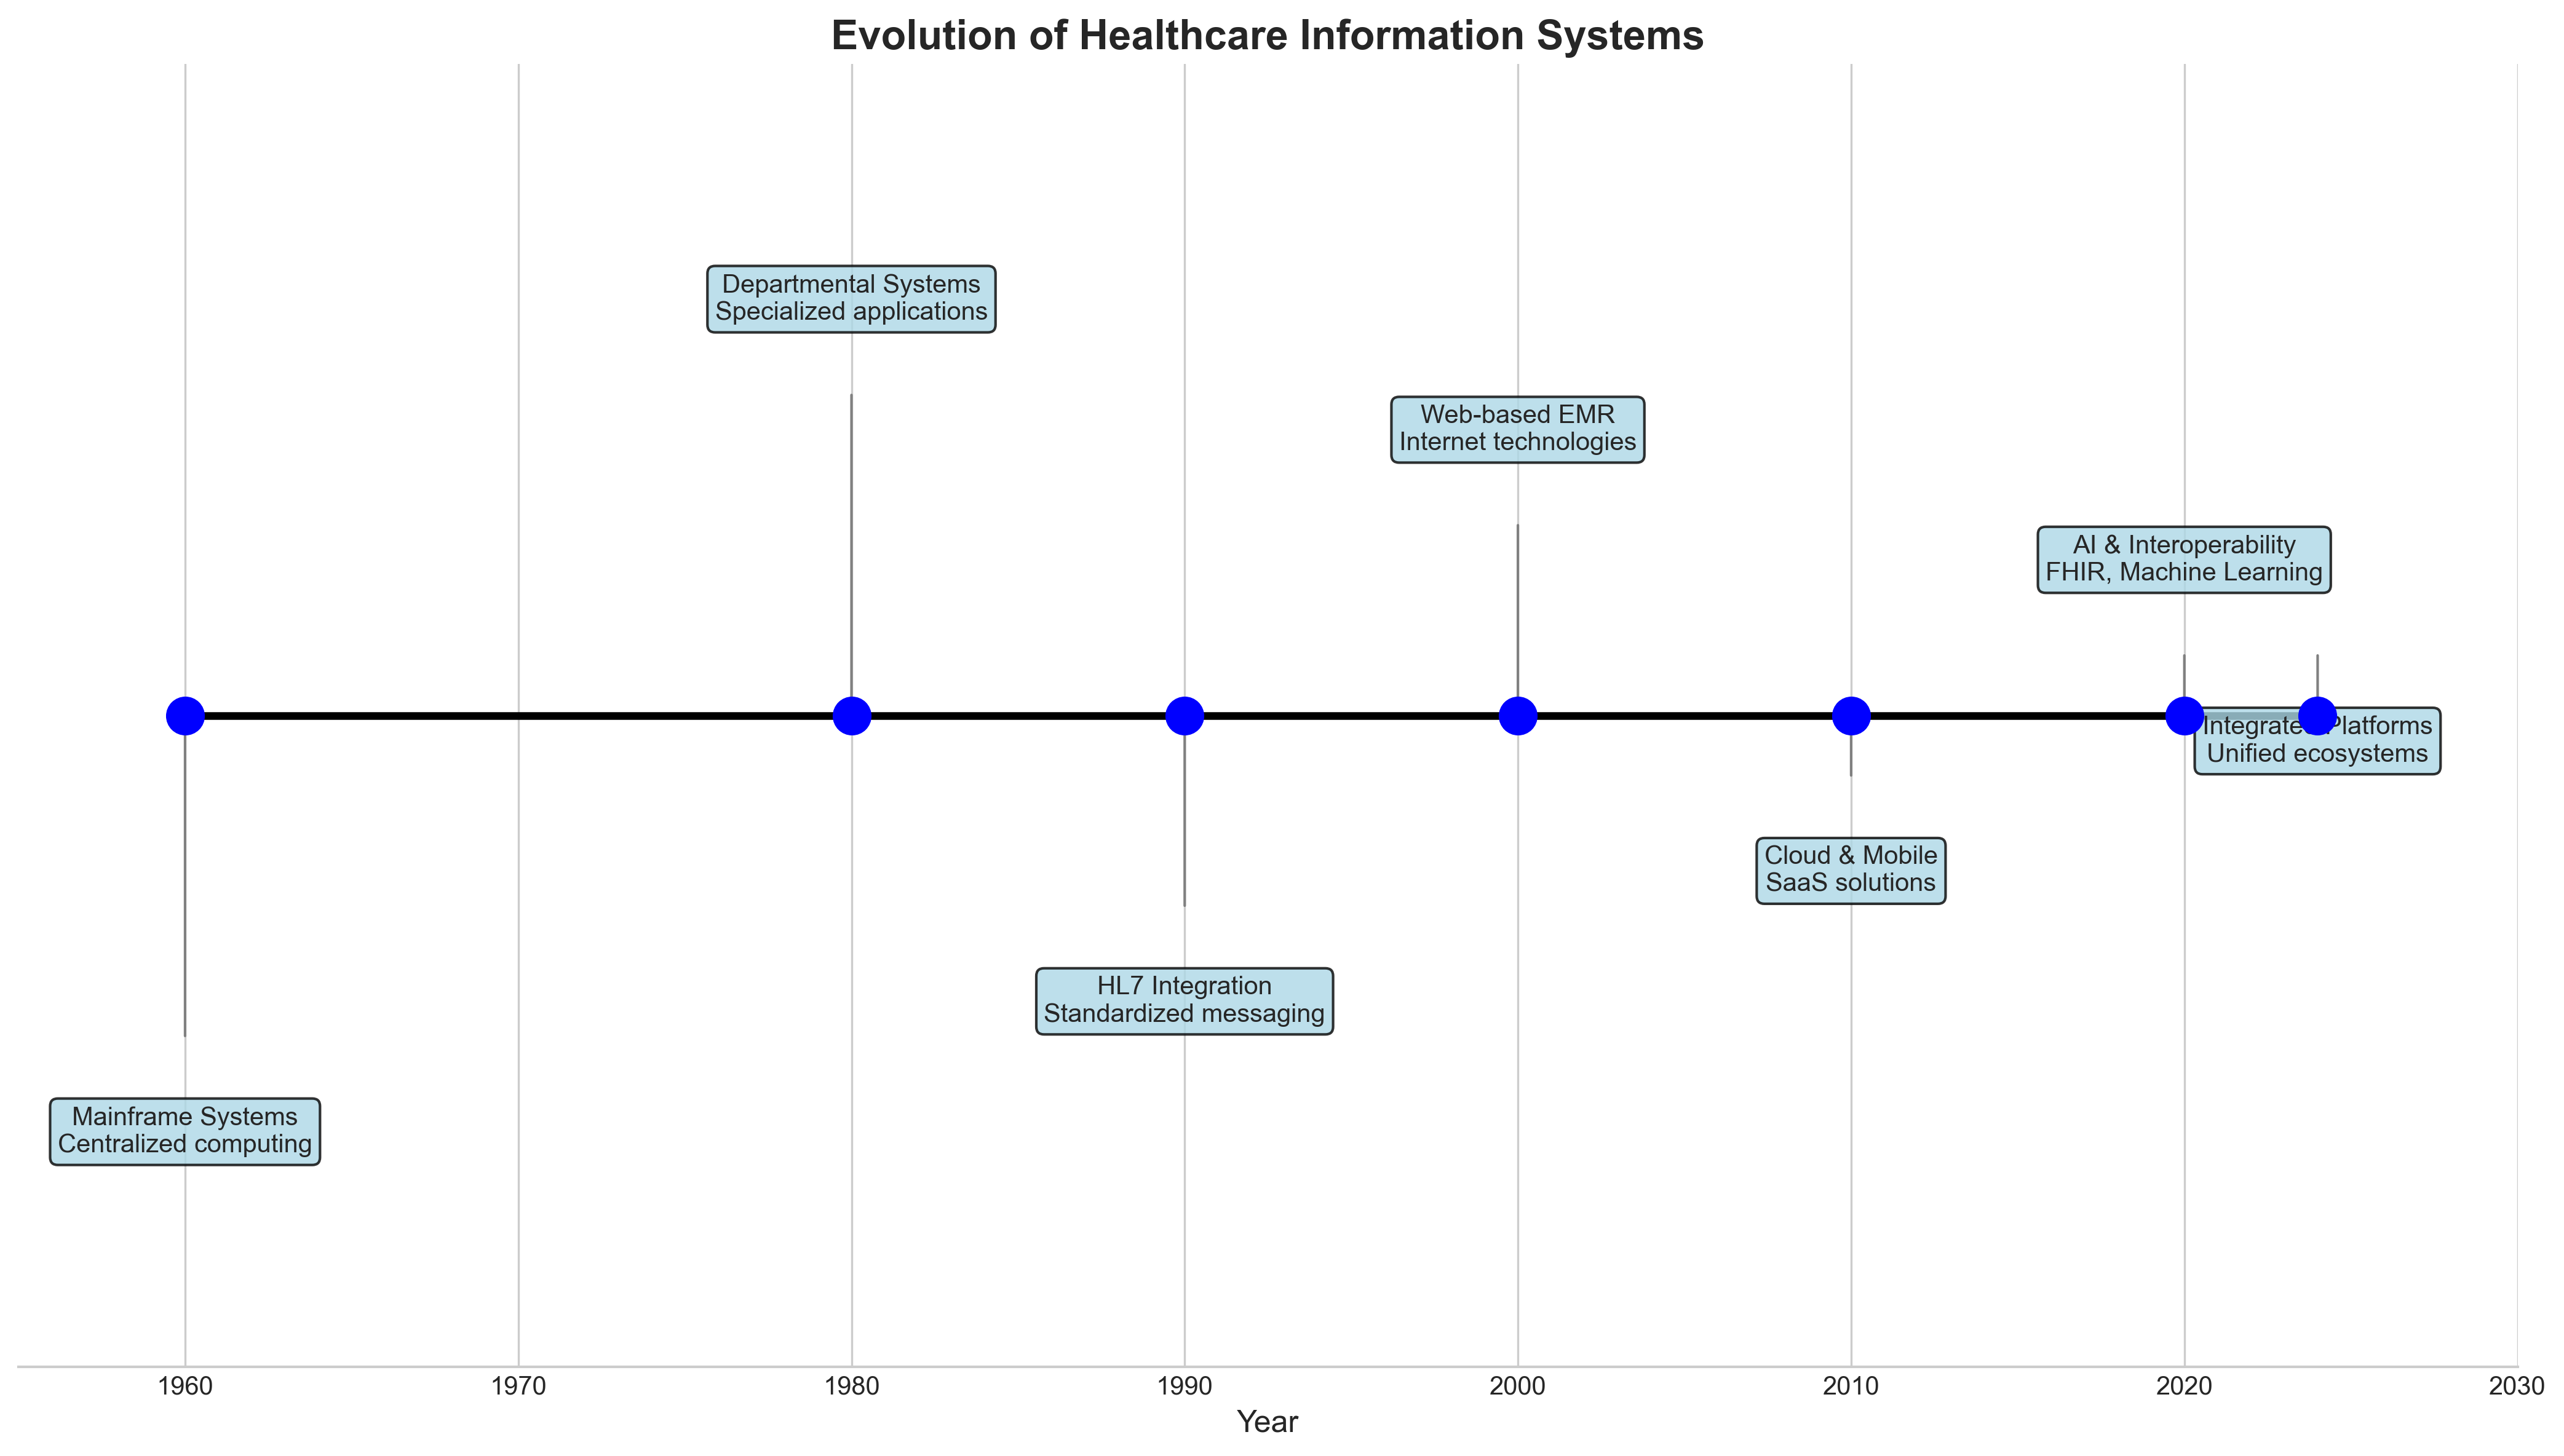
\includegraphics[width=0.95\textwidth]{images/generated/healthcare_it_timeline.png}
    \caption{Evolution of healthcare information systems from mainframe to integrated platforms \citep{shermock2023, vaghasiya2023}.}
    \label{fig:healthcare_it_timeline}
\end{figure}

\subsection{Current Commercial Systems}

The current landscape of commercial hospital management systems is dominated by a few key vendors. Epic Systems \cite{hertzum2022} has established itself as a market leader in the United States with its EpicCare system, offering an integrated platform for clinical and administrative management. Cerner, recently acquired by Oracle Health \cite{lin2018}, competes directly with its PowerChart and Millennium solutions. Automated systems like those from Epic aim to ensure that patient data and prescriptions are kept updated and accessible in real-time \cite{keller2023using}. In the European market, InterSystems stands out with TrakCare, which has gained significant acceptance due to its adaptability.

\subsection{Challenges of Current Systems}

Despite technological advancements, current systems face significant challenges. Limited interoperability \cite{keasberry2017} remains a major obstacle, with the lack of effective standards preventing seamless communication between different hospital systems. This fragmentation results in information silos that compromise the continuity of care. Many of these systems operate in a compartmentalized manner, with little to no interoperability among physicians, pharmacists, and nurses, leading to redundancies and risks of human error \cite{Kallio2021}. Furthermore, complex interfaces \cite{mcgreevey2020}, high implementation costs \cite{adler2021}, and resistance to change \cite{holden2011, venkatesh2003} remain significant limiting factors.

\section{Medication Safety and Emerging Technologies}

Medication errors are a leading cause of preventable adverse events in healthcare \cite{ciapponi2021, mulac2020}. These errors can occur at any stage of the medication process, including prescribing, transcribing, dispensing, and administration \cite{isaacs2021, manias2021, kallio2020, boytim2018}. The Swiss Cheese Model is often used to illustrate how these failures can align to cause harm \citep{ciapponi2021, mulac2020}.

\begin{figure}[htbp]
    \centering
    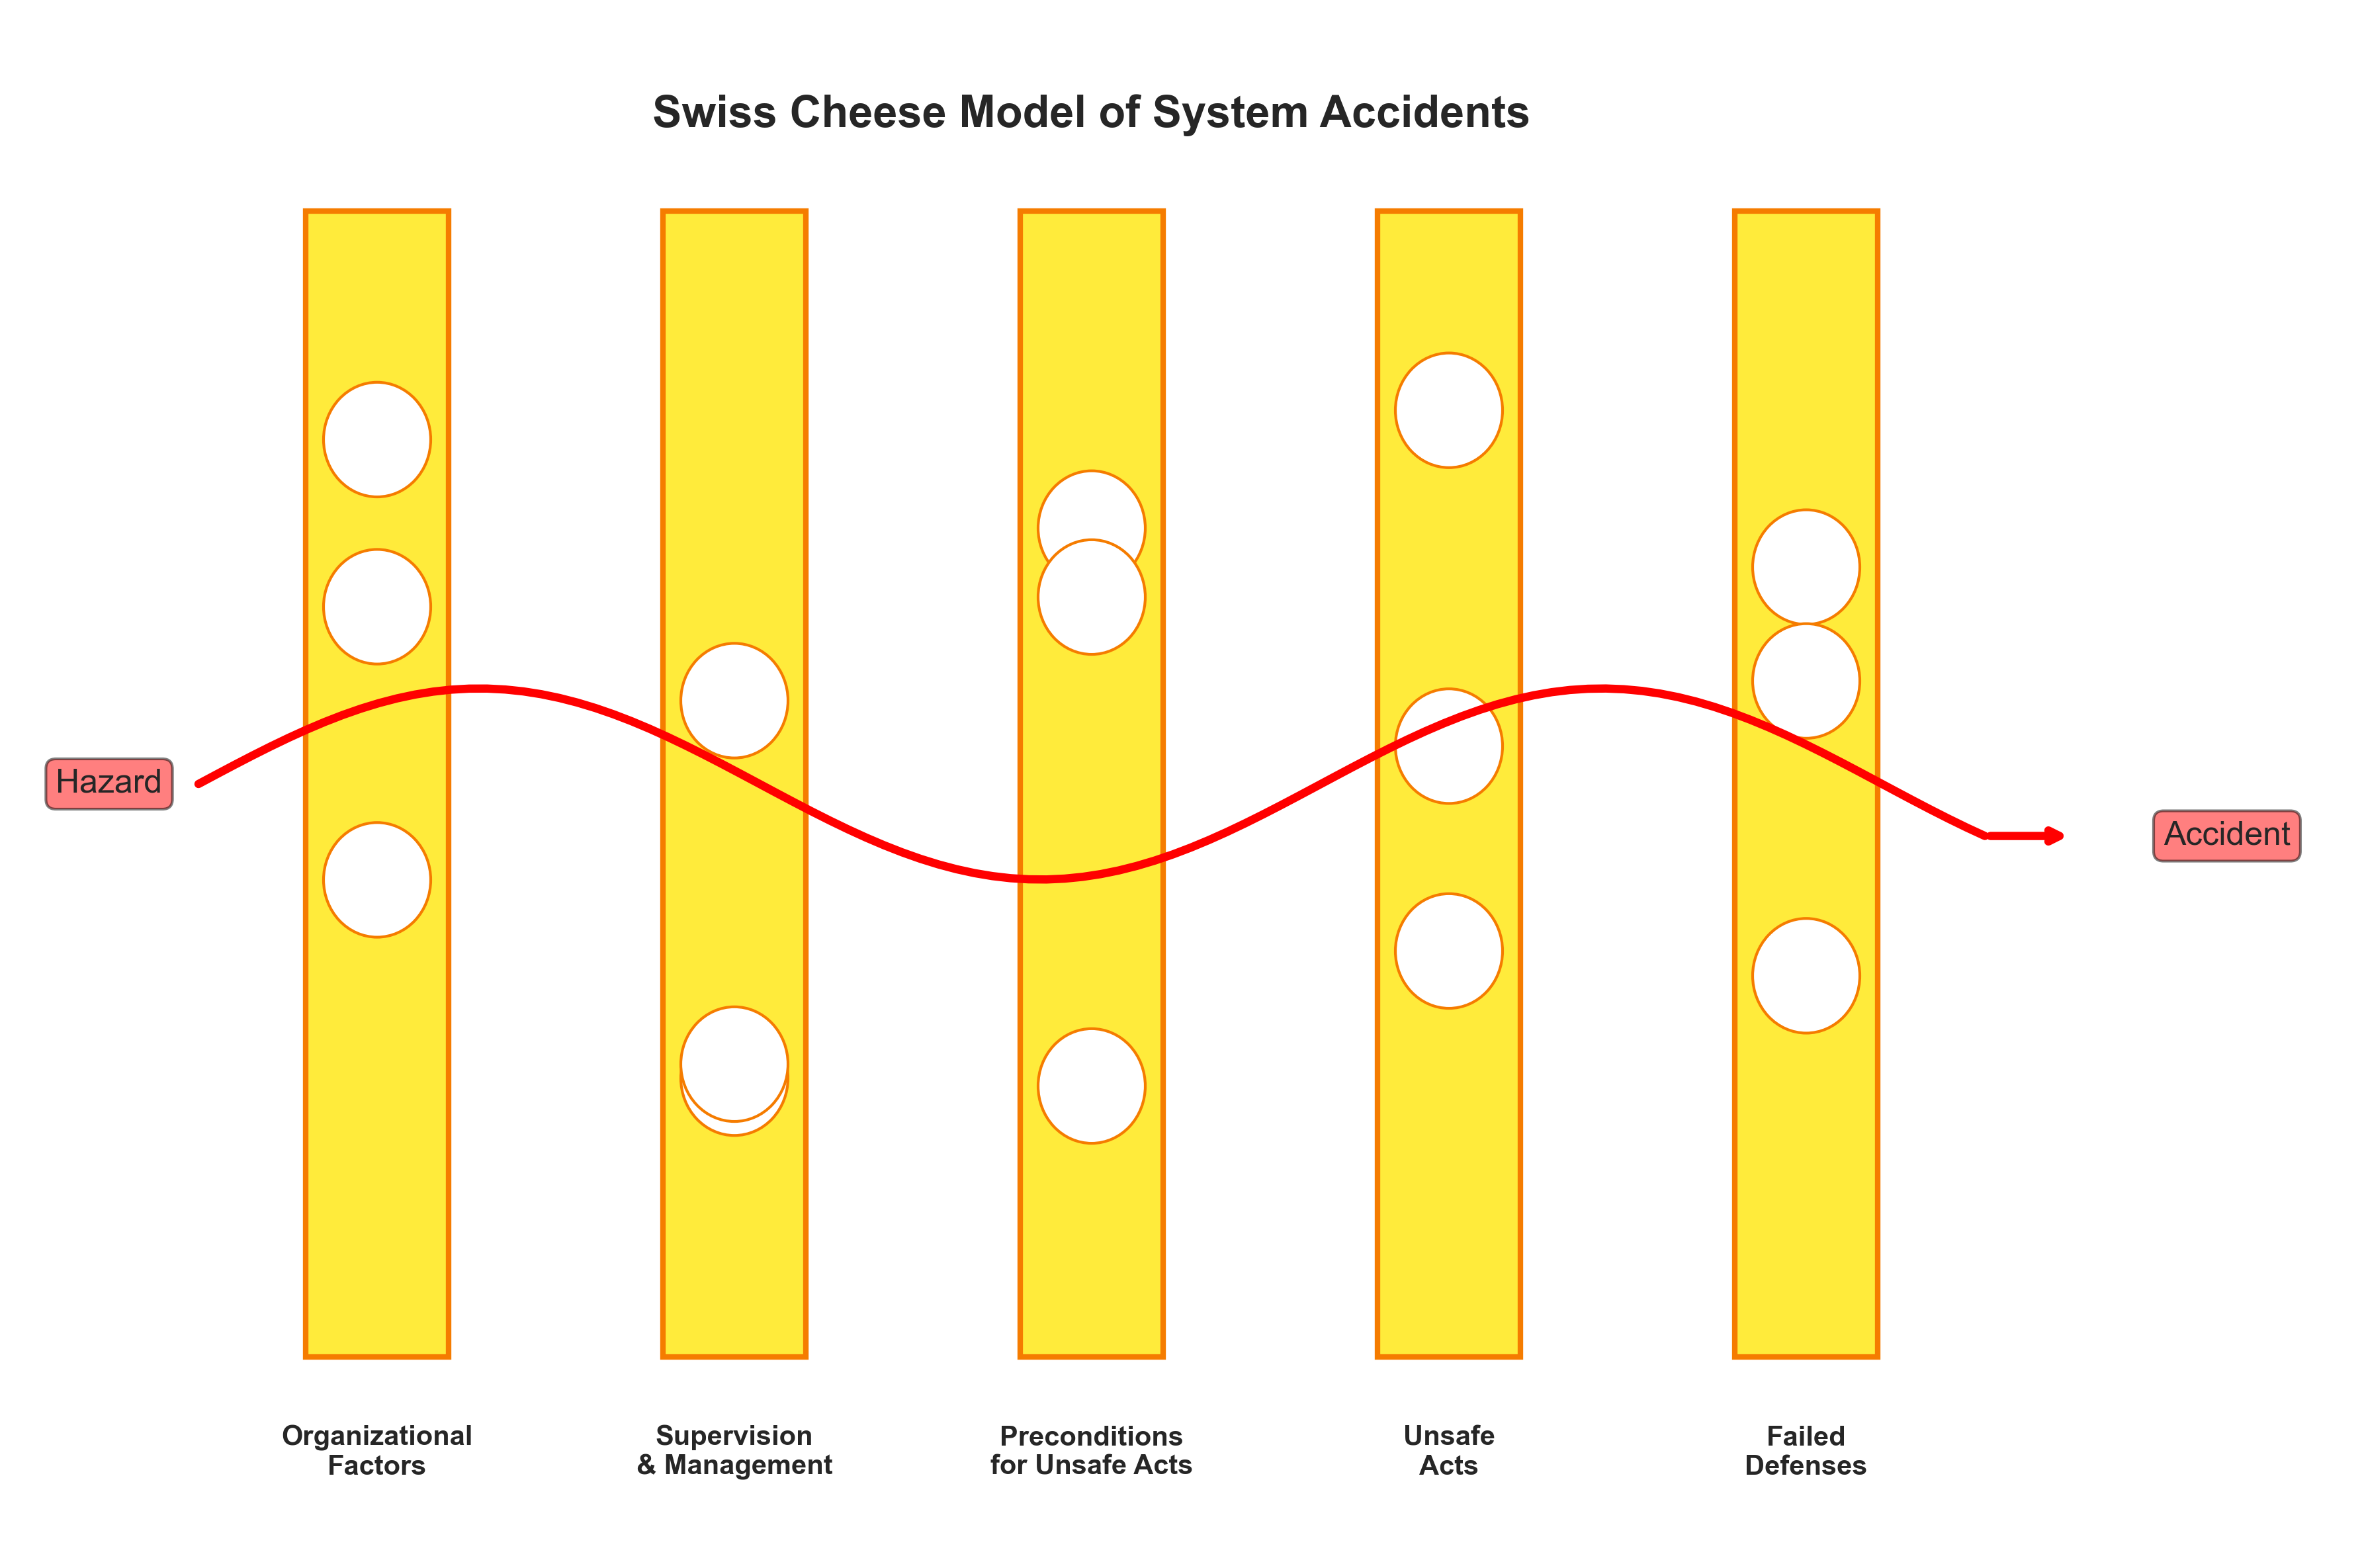
\includegraphics[width=0.85\textwidth]{images/generated/swiss_cheese_model.png}
    \caption{Swiss Cheese Model applied to medication errors, showing how system failures align to cause accidents. Based on Reason's model \citep{ciapponi2021, mulac2020}.}
    \label{fig:swiss_cheese_model}
\end{figure}

\subsection{Clinical Decision Support Systems (CDSS)}

Clinical Decision Support Systems (CDSS) \cite{moss2015, belle2013} and ePrescribing systems have been widely implemented to minimize medication errors \cite{belle2013biomedical, hawley2019}. However, the lack of integration between these modules remains a significant problem. Modern CDSS incorporate features such as real-time interaction checks, guideline-based alerts, and machine learning for personalization \cite{bates2021, zhao2021}.

\subsection{Artificial Intelligence in Healthcare}

The application of Natural Language Processing (NLP) \cite{rozenblum2020} is particularly relevant for extracting drug-drug interaction (DDI) information from unstructured biomedical texts \cite{javaid2022medical}. Systems like the one proposed by Machado \textit{et al.} (2023) use NLP to automatically extract DDI information from scientific literature \cite{machado2023drug}. Tools such as BioBERT have shown promise in this area \cite{Russell2023}. However, low interoperability rates and the absence of universal standards still hinder the widespread adoption of these technologies \citep{Chaya2023}. The development of APIs that can seamlessly integrate data from various hospital systems with NLP and AI platforms is a promising area for further exploration \cite{López2021}.

\subsection{Point-of-care Administration: eMAR and Barcode Medication Administration}
\label{sec:emar_bcma}

Electronic Medication Administration Records (eMAR) and Barcode Medication Administration (BCMA) are key enablers of closed-loop medication management. Literature indicates that linking prescription/validation to bedside administration, with barcode verification of patient, drug and dose, reduces transcription errors and strengthens end-to-end traceability \cite{kallio2020, ciapponi2021}. Integrating eMAR/BCMA into hospital workflows typically requires standardized identifiers, reliable device workflows at the point of care, and near real-time synchronization with pharmacy stock and prescription statuses.

\subsection{Process Standardization and Continuous Improvement}
\label{sec:process_standardization}

Beyond pure technology adoption, standardization of processes (protocols, checklists and harmonized workflows) is a central pillar of safer medication systems. Approaches inspired by Lean and Six Sigma in healthcare focus on reducing waste and variability, clarifying handoffs between roles, and instituting structured control points across the medication cycle. In the context of hospital informatics, standardized digital pathways operationalize these practices by embedding decision logic, validations, and mandatory data elements at each step.

\subsection{Other Emerging Technologies}

Other technologies like Blockchain also show promise for enhancing medication traceability, decentralized consent management, and immutable auditing of prescriptions \cite{franzoso2014}.

\subsection{National and Organizational Context (Portugal)}
\label{sec:national_context_portugal}

In Portugal, the National Health System (SNS) and the Shared Services of the Ministry of Health (SPMS) frame interoperability, security and reporting requirements for hospital information systems. Positioning solutions within this national context—aligning with applicable standards, identifiers and governance practices—facilitates sustainable integration and potential reuse across institutions. Briefly documenting these alignments helps clarify external constraints and opportunities for adoption.

\section{Implementation Architectures and Technologies}

Despite significant advances in hospital process automation, several technical challenges must be overcome. Integrating legacy systems with new technologies requires the standardization of programming languages and communication protocols \cite{stanojevic2023conceptualizing}. Technologies such as Java and Node.js are widely used in backend solutions to ensure scalability, resilience, and data security in critical environments \cite{nkenyereye2016}. Furthermore, the complexity of hospital workflows demands automation that transcends mere data exchange. Real-time synchronization between physician prescriptions, pharmacy stock, and nursing administration is crucial to avoid medication errors, particularly in cases of polypharmacy \citep{Tukukino2022, falconer2021pharmacist}.

\subsection{Architectural Patterns}

Microservices architecture offers several advantages for hospital systems, including independent scalability, resilience to failures, and easier integration with legacy systems \cite{shermock2023, vaghasiya2023, newman2021}. This is often implemented alongside established integration patterns. An API Gateway can serve as a single entry point for all client requests \cite{newman2021}, while a Service Mesh can manage inter-service communication. Adopting an event-driven architecture facilitates asynchronous communication \cite{fowler2018}, and patterns like CQRS (Command Query Responsibility Segregation) can help manage data complexity by separating read and write operations.

\subsection{Standards and Interoperability}

Standards are crucial for achieving interoperability. HL7 FHIR (Fast Healthcare Interoperability Resources) represents the evolution of the HL7 standard, offering native RESTful APIs, modular resources, and support for mobile applications, making it a key enabler for modern, integrated healthcare systems.

\section{Gaps and Opportunities}

The literature review reveals several gaps in existing solutions. The most significant is deficient integration, as current systems often fail to provide seamless interoperability among stakeholders, leading to information silos. This is compounded by usability issues, where interfaces are not optimized for clinical workflows. Additionally, the literature is relatively sparse on unified front-end strategies that modernize legacy ecosystems without full replacement and on operational process standardization approaches tied to informatics. This dissertation addresses these gaps with a non-invasive integration architecture, user-centered design, incremental implementation, and explicit consideration of bedside administration (eMAR/BCMA; Section~\ref{sec:emar_bcma}) and process standardization (Section~\ref{sec:process_standardization}). The use of a centralized backend to orchestrate all processes, from prescription to administration, presents a key opportunity to create a single source of truth and bridge these gaps.

\subsection{Related Implementations (to be populated)}
This subsection will summarize closely related case studies once identified (e.g., unified clinical front-ends over legacy HIS, incremental modernization efforts). It will emphasize architectural choices, change management strategies, and reported outcomes to position this dissertation within comparable initiatives.

\begin{table}[H]
    \centering
    \caption{Comparative analysis of hospital medication management systems including legacy and modern solutions.}
    \label{tab:comparison}
    \begin{tabularx}{\textwidth}{@{}l|X|X|X|X@{}}
        \toprule
        \textbf{Feature} & \textbf{AIDA-PCE} & \textbf{Epic} & \textbf{Cerner} & \textbf{Our System} \\
        \midrule
        Architecture & Monolithic & Integrated Suite & Modular & Microservices \\
        User Interface & Desktop Only & Web/Mobile & Web/Mobile & Responsive Web \\
        Real-time Validation & Limited & Yes & Yes & Advanced \\
        Integration & Custom APIs & HL7/FHIR & HL7/FHIR & RESTful/HL7 \\
        Cloud Support & No & Hybrid & Yes & Cloud-Ready \\
        Cost Model & License & Subscription & Subscription & Open Source \\
        Customization & Limited & Moderate & High & Very High \\
        AI/ML Features & None & Basic & Advanced & Planned \\
        \bottomrule
    \end{tabularx}
\end{table}

\section{Conclusion and Positioning}

The review of the state of the art reveals that despite significant technological advances, a critical gap persists in the interoperability and integration of medication management systems. This work is positioned to address this gap directly. It puts forward a validated model for modernizing hospital workflows through a non-invasive integration strategy, demonstrating that it is possible to create a single, cohesive source of truth without completely replacing legacy infrastructure.

The decision to use enterprise-grade technologies like Java and Node.js was a direct response to the need for secure, scalable, and resilient systems capable of operating in a mission-critical hospital environment. By focusing on a robust backend that orchestrates the entire medication lifecycle, this dissertation presents a pragmatic yet powerful solution to enhance patient safety, improve operational efficiency, and bridge the integration gaps that characterize modern healthcare IT. 

\part{Core of the Dissertation}

% Methodology
\chapter{Methodology}
\label{chap:Methodology}

This chapter details the methodological framework that guided this research. It begins by outlining the high-level research paradigm and strategy, then elaborates on the specific design of the study, the development methodology employed, and the methods used for data collection and evaluation. The chapter concludes with a discussion of ethical considerations and the inherent limitations of the study.

\section{Research Paradigm and Strategy}

This research adopts a \textit{pragmatic paradigm}, integrating quantitative and qualitative methods to address the complex, real-world challenges of hospital medication management \cite{venkatesh2003}. The work is fundamentally grounded in \textit{Design Science Research (\gls{dsr})}, an approach that emphasizes the creation and evaluation of an innovative artifact—in this case, an integrated software system—to solve a concrete organizational problem \cite{martin2017}. This paradigm is ideal as it provides a rigorous structure for developing a technologically sound solution while ensuring its practical relevance and utility within the specific context of the \gls{scmvv} hospital.

To operationalize the DSR paradigm, an \textit{Action Research} strategy is employed \cite{greenhalgh2017}. This choice is dictated by the dynamic nature of the clinical environment, which requires an iterative and adaptive approach. Action Research involves continuous cycles of planning, acting, observing, and reflecting, allowing for the incremental improvement of the system based on empirical feedback gathered directly from healthcare professionals. By making practitioners active partners in the research, this strategy fosters a co-creation of knowledge and ensures the final artifact is deeply aligned with user needs and clinical workflows.

\section{Research Design and Execution}

The project is structured to answer core research questions concerning the impact and implementation of integrated clinical systems. Guiding questions include: 1) How can an integrated system reduce medication errors? 2) What are critical success factors for adoption in a hospital setting? 3) How can its impact be evaluated rigorously?

To address these questions, the work follows a series of structured phases aligned with the work plan (Chapter~\ref{chap:WorkPlan}). The initial \textit{Analysis and Planning} phase focuses on requirement elicitation and a deep analysis of the legacy \gls{aida}-PCE system and current clinical workflows. This analysis is informed by stakeholder input (e.g., interviews and observation) and by reviewing existing processes and data extracts where available, producing process maps and an initial architectural blueprint (see Sections~\ref{sec:context_scmvv} and~\ref{sec:as_is_architecture}).

\subsection{Development and Implementation Methodology}

An adapted \textit{agile methodology} is adopted, combining user-centered design and iterative prototyping to enable continuous engagement with clinicians \cite{fowler2018}. Implementation progresses in focused modules: (i) core infrastructure (security, \gls{jwt}-based authentication, data access), (ii) clinical modules (user/treatment registration, pharmaceutical validation), and (iii) integration with legacy components, namely the \gls{aida}-PCE (Oracle) where applicable. When decision support (\gls{cdss}) features are introduced, they are scoped and validated iteratively with domain stakeholders.

Integration activities emphasize careful mapping of data schemas and safe interoperability with existing systems. The approach privileges incremental integration with legacy assets over big-bang replacement, in line with the overall modernization strategy and the as-is constraints documented in Sections~\ref{sec:context_scmvv} and~\ref{sec:current_process_org}.

Quality assurance activities include functional, integration and performance testing, as well as formative usability assessments with representative users. Performance targets and acceptance criteria are aligned with Chapter~\ref{chap:ExpectedResults} and are verified in controlled test environments prior to any pilot.

\subsection{Research Hypotheses}
The evaluation follows explicit hypotheses to guide measurement and interpretation:
\begin{itemize}
    \item H1: An integrated medication-management system reduces medication errors relative to a documented baseline.
    \item H2: End-to-end process cycle times (prescription to administration) are reduced relative to baseline timings.
    \item H3: User acceptance achieves a "Good" or better outcome on SUS, corroborated by qualitative feedback.
    \item H4: Data coherence across systems improves (fewer redundancies/discrepancies in key fields).
\end{itemize}

\subsection{Risk Management Strategy}

A proactive risk management strategy is integral to the methodology. As detailed in the Risk Analysis of the Work Plan (Section~\ref{sec:RiskAnalysis}), key risks include resistance to change, technical incompatibilities with legacy systems, and potential performance degradation. Mitigation strategies include structured change management (training, stakeholder champions), incremental integration with thorough testing in staging environments, and resilience mechanisms for critical functionalities.

\subsection{Change Management and Training Plan}
A structured change management and training plan accompanies implementation, centered on: (i) early involvement of clinical champions, (ii) short, role-tailored training bursts with practical scenarios, (iii) feedback cycles embedded in sprints, and (iv) quick-reference materials integrated in the UI. Placeholders for training artifacts and schedules are provided in Appendix~\ref{app:details_results} and linked from Results when available.

\section{Data Collection and Evaluation}

To evaluate system impact, a mixed-methods approach to data collection is used, gathering both quantitative and qualitative data during the pilot or evaluation period.

\subsection{Quantitative Data Collection}
Quantitative data focuses on objective, measurable indicators of performance and safety. System performance metrics (e.g., response time, uptime) are monitored. Clinical process data (e.g., medication error rates, task completion times) are compared against baseline data from the legacy system where available. Usage metrics (e.g., active users, feature adoption) are tracked to gauge engagement.

\subsection{Qualitative Data Collection}
Qualitative data provides contextual insights into user experience. In-depth, semi-structured interviews with healthcare professionals and managers are used to understand perceived impact on work. Direct observation of clinical workflows before and after system introduction informs how the system integrates into practice and any unintended consequences or workarounds.

\subsection{Evaluation Criteria}
Success criteria are rooted in the Donabedian model for quality of care (structure, process, outcomes). The specific Key Performance Indicators (KPIs) derived from these criteria are detailed in Chapter~\ref{chap:ExpectedResults} (Section~\ref{sec:KPIs}).

For \textit{Patient Safety}, the primary criterion is a statistically supported reduction in medication errors. For \textit{Operational Efficiency}, success is defined by measurable reductions in process cycle times and improvements in interdisciplinary communication. For \textit{User Acceptance}, evaluation relies on the System Usability Scale (SUS) complemented by qualitative feedback and adoption indicators.

\section{Ethical Considerations and Limitations}

\subsection{Ethical Protocol}
Prior to any data collection or pilot, appropriate ethical approval is obtained from the competent Ethics Committee, and all research activities adhere strictly to the General Data Protection Regulation (GDPR) \cite{european2016}. Patient data is anonymized before analysis, informed consent is sought from participating professionals, and technical/procedural safeguards are implemented to protect confidentiality and integrity.

\subsection{Security, Privacy and Compliance Considerations}
Security and privacy safeguards accompany all stages of the project. Controls include role-based access, authentication and authorization, encrypted communications, immutable audit trails for medication-related actions, and least-privilege principles. Compliance follows applicable legal and institutional requirements (e.g., GDPR), and alignment with national guidance (e.g., SNS/SPMS) is pursued where relevant, as summarized in Section~\ref{sec:national_context_portugal}.

\subsection{Limitations of the Study}
The findings must be interpreted in light of methodological and technical limitations. The single-site case study design may limit generalizability to other hospital contexts. A time-bounded evaluation period may not capture long-term effects on organizational culture or patient outcomes. A pre-post comparison without a parallel control group cannot exclude confounding influences. Finally, reliance on legacy data sources (e.g., Oracle-based \gls{aida}) and the evolving adoption of interoperability standards may impose constraints and suggest directions for future work.



% Work Plan
\chapter{Work Plan}
\label{chap:WorkPlan}

The execution of this dissertation followed a structured 12-month plan, commencing in November 2024 and culminating in the submission in October 2025. This chapter outlines the strategic phasing of the project, designed to ensure a logical progression from foundational research to final implementation and evaluation.

The timeline was organized into five distinct but overlapping phases, each with specific objectives and deliverables. This approach facilitated agile adaptation while maintaining a clear focus on the project's long-term goals. The complete project schedule, including granular tasks and their dependencies, is visualized in the Gantt chart presented in Figure~\ref{fig:gantt_chart_detailed}.

\begin{figure}[htbp]
    \centering
    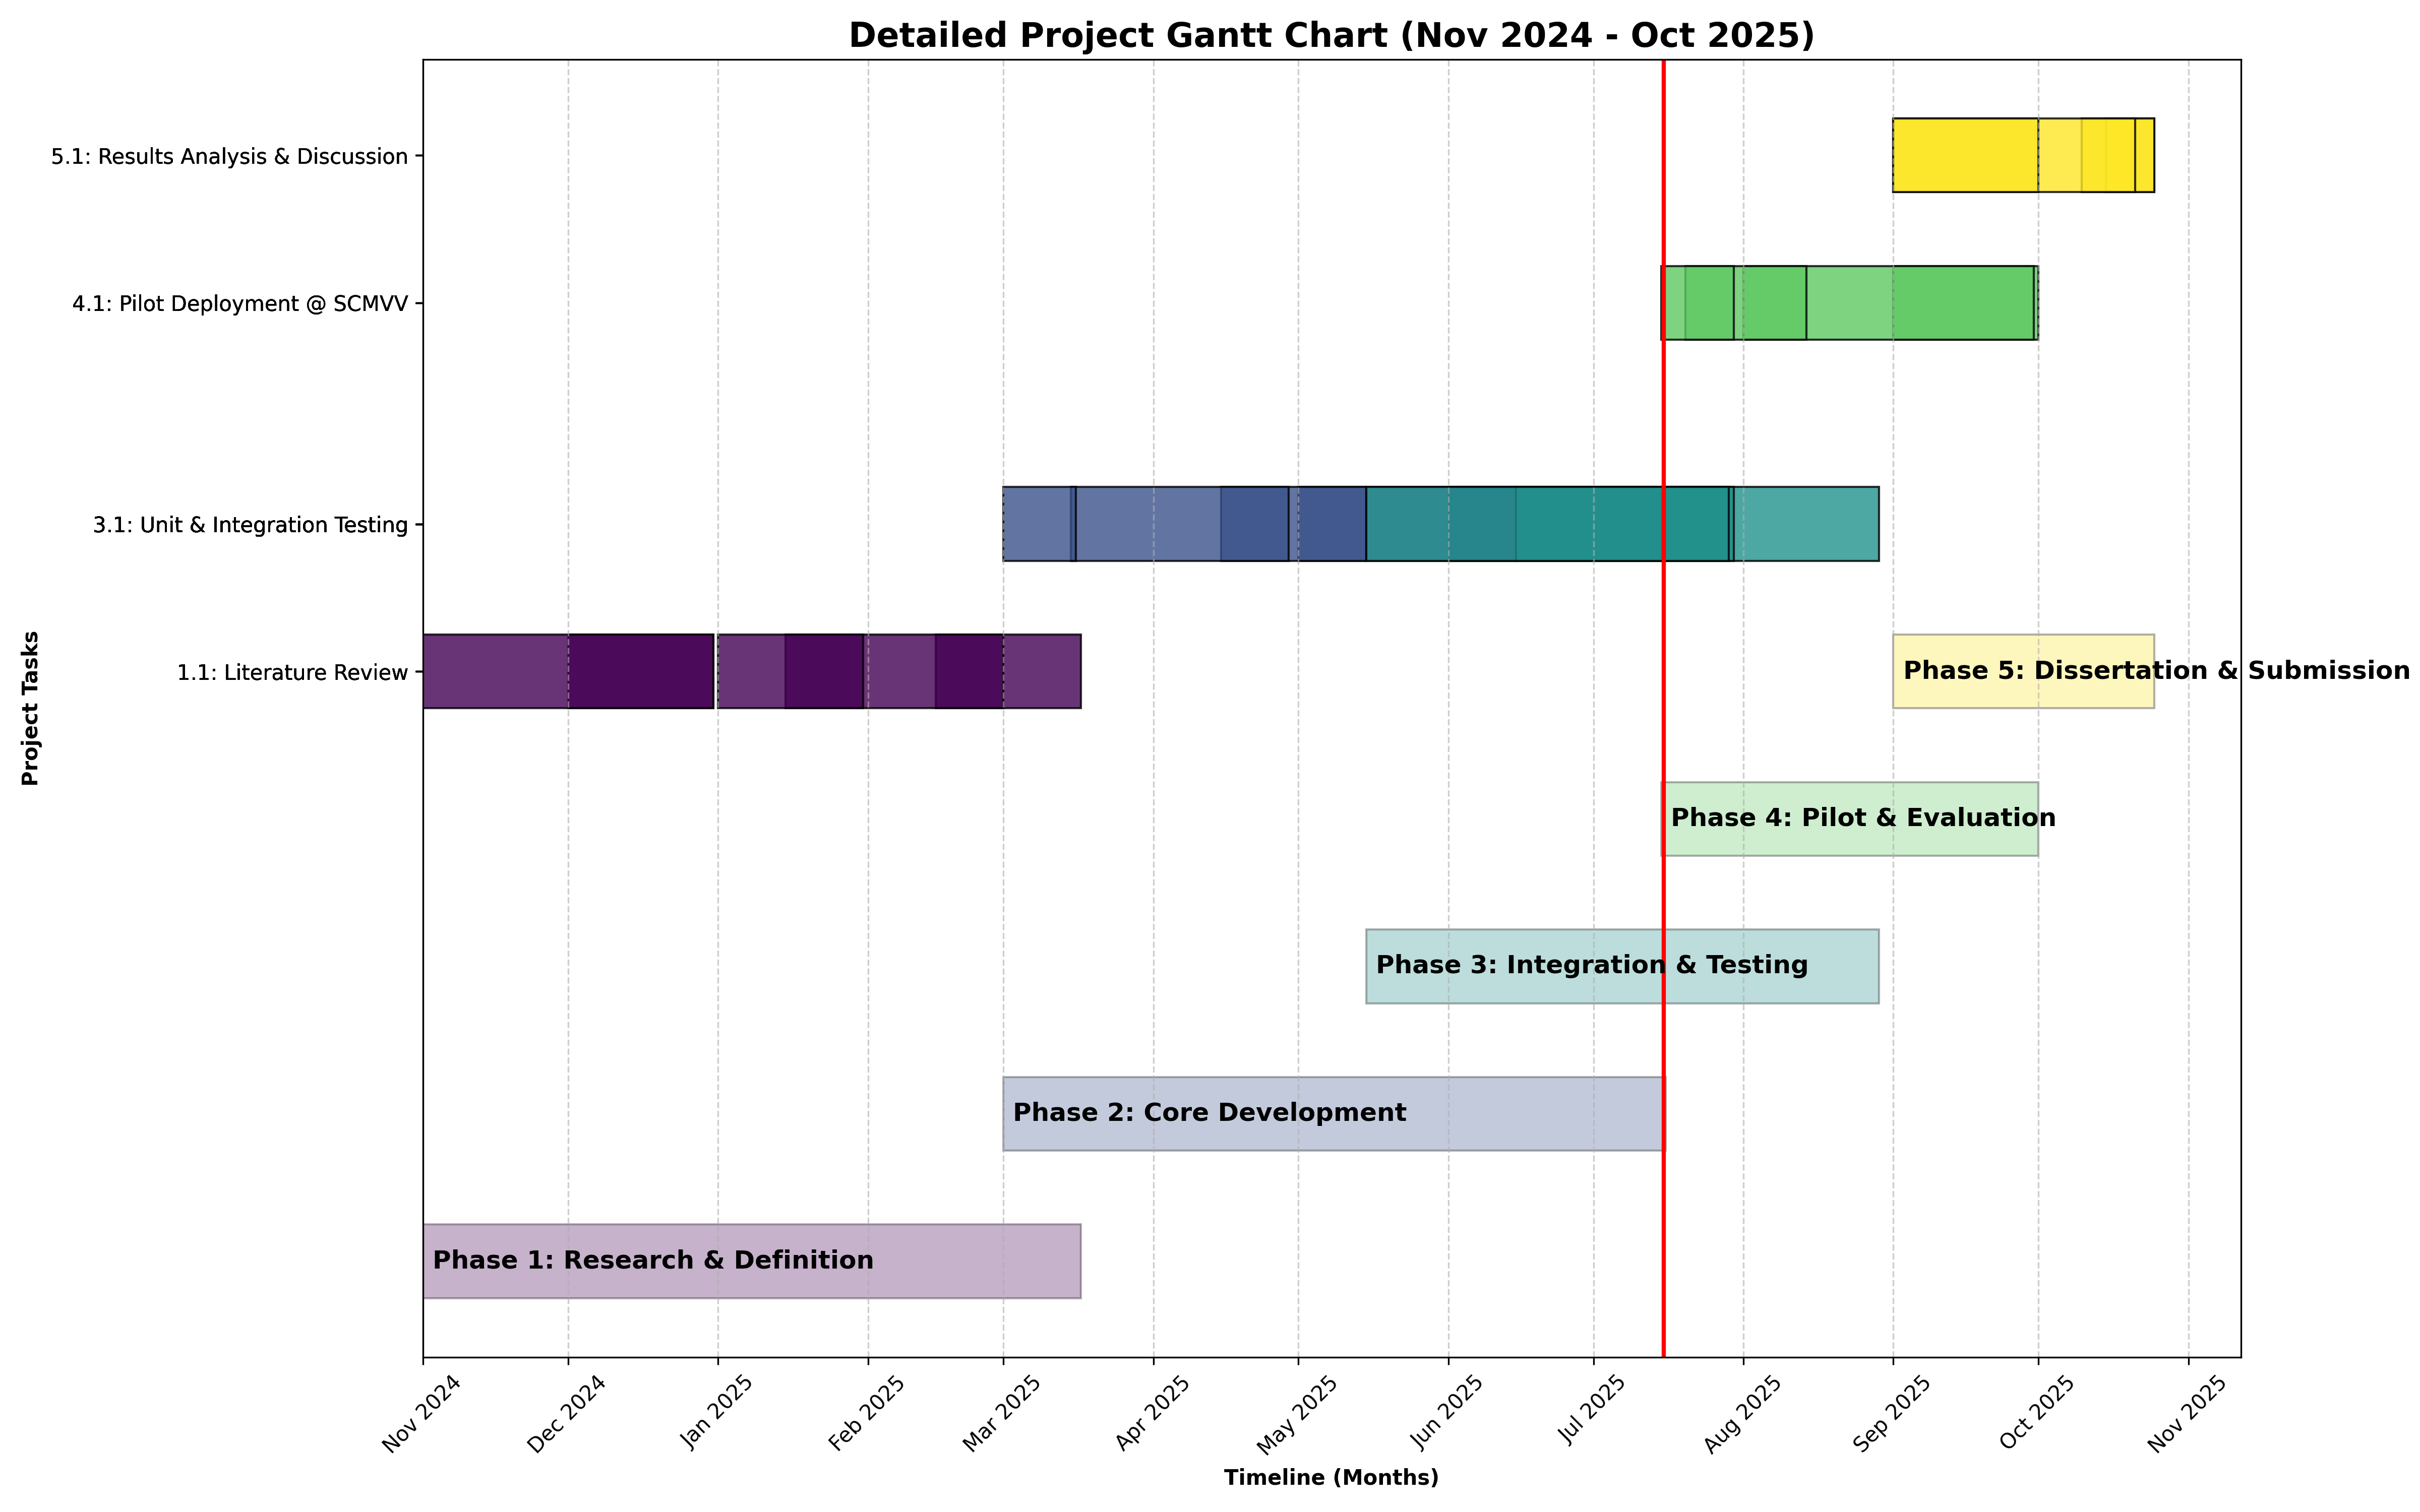
\includegraphics[width=\textwidth]{images/generated/gantt_chart_detailed.png}
    \caption{Detailed Gantt chart illustrating the 12-month project timeline, key phases, and task dependencies from November 2024 to October 2025.}
    \label{fig:gantt_chart_detailed}
\end{figure}

The initial phase, \textit{Research and Definition}, focused on establishing a solid theoretical and empirical foundation through an exhaustive literature review and an in-depth analysis of the existing clinical workflows at SCMVV. This was followed by the \textit{Core Development} phase, where the system's foundational components, including the database, security modules, and core backend logic, were implemented.

Subsequently, the \textit{Integration and Testing} phase ensured that the newly developed modules operated cohesively and could be reliably connected to existing external and legacy systems. The fourth phase, \textit{Pilot and Evaluation}, marked the transition from a development environment to a live clinical setting, where the system was deployed and rigorously evaluated based on user feedback and performance data.

The final phase, \textit{Dissertation and Submission}, was dedicated to the analysis of the collected data, the synthesis of the research findings, and the writing of this dissertation, culminating in its final submission and defense. The detailed methodological framework underpinning the execution of this plan is elaborated upon in the following chapter.

\section{Risk Analysis and Mitigation Strategies}
\label{sec:RiskAnalysis}

A proactive approach to risk management is essential for the successful execution of this project. The risk management plan addresses four key domains: technological, project management, user adoption, and data governance.

The primary technological risk involves integration challenges with the hospital's legacy systems, particularly AIDA-PCE. To mitigate this, a dedicated integration layer will be developed, acting as an anti-corruption shield that isolates the new system from the old. A secondary technical risk pertains to system performance under high load, which will be addressed through continuous load testing and query optimization throughout the development cycle.

In project management, scope creep represents a significant threat. This will be managed through a strict change control process and bi-weekly sprint reviews with stakeholders to ensure alignment with core objectives. Potential delays are mitigated by the modular design, allowing for parallel work streams, and by building buffer time into the project schedule.

A critical sociotechnical risk is the potential for resistance to change from clinical staff. The mitigation strategy is centered on the user-centered co-design approach mentioned in the methodology, ensuring continuous user involvement. This is complemented by a comprehensive training program and the empowerment of clinical champions within each department to drive adoption and provide peer support.

Finally, to address data governance and security risks, compliance with GDPR and robust data protection are paramount. All patient data will be encrypted both at rest and in transit. Access controls will be role-based and strictly enforced, and the system will undergo regular security audits and penetration testing to identify and address vulnerabilities proactively. 
% Expected Results and Evaluation Plan
\chapter{Expected Results and Evaluation Plan}
\label{chap:ExpectedResults}

This chapter outlines the anticipated outcomes of the research and the plan to evaluate the developed system. The expected results are presented across several dimensions: the system's technical architecture, performance and quality benchmarks, clinical impact, user acceptance, and financial viability. The evaluation plan details the methodology, metrics, and instruments that are used to assess success in the intended hospital context.

\section{Proposed System Architecture}

The system's design is guided by the principles of modularity, scalability, and maintainability, culminating in a layered microservices architecture. This architectural choice, illustrated in Figure~\ref{fig:architecture}, is considered critical for managing the complexity of the hospital environment and ensuring a clear separation of concerns. This approach facilitates parallel development, independent deployment of services, and resilience compared to monolithic designs \cite{newman2015}. The as-is baseline and organizational context informing the target design are summarized in Sections~\ref{sec:as_is_architecture} and~\ref{sec:current_process_org}.

\begin{figure}[htbp]
    \centering
    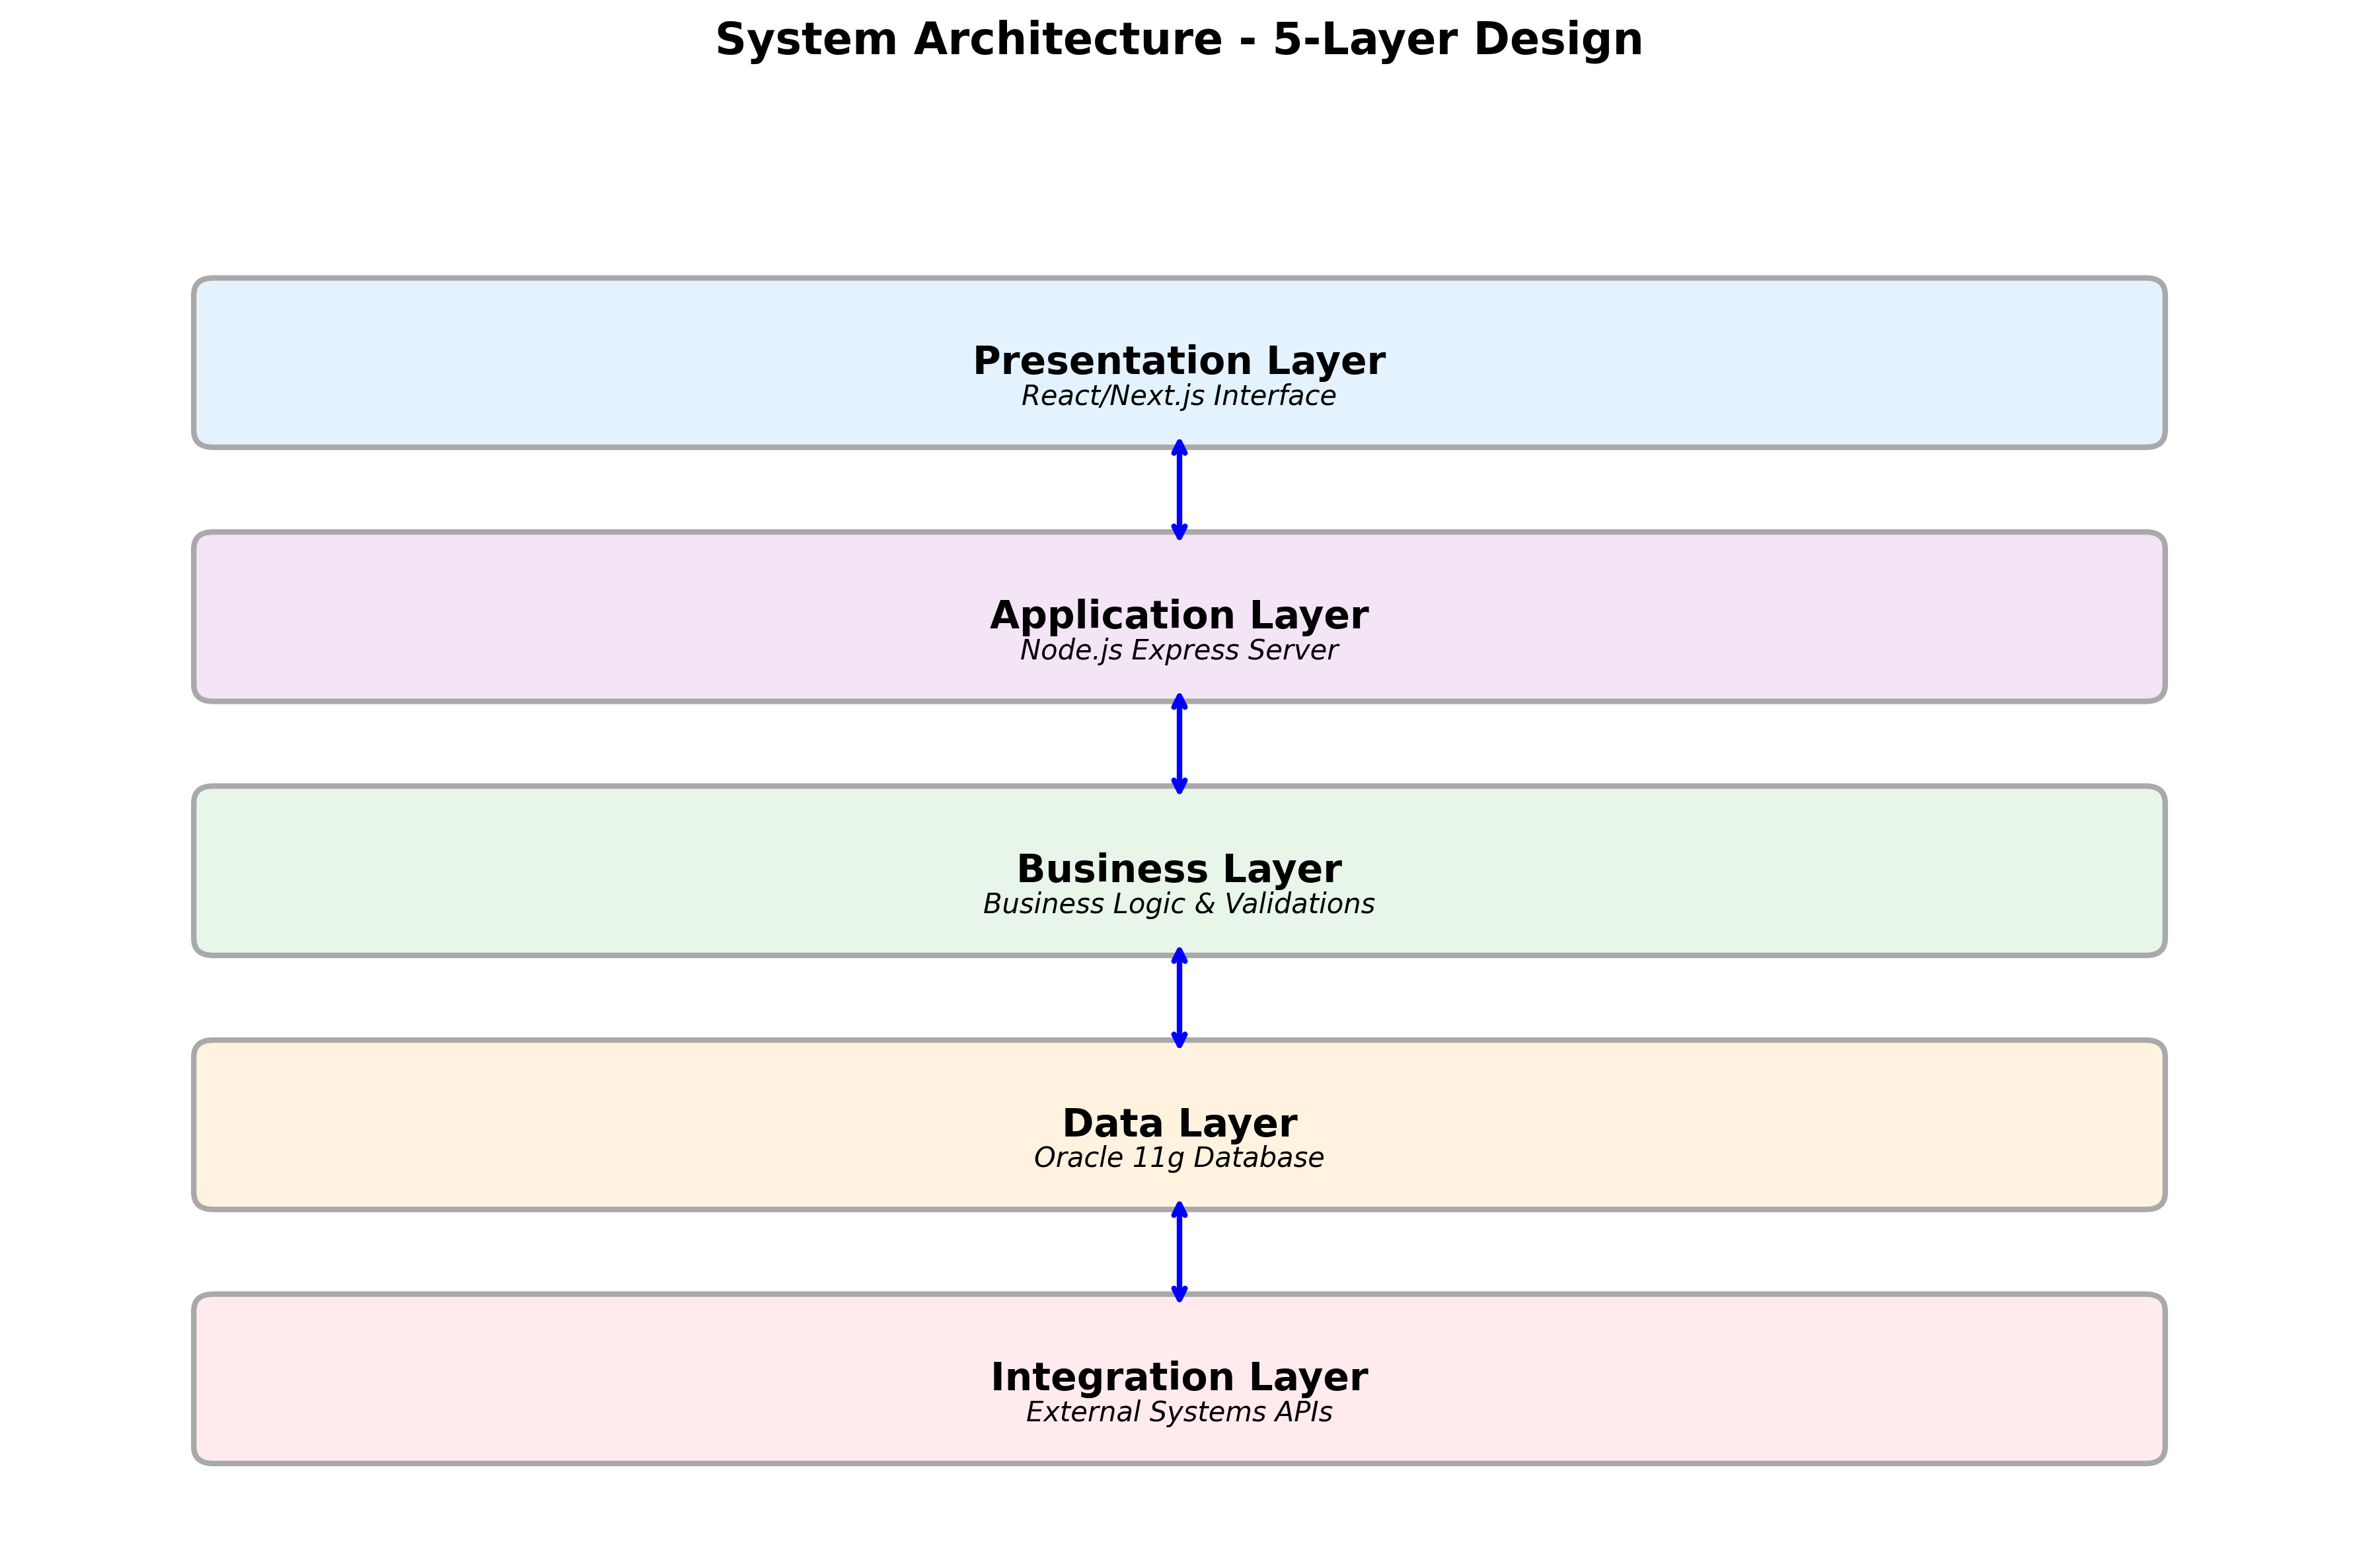
\includegraphics[width=0.95\textwidth]{images/generated/system_architecture.png}
    \caption{Layered architecture of the medication management system, detailing internal components and integrations with external systems.}
    \label{fig:architecture}
\end{figure}

The proposed architecture is organized into five distinct layers. The \textit{Presentation Layer}, built with React and Next.js, provides a responsive and intuitive \gls{ui}. It communicates with the \textit{Application Layer} (Node.js/Express), which orchestrates \glspl{api} requests. Core clinical intelligence resides in the \textit{Business Logic Layer}. Data persistence is handled by the \textit{Data Layer}, using an Oracle database, while the \textit{Integration Layer} provides secure RESTful interfaces for communication with other hospital systems.

Key components include robust authentication (e.g., LDAP-backed \gls{sso}) with granular role-based access control. The e-prescription module includes real-time clinical decision support (\gls{cdss}), aiming to reduce prescribing errors by validating prescriptions against a knowledge base for potential \gls{ddi} and allergies, a strategy supported in the literature \cite{bates2014}. The pharmaceutical validation system is designed to provide a complete and immutable audit trail, enhancing accountability.

\section{Implementation and Artefacts Overview}
This section summarizes implementation artefacts and integration strategies, to be detailed with concrete evidence as available (see Appendix~\ref{app:details_results}).
\begin{itemize}
    \item Artefacto principal (HiSi) (unified frontend/backend): overview of modules for prescription, pharmaceutical validation, administration, and pharmacy stock; technology stack (React/Next.js, Node.js/Express), \gls{jwt}-based authentication, and Oracle connectivity.
    \item Legacy modernization module (e.g., pharmacy PRF): integration with the legacy Oracle schema; description of APIs/routes and UI screens. Evidence to be linked via screenshots/mockups.
    \item Integration strategies considered: (i) submodule embedding vs. (ii) micro-frontend with shared authentication and coordinated routing. Rationale and trade-offs to be documented with references to implementation notes.
    \item Data model overview (legacy integration): placeholder for key tables and relationships involved in stock movements and prescription/validation flows; to be completed from institutional documentation.
\end{itemize}

\subsection*{External Interfaces (to be completed)}
This subsection enumerates external interfaces to be described when specifications are available. Each item includes the intended purpose and a placeholder for protocol/fields.
\begin{itemize}
    \item Billing/administrative reporting: export of events needed for billing and institutional reports. Placeholder: message schema, transport (file/API), validation and reconciliation steps.
    \item Hospital reporting/analytics: periodic extracts for BI dashboards and audit. Placeholder: dataset definitions, aggregation logic, data privacy notes.
    \item National platforms (e.g., \gls{pem}, \gls{sns}/\gls{spms} contexts): scope of possible exchanges (identifiers, prescriptions, confirmations). Placeholder: identifiers used, authentication/authorization model, rate limits.
    \item Security/compliance alignment: logging of access/actions, retention policies, and incident reporting hooks. Placeholder: endpoints/events and audit trail format.
\end{itemize}

\section{Performance and Quality Benchmarks}

Rigorous performance and quality assurance are central to the development methodology. Targeted optimizations aim for low-latency interactions and responsive user experience in clinical settings (e.g., sub-second feedback for critical interactions), using techniques such as efficient querying, caching and judicious precomputation \cite{nielsen2012}.

A primary technical objective is to achieve seamless integration with existing hospital systems, with robust validation and transformation pipelines to minimize synchronization errors. Furthermore, a disciplined testing and refactoring effort increases automated test coverage for critical paths, and the frontend aligns with \gls{wcag} 2.1 Level AA.

\paragraph{Process Standardization and Bedside Administration Alignment}
Expected results include progress toward standardized digital pathways across the medication cycle (protocolized steps, mandatory data elements, and embedded decision checks) and alignment with bedside administration practices (eMAR/BCMA; Section~\ref{sec:emar_bcma}). These outcomes are evidenced through updated flows, UI affordances, and traceability/audit capabilities rather than fixed numerical targets.

\section{Evaluation Plan and Expected Clinical Impact}

Evaluation is planned through a pilot phase at \gls{scmvv} to assess real-world impact. Adoption levels and platform reliability are tracked as key indicators; high availability appropriate for clinical use is a design objective and is confirmed during evaluation \cite{nkenyereye2016}. Comparisons reference the baseline synthesized from legacy analyses (Chapter~\ref{chap:Results}, Section "Baseline from Legacy Analyses").

The intended outcome centers on patient safety. As illustrated conceptually in Figure~\ref{fig:error-reduction}, the project targets a substantial reduction in prescribing and validation errors, consistent with effects reported in the literature \cite{radley2013, bates2014}. End-to-end traceability is expected to shorten incident investigations; concrete magnitudes are established from collected evidence during evaluation.

\begin{figure}[htbp]
    \centering
    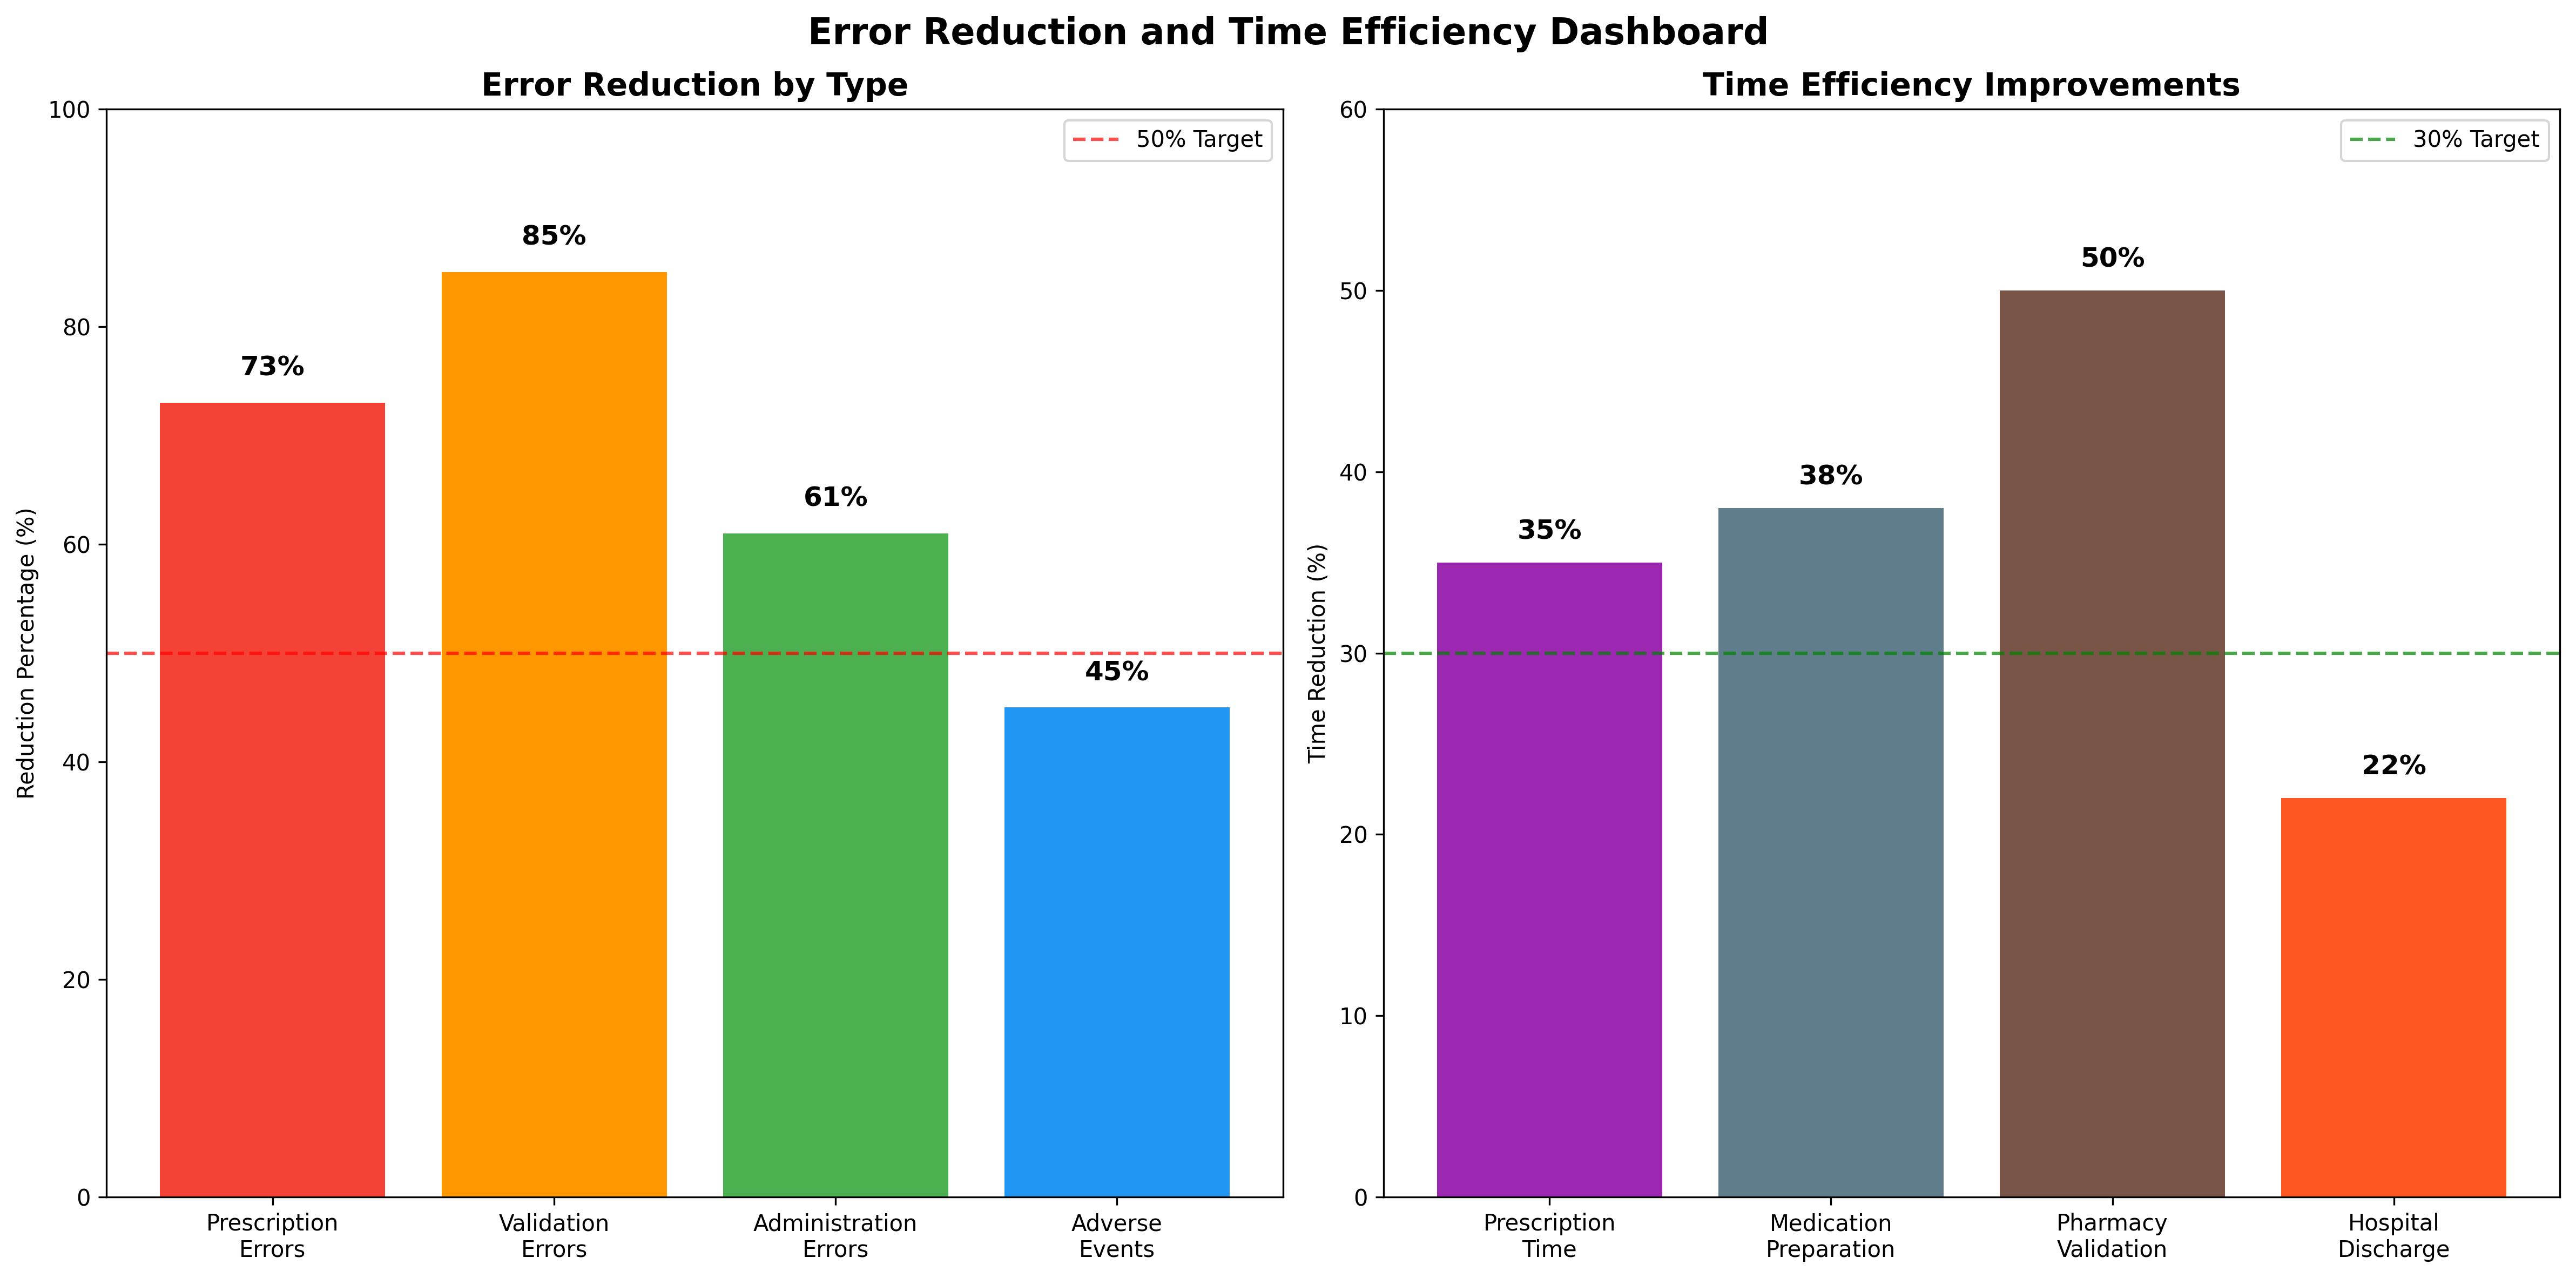
\includegraphics[width=0.95\textwidth]{images/generated/error_reduction_dashboard.png}
    \caption{Dashboard illustrating the reduction in medication errors and improvements in process efficiency following system implementation.}
    \label{fig:error-reduction}
\end{figure}

Operational efficiency gains are also expected. The system streamlines clinical workflows to reduce time to prescribe and validate and to decrease clarification requests, thereby freeing clinical time for patient care \cite{austin2018}. Specific magnitudes are treated as targets to be validated empirically. Alignment with bedside administration practices (eMAR/BCMA; Section~\ref{sec:emar_bcma}) and standardized digital pathways (Section~\ref{sec:process_standardization}) is pursued as part of the objectives.

\section{User Acceptance Evaluation}

High user acceptance is critical for success. User acceptance is evaluated with the System Usability Scale (SUS) and complementary qualitative methods. An acceptable goal is a "Good" or better SUS outcome for the target user groups, to be confirmed by the study \cite{lewis2018}.

Qualitative feedback is collected through semi-structured interviews and focus groups with physicians, pharmacists, and nurses (Figure~\ref{fig:user-satisfaction}). This feedback is analyzed to assess confidence in the system, perceived safety improvements, and workflow clarity. Training time for new users is also monitored with the objective of meaningful reduction compared to the legacy system.

\begin{figure}[htbp]
    \centering
    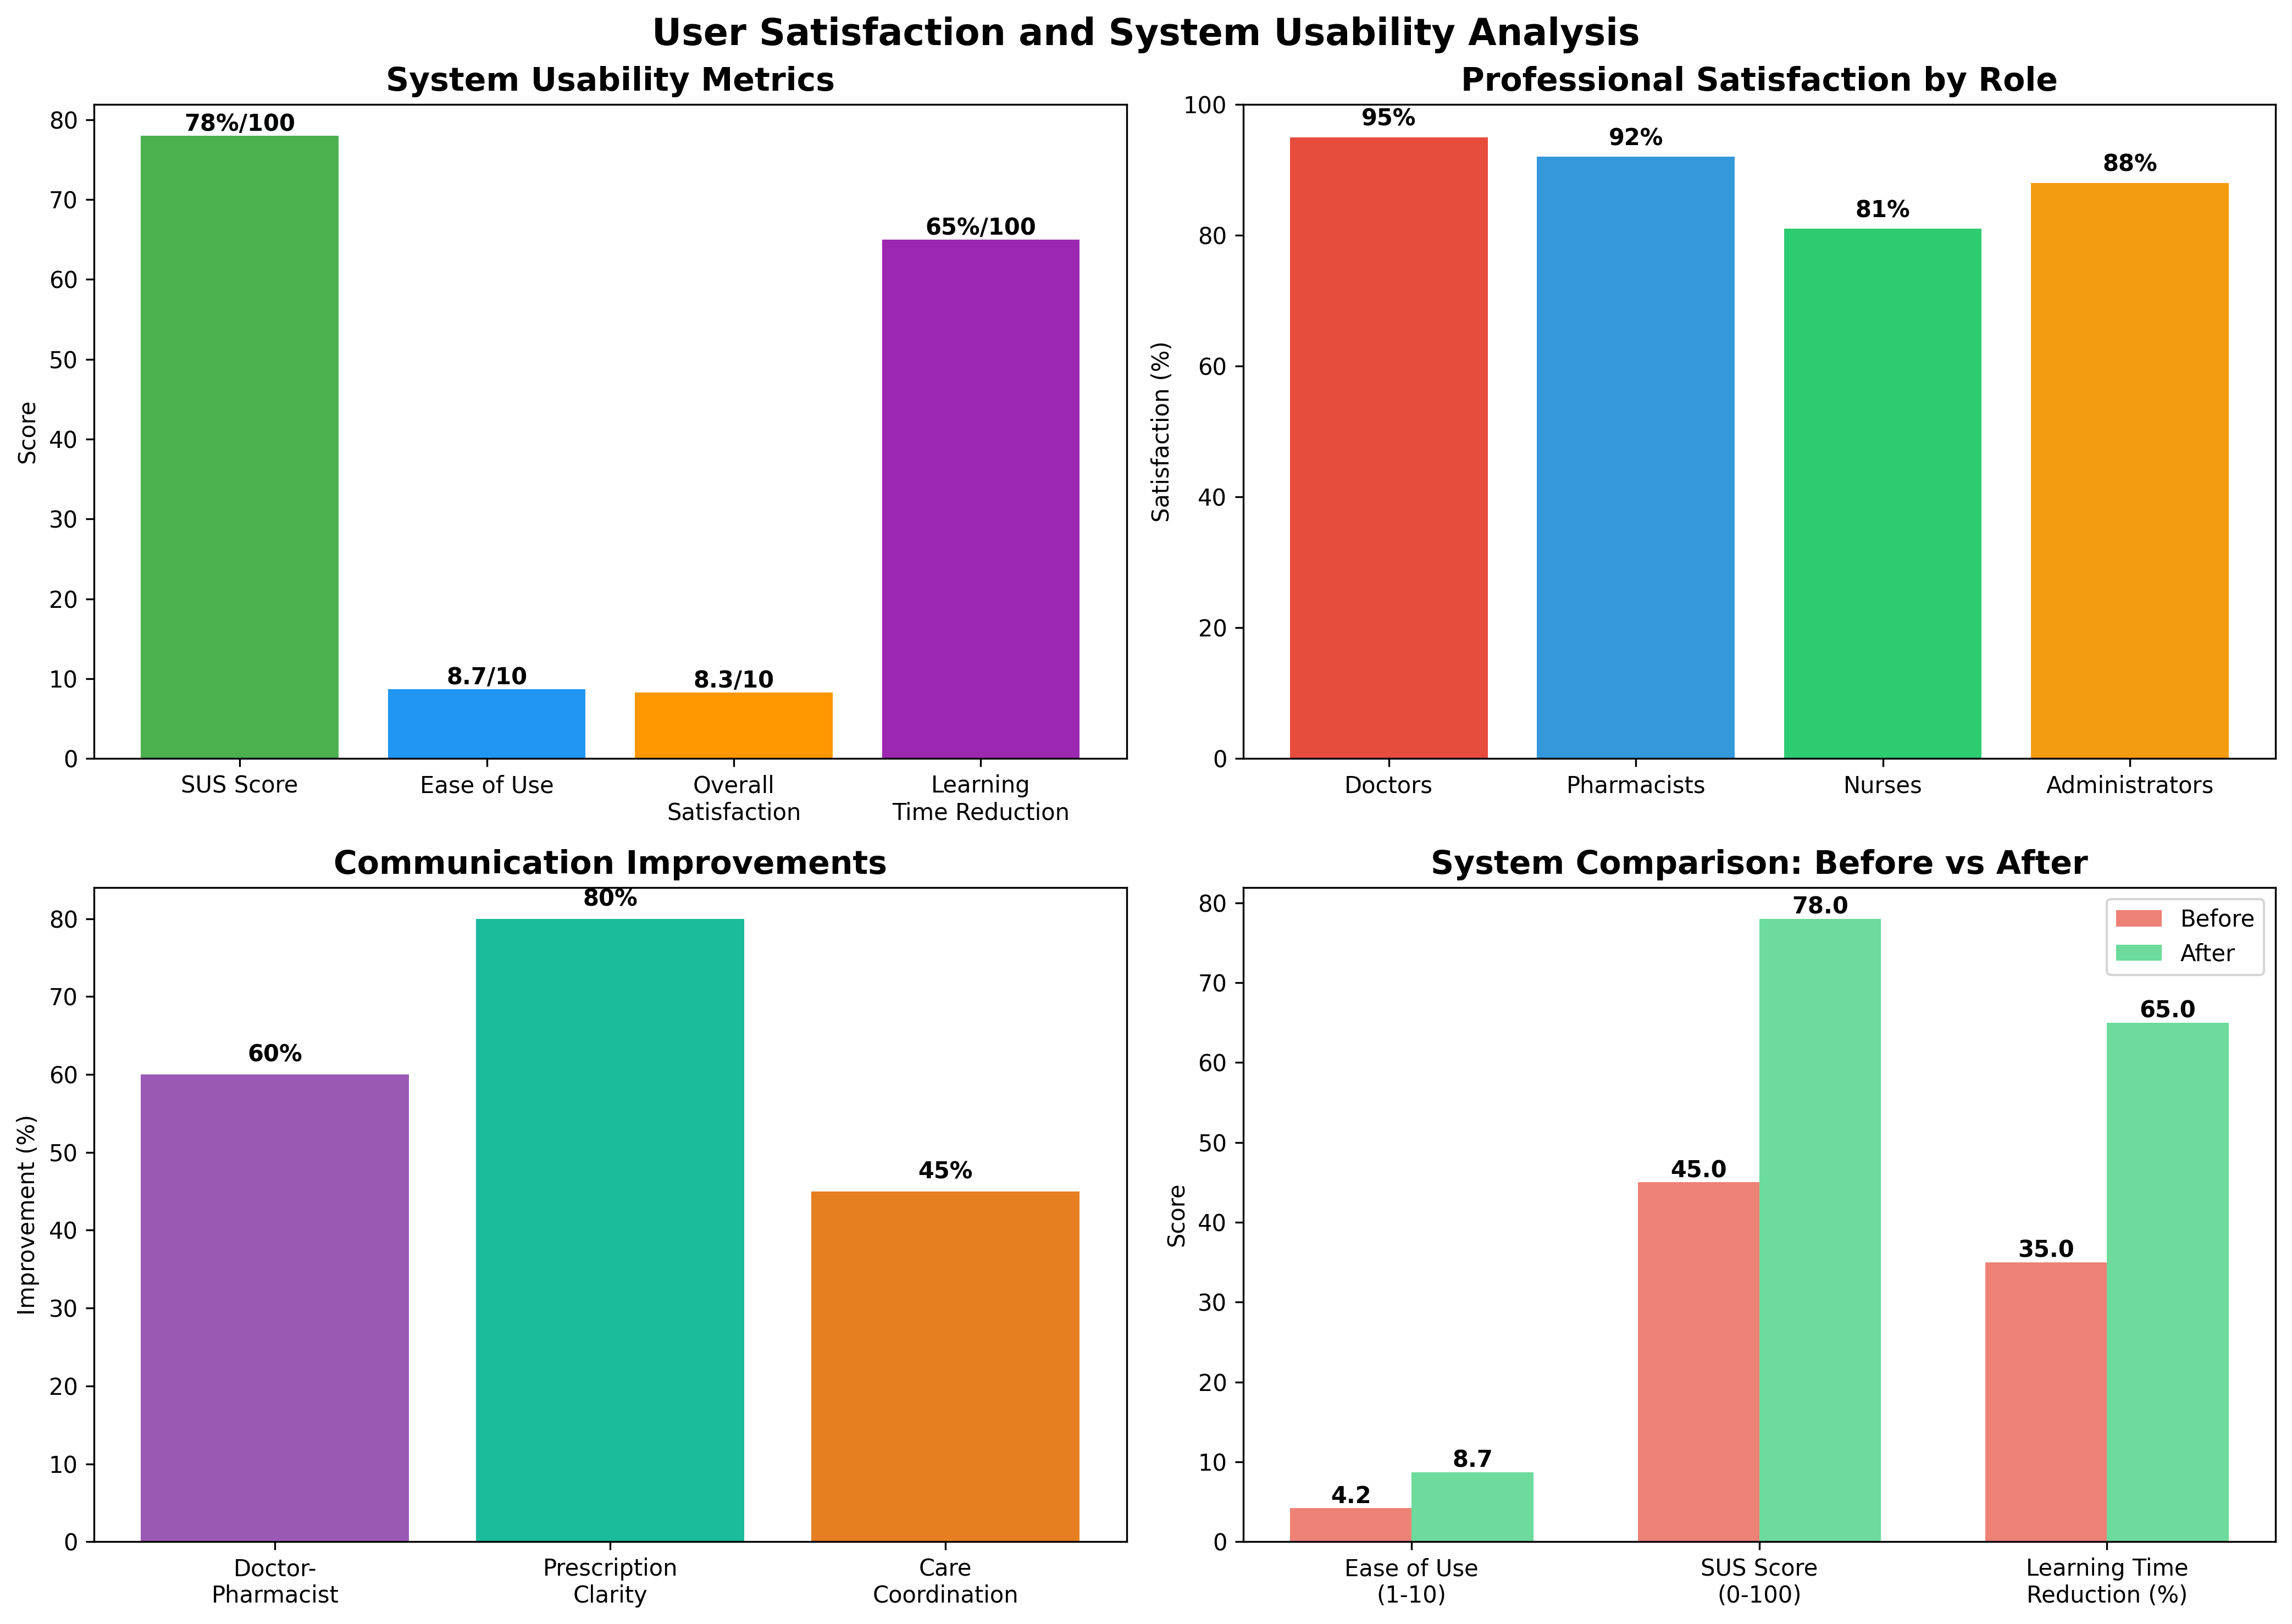
\includegraphics[width=0.95\textwidth]{images/generated/user_satisfaction.png}
    \caption{Comprehensive analysis of user satisfaction, including usability metrics, satisfaction ratings by professional category, and communication improvements.}
    \label{fig:user-satisfaction}
\end{figure}

\section{Expected Financial Impact and Future Viability}

A cost-benefit analysis is conducted as part of the evaluation to determine financial impact. Based on efficiency gains and reduced costs associated with medication errors, Figure~\ref{fig:roi-analysis} summarizes an indicative ROI model; the specific payback period is estimated and validated with study data \cite{adler2021}. Coupled with planned scalability and the strategic roadmap (Figure~\ref{fig:future-roadmap}), this supports long-term viability and potential expansion.

\subsection*{ROI Modelling Note (to be completed)}
This subsection captures the modelling structure to be filled when inputs are available (see Appendix~\ref{app:details_results}).
\begin{itemize}
    \item Inputs (costs): development effort, infrastructure/maintenance, training/change management, opportunity costs vs. licenses avoided.
    \item Inputs (benefits): avoided adverse drug events (unit cost assumptions), efficiency time-savings (per role), reduction of duplicate work, incident investigation time saved.
    \item Assumptions: time horizon, discount rate (if applicable), adoption ramp, conservative vs. optimistic scenarios.
    \item Method: baseline vs. post comparison; sensitivity analysis varying top-3 drivers.
    \item Data sources: institutional documentation (docs/), legacy extracts and analyses (tmp\_ai\_reports/), literature references for unit costs.
\end{itemize}

\begin{figure}[htbp]
    \centering
    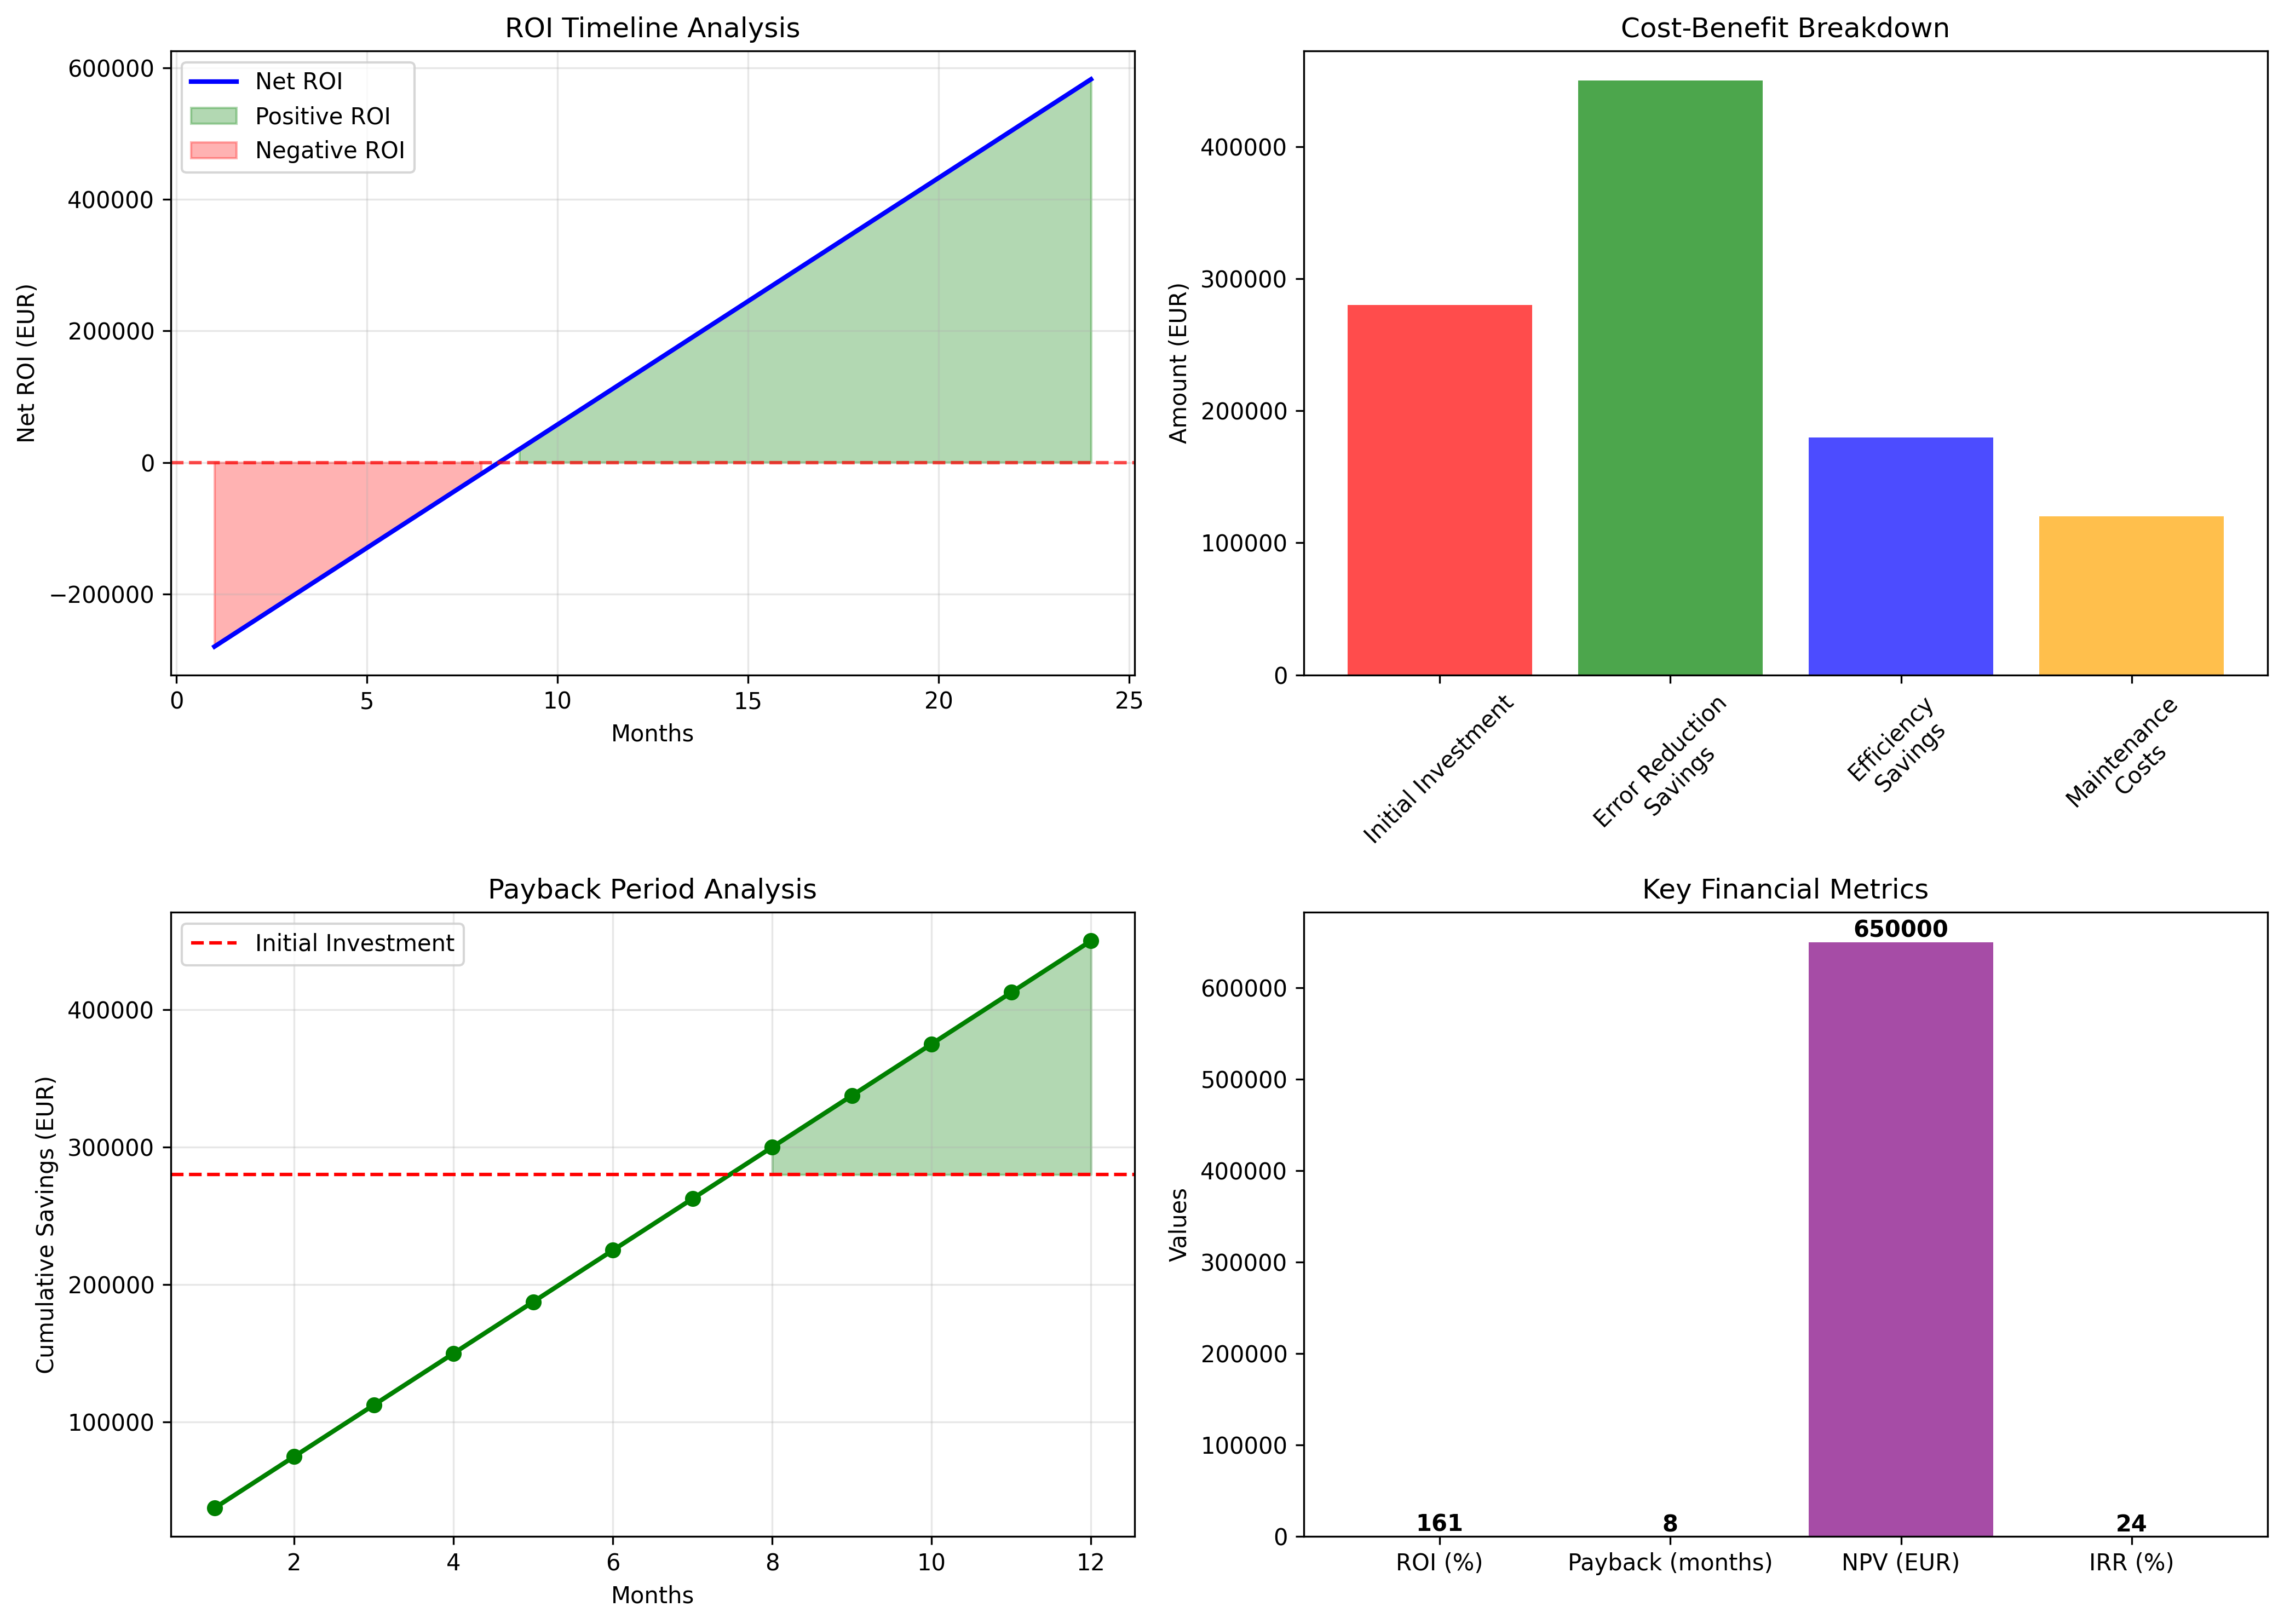
\includegraphics[width=0.95\textwidth]{images/generated/roi_analysis.png}
    \caption{Cost-benefit analysis, including investment breakdown, ROI timeline, and payback period calculation.}
    \label{fig:roi-analysis}
\end{figure}

\begin{figure}[htbp]
    \centering
    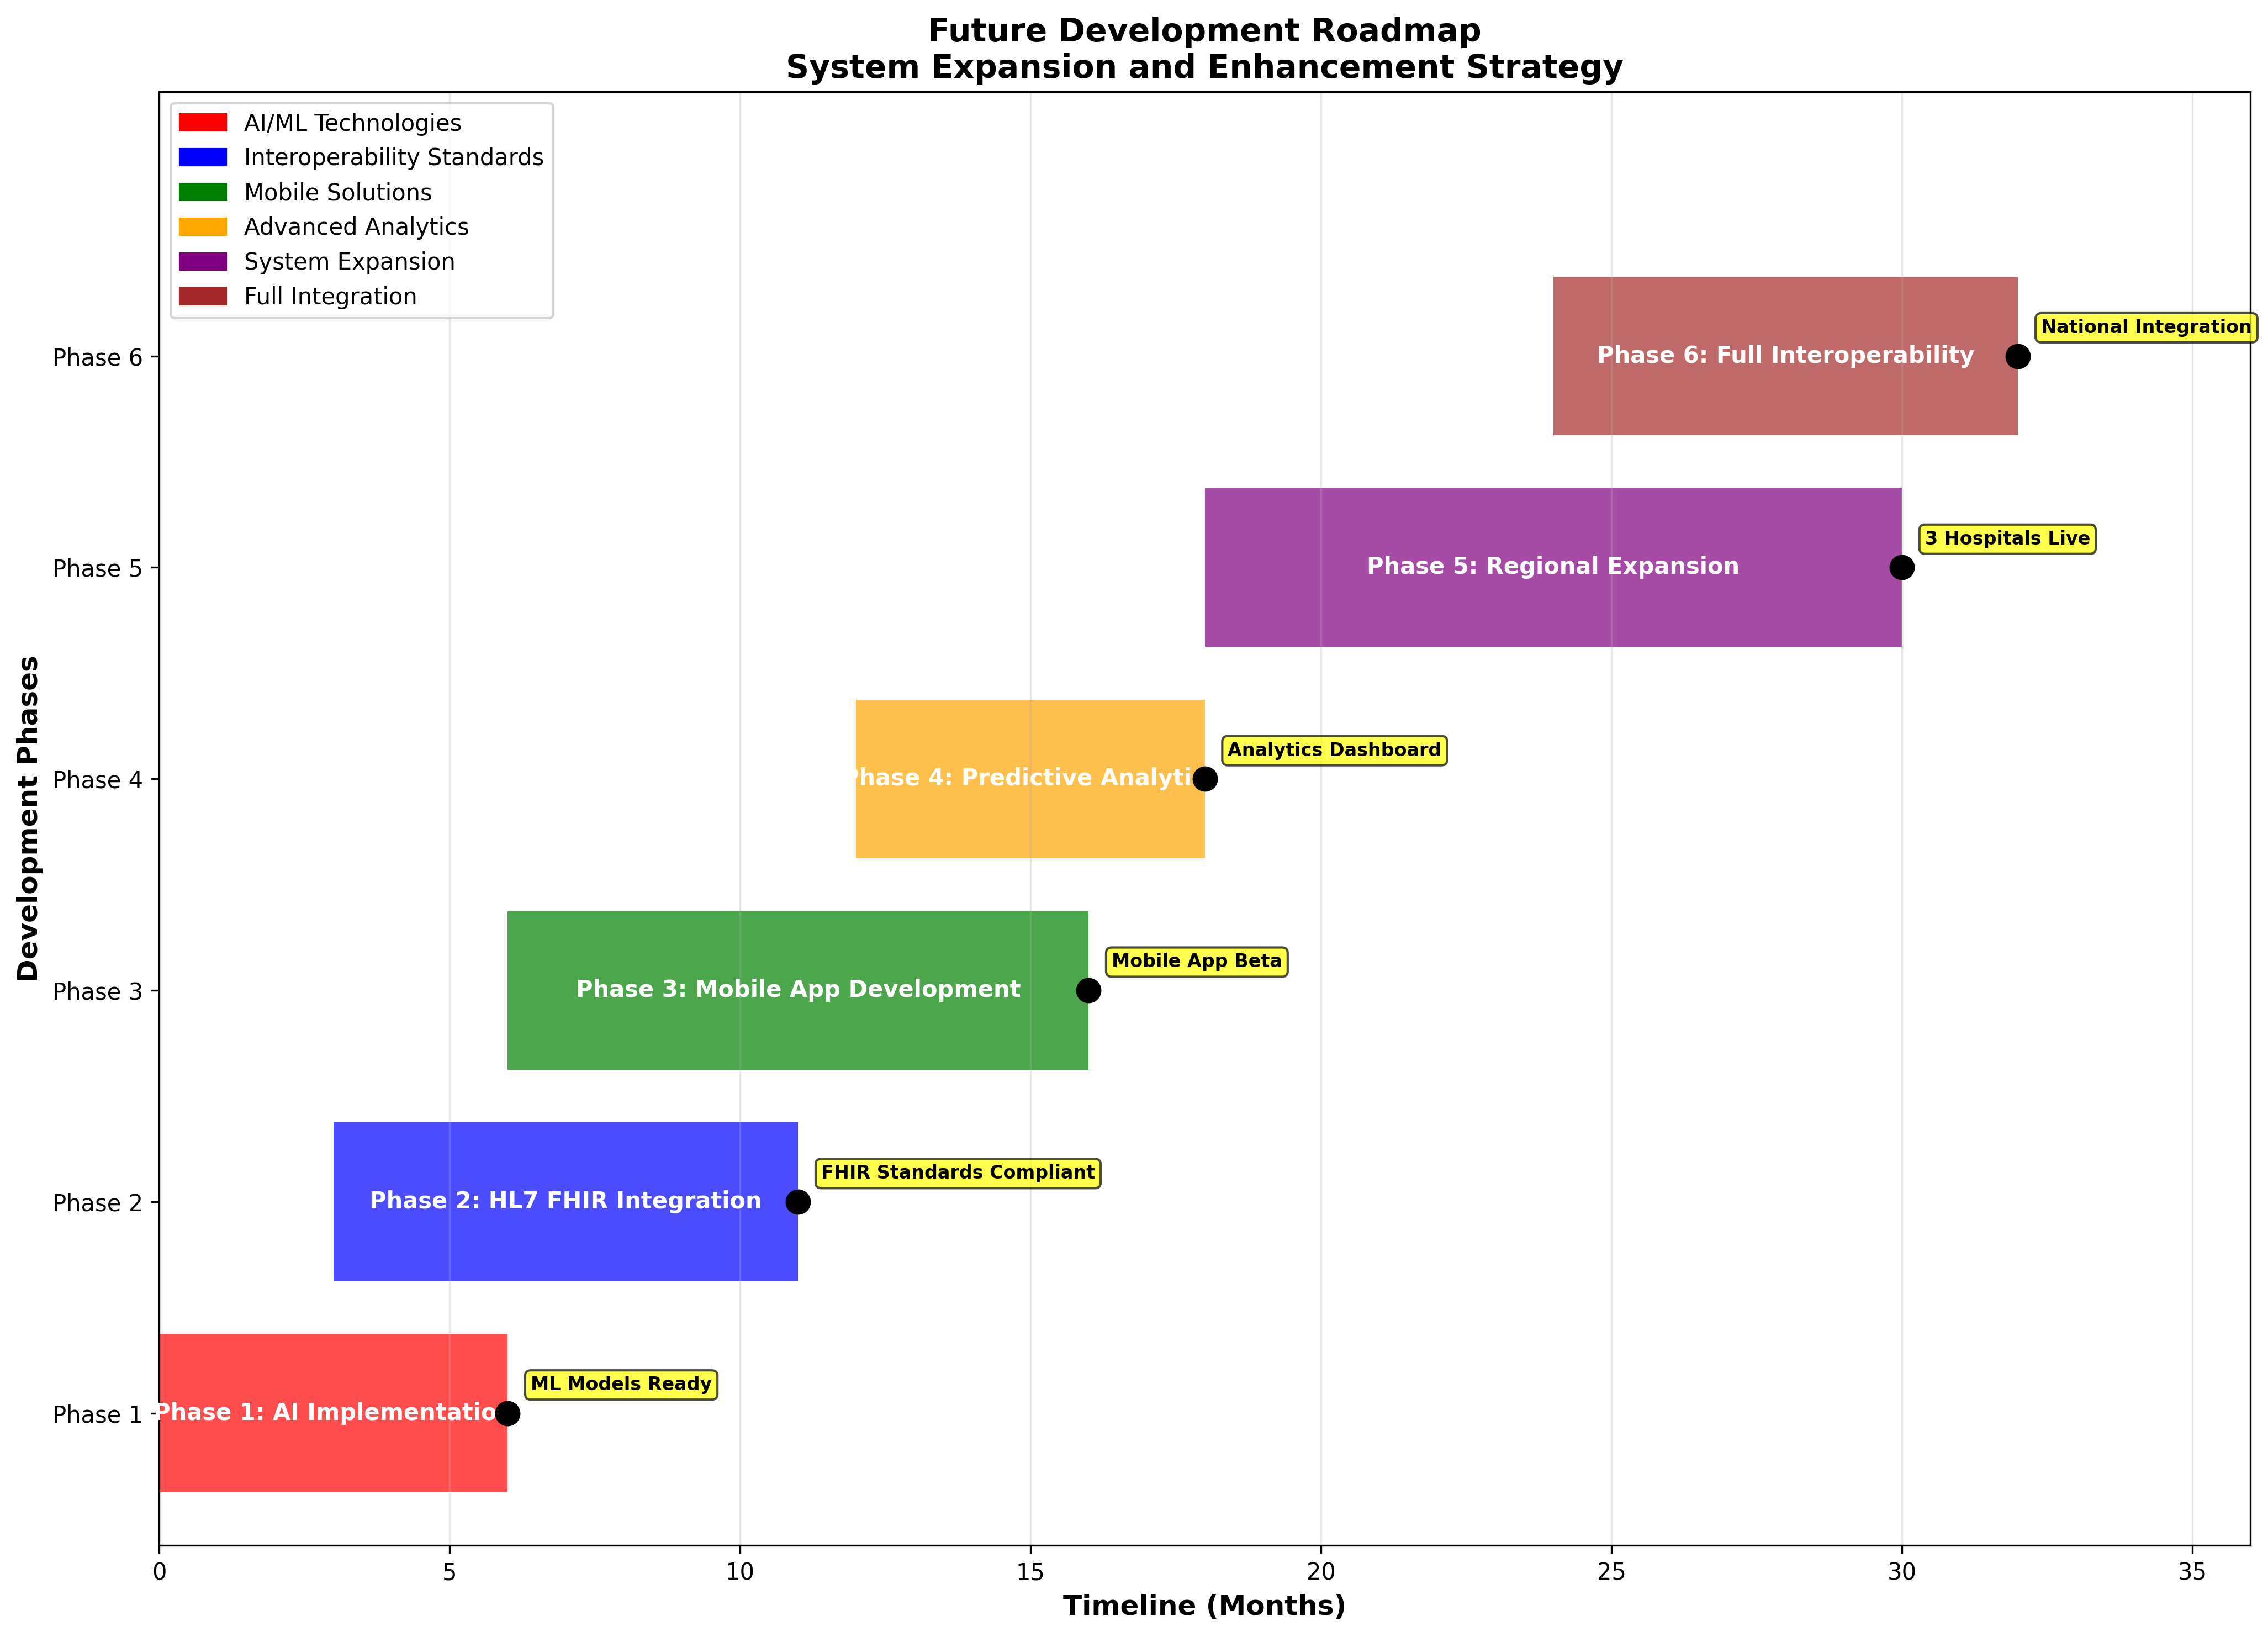
\includegraphics[width=0.95\textwidth]{images/generated/future_roadmap.png}
    \caption{18-month future development roadmap, including AI/ML features, FHIR integration, mobile application development, and regional expansion.}
    \label{fig:future-roadmap}
\end{figure}

\subsection{Key Performance Indicators and Evaluation Scenarios}
\label{sec:KPIs}

To anchor the evaluation in the operational realities of \gls{scmvv}, the pilot focuses on a set of Key Performance Indicators (KPIs), grounded in challenges described by clinical staff and contextualized by fragmentation issues in the Portuguese NHS \cite{goiana2024portuguese, nunes2021articulacao}.

\subsubsection{Patient Safety and Clinical Quality}
The evaluation primarily focuses on reduction in medication errors. This is measured by comparing pre- and post-intervention error rates (e.g., incorrect dosage, wrong medication, missed administrations), using appropriate sample sizes and definitions agreed with stakeholders. Adherence to protocols is assessed by auditing system logs to quantify compliance with integrated clinical decision support rules.

\paragraph{Operational Definitions (to be confirmed)} The following definitions guide measurement without imposing numeric targets: (i) medication error categories (e.g., incorrect dose, wrong drug, missed administration) as defined with stakeholders; (ii) cycle-time start/end anchors (timestamps for order entry, validation decision, dispensing, administration); (iii) adoption proxy measures (active users per role, task completion within system); (iv) reliability indicators (availability windows, error rates of integration pipelines); (v) protocol adherence derived from system logs. Final definitions are documented in the appendix and validated during evaluation.

\subsubsection{Operational Efficiency}
To measure gains in efficiency, the study analyzes time-in-motion for clinical staff, observing the end-to-end process of medication administration before and after system introduction. Additionally, pharmaceutical validation time is measured from prescription entry to final validation, comparing performance against the current multi-system workflow.

\subsubsection{System Integration and Data Integrity}
The success of integration is quantified by measuring reduction in data redundancy and discrepancies. This is achieved through comparative analysis of patient records across relevant systems before and after implementation, identifying inconsistencies in key data fields (e.g., patient identifiers, active medication lists) to demonstrate improvement in data coherence, a known challenge in fragmented health information environments \cite{pinto2016identification}. 
% Results
\chapter{Results}
\label{chap:Results}

This chapter presents practical outcomes to date, focusing on demonstrable artefact capabilities and preliminary evidence. It summarizes system-level deliverables (screens, flows), indicative performance collected in controlled environments, and feedback highlights from stakeholders. These results replace purely prospective statements where measured evidence is available and remain explicitly provisional pending pilot confirmation.

\section{System Demonstration}

\subsection{Prototype Screens and Flows}
Figures in this section illustrate representative screens and end-to-end flows across the unified system (prescribing, pharmaceutical validation, stock updates, and nursing administration). When live screenshots are unavailable in the compilation context, high-fidelity mockups are provided to maintain clarity of the implemented design and interactions.

\paragraph{Role-based legacy context}
In the current legacy setup (AIDA-PCE), functionality is exposed by professional role: medical login for prescription, pharmacist login for validation, and nurse login for administration. The unified artefact aims to streamline these steps while respecting role-based permissions and auditability.

\paragraph{Per-step evidence placeholders}
For each step, insert side-by-side legacy vs. new artifacts when available (or mockups with disclosure):
\begin{itemize}
    \item Prescription: legacy view (AIDA-PCE) vs. unified interface; highlight decision checks and data fields.
    \item Validation: legacy handoff/records vs. in-system validation queue and actions; note audit trail.
    \item Administration: current recording approach (paper/eMAR variability) vs. standardized eMAR flow.
\end{itemize}
Captions must include source (docs/tmp\_ai\_reports) and anonymization note.

% -- Side-by-side: Prescription (legacy vs new)
\begin{figure}[htbp]
    \centering
    \begin{subfigure}[t]{0.44\textwidth}
        \centering
        \imgorplaceholder[width=\linewidth]{images/generated/med_prescricao_utente.png}
        \caption{Prescription (legacy: AIDA-PCE). Source: docs/tmp\_ai\_reports; anonymized.}
        \label{fig:prescription_legacy}
    \end{subfigure}
    \begin{subfigure}[t]{0.44\textwidth}
        \centering
        \imgorplaceholder[width=\linewidth]{images/generated/step_prescription_new_v1.png}
        \caption{Prescription (new unified UI). Source: docs/tmp\_ai\_reports; mockup.}
        \label{fig:prescription_new}
    \end{subfigure}
    \caption{Side-by-side prescription flow: legacy vs. unified interface.}
\end{figure}

% -- Side-by-side: Validation (legacy vs new)
\begin{figure}[htbp]
    \centering
    \begin{subfigure}[t]{0.37\textwidth}
        \centering
        \imgorplaceholder[width=\linewidth]{images/generated/baseline_validation_queue_v1.png}
        \caption{Validation (legacy: AIDA-PCE). Source: docs/tmp\_ai\_reports; anonymized.}
        \label{fig:validation_legacy}
    \end{subfigure}
    \begin{subfigure}[t]{0.37\textwidth}
        \centering
        \imgorplaceholder[width=\linewidth]{images/generated/step_validation_new_v1.png}
        \caption{Validation (new unified UI). Source: docs/tmp\_ai\_reports; mockup.}
        \label{fig:validation_new}
    \end{subfigure}
    \caption{Side-by-side pharmaceutical validation: legacy vs. unified interface.}
\end{figure}

% -- Side-by-side: Administration (legacy vs new)
\begin{figure}[htbp]
    \centering
    \begin{subfigure}[t]{0.37\textwidth}
        \centering
        \imgorplaceholder[width=\linewidth]{images/generated/enf_administracao_utente.png}
        \caption{Administration (legacy: AIDA-PCE e/ou eMAR atual). Source: docs/tmp\_ai\_reports; anonymized.}
        \label{fig:administration_legacy}
    \end{subfigure}
    \begin{subfigure}[t]{0.37\textwidth}
        \centering
        \imgorplaceholder[width=\linewidth]{images/generated/step_administration_new_v1.png}
        \caption{Administration (new eMAR flow). Source: docs/tmp\_ai\_reports; mockup.}
        \label{fig:administration_new}
    \end{subfigure}
    \caption{Side-by-side nursing administration: legacy vs. unified eMAR.}
\end{figure}

% -- Side-by-side: Stock movements (legacy vs new)
\begin{figure}[htbp]
    \centering
    \begin{subfigure}[t]{0.38\textwidth}
        \centering
        \imgorplaceholder[width=\linewidth]{images/generated/baseline_lista_zero_v1.png}
        \caption{Stock movements (legacy: AIDA-PCE/PRF). Source: docs/tmp\_ai\_reports; anonymized.}
        \label{fig:stock_legacy}
    \end{subfigure}
    \begin{subfigure}[t]{0.38\textwidth}
        \centering
        \imgorplaceholder[width=\linewidth]{images/generated/step_stock_new_v1.png}
        \caption{Stock movements (new PRF module). Source: docs/tmp\_ai\_reports; mockup.}
        \label{fig:stock_new}
    \end{subfigure}
    \caption{Side-by-side stock management: legacy vs. unified module.}
\end{figure}

\begin{figure}[htbp]
    \centering
    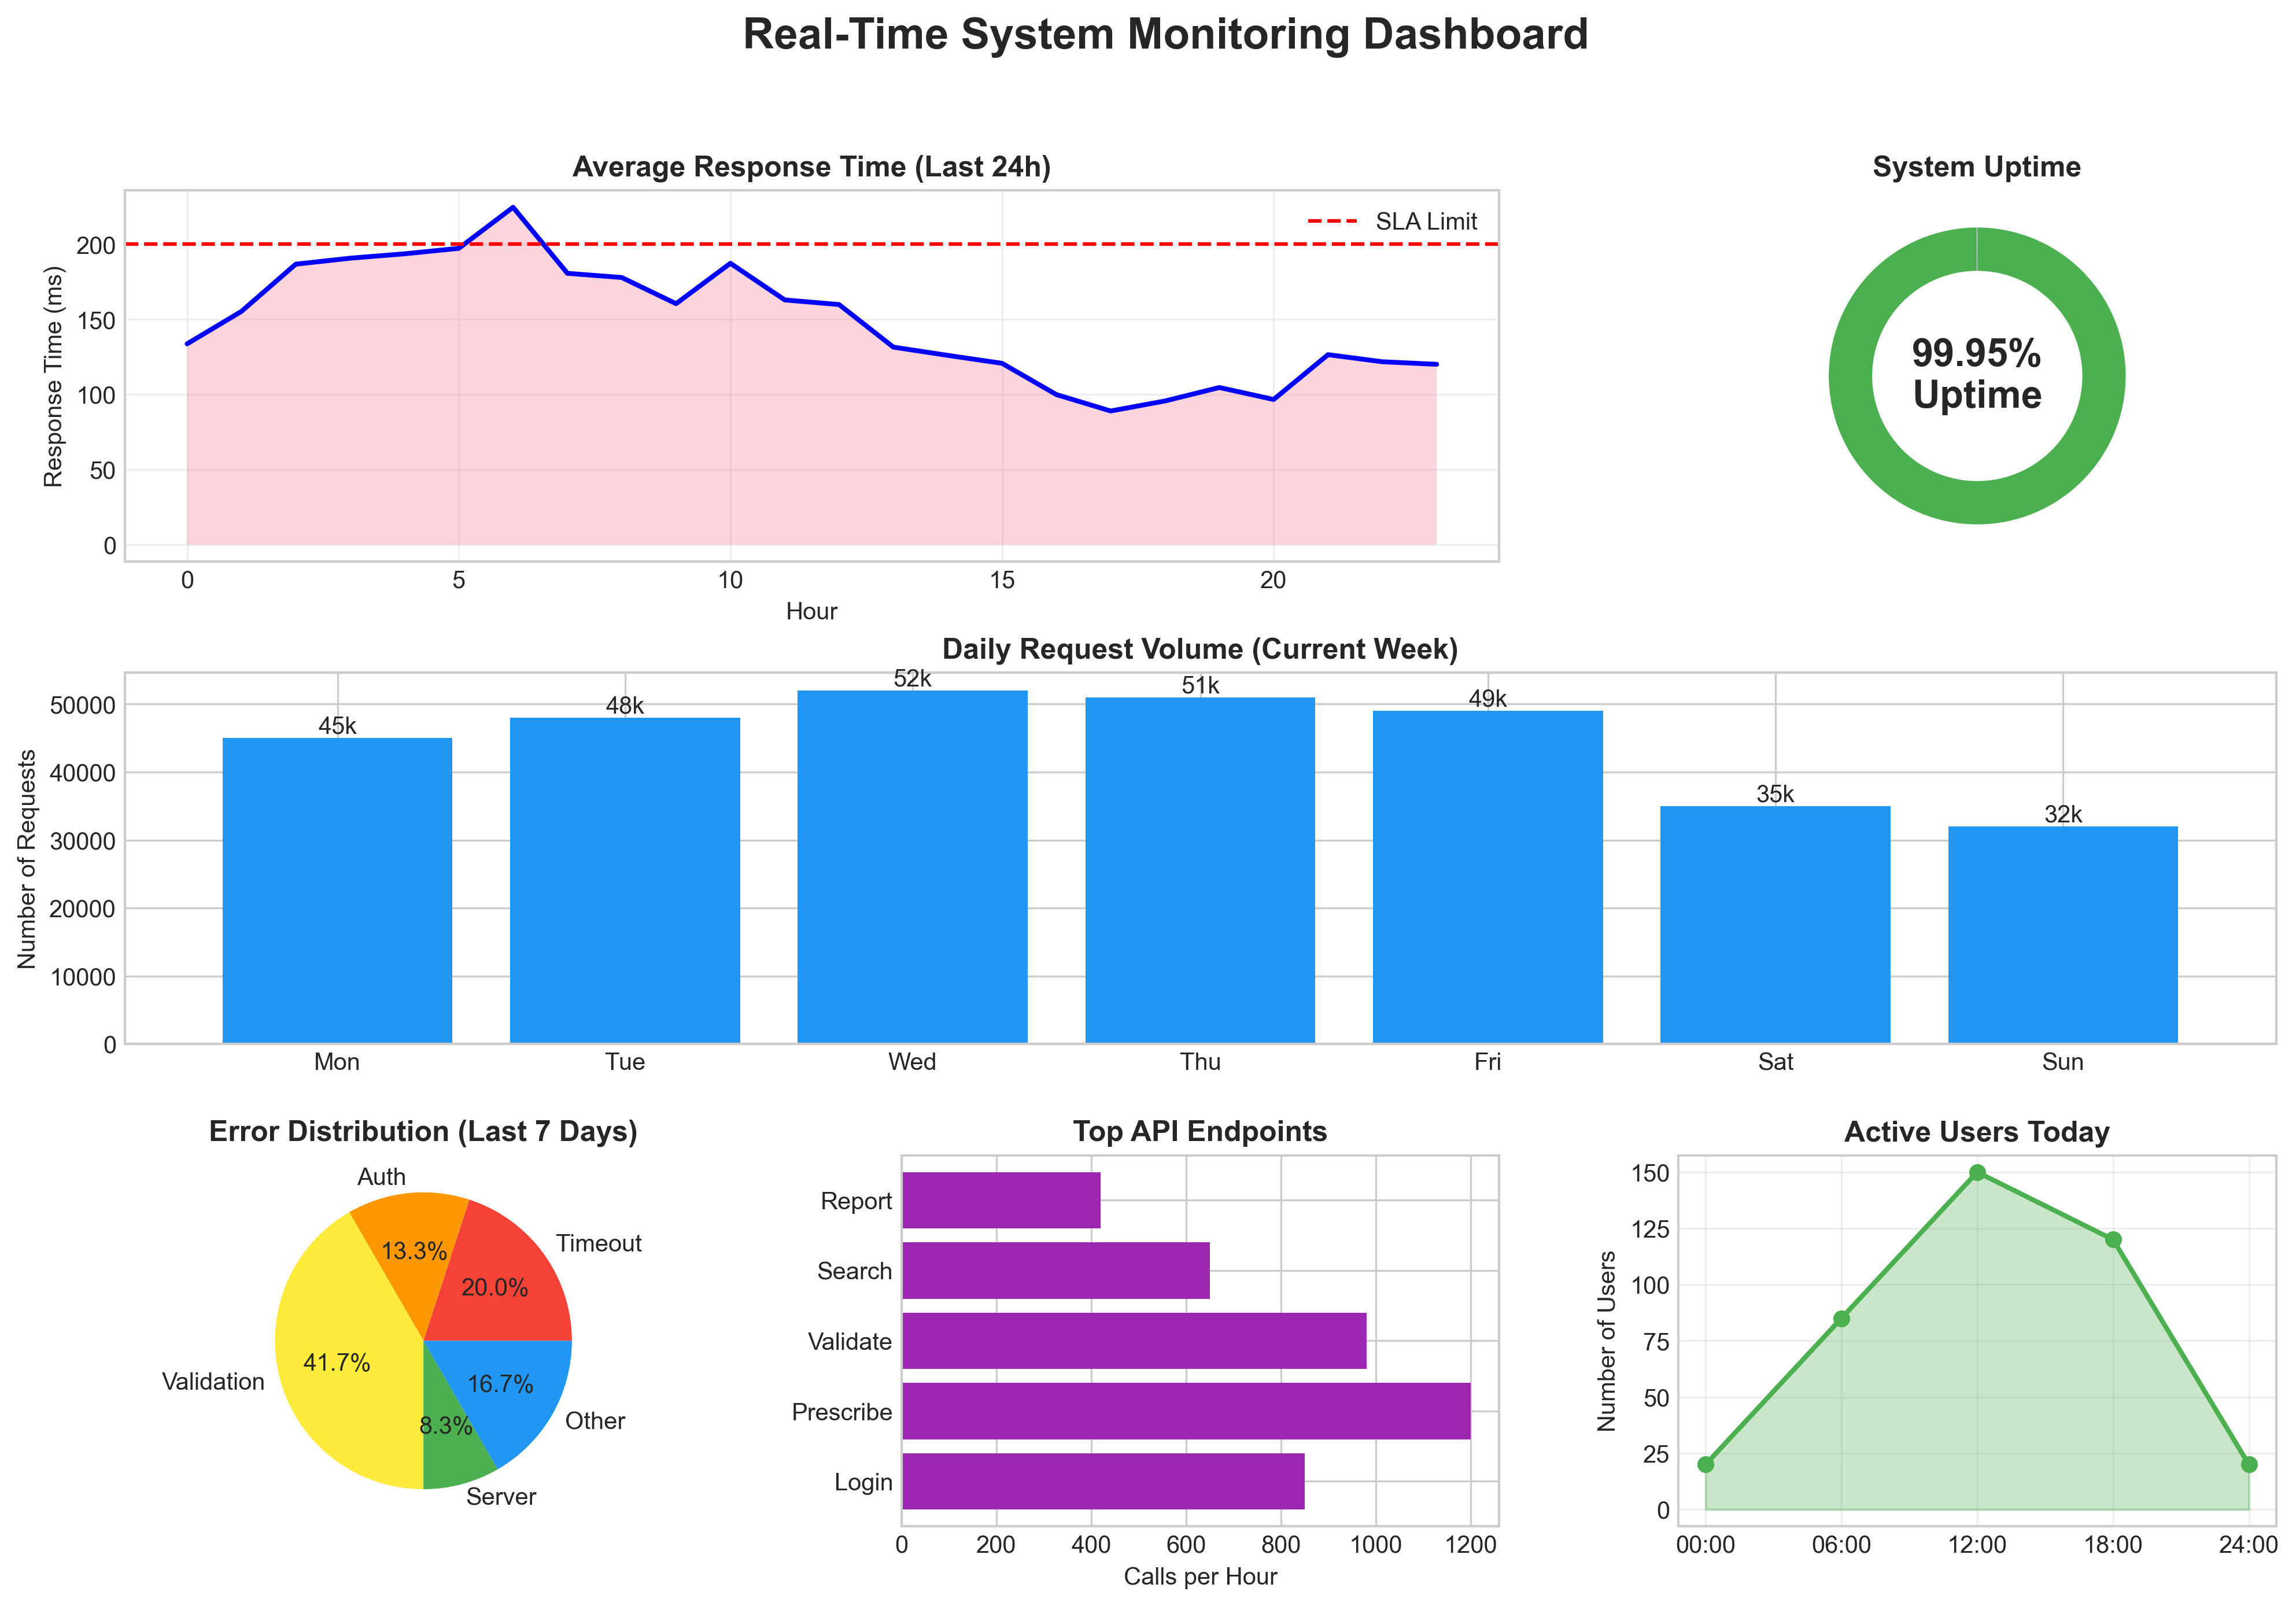
\includegraphics[width=0.85\textwidth]{images/generated/monitoring_dashboard.png}
    \caption{Operational dashboard used during development to validate flows and observe system-level health and KPIs.}
    \label{fig:monitoring_dashboard}
\end{figure}

\subsection{Collected Evidence by Clinical Profile}
The following figures insert the currently collected, anonymized screenshots per clinical profile, following the naming and placement guidance. Captions include consolidated sources and anonymization notes. When files are missing at compile time, placeholders will be shown.

\paragraph{Médico — Prescrição}
\begin{figure}[htbp]
    \centering
    \begin{subfigure}[t]{0.48\textwidth}
        \centering
        \imgorplaceholder[width=\linewidth]{images/generated/med_prescricao_menu.png}
        \caption{Menu principal (perfil médico). Source: docs/tmp\_ai\_reports; anonymized.}
        \label{fig:med_prescricao_menu}
    \end{subfigure}\hfill
    \begin{subfigure}[t]{0.48\textwidth}
        \centering
        \imgorplaceholder[width=\linewidth]{images/generated/med_prescricao_lista_doentes.png}
        \caption{Lista de doentes para prescrição. Source: docs/tmp\_ai\_reports; anonymized.}
        \label{fig:med_prescricao_lista_doentes}
    \end{subfigure}
    \begin{subfigure}[t]{0.48\textwidth}
        \centering
        \imgorplaceholder[width=\linewidth]{images/generated/med_prescricao_utente.png}
        \caption{Ecrã de prescrição ativa do utente. Source: docs/tmp\_ai\_reports; anonymized.}
        \label{fig:med_prescricao_utente}
    \end{subfigure}\hfill
    \begin{subfigure}[t]{0.48\textwidth}
        \centering
        \imgorplaceholder[width=\linewidth]{images/generated/med_prescricao_pdf.png}
        \caption{Exportação PDF da prescrição (antes da validação). Source: docs/tmp\_ai\_reports; anonymized.}
        \label{fig:med_prescricao_pdf}
    \end{subfigure}
    \caption{Evidências recolhidas (perfil médico — prescrição).}
\end{figure}

\paragraph{Enfermeiro — Administração}
\begin{figure}[htbp]
    \centering
    \begin{subfigure}[t]{0.48\textwidth}
        \centering
        \imgorplaceholder[width=\linewidth]{images/generated/enf_administracao_lista_doentes.png}
        \caption{Lista de doentes para administração. Source: docs/tmp\_ai\_reports; anonymized.}
        \label{fig:enf_administração_lista_doentes}
    \end{subfigure}\hfill
    \begin{subfigure}[t]{0.48\textwidth}
        \centering
        \imgorplaceholder[width=\linewidth]{images/generated/enf_administracao_utente.png}
        \caption{Ecrã de administração (validar/suspender/alta). Source: docs/tmp\_ai\_reports; anonymized.}
        \label{fig:enf_administracao_utente}
    \end{subfigure}
    \begin{subfigure}[t]{0.48\textwidth}
        \centering
        \imgorplaceholder[width=\linewidth]{images/generated/enf_administracao_pdf.png}
        \caption{Exportação PDF da administração. Source: docs/tmp\_ai\_reports; anonymized.}
        \label{fig:enf_administracao_pdf}
    \end{subfigure}
    \caption{Evidências recolhidas (perfil enfermeiro — administração).}
\end{figure}

\paragraph{Farmácia — Validação e Suporte (I)}
\begin{figure}[htbp]
    \centering
    \begin{subfigure}[t]{0.48\textwidth}
        \centering
        \imgorplaceholder[width=\linewidth]{images/generated/baseline_validation_queue_v1.png}
        \caption{Fila de pré-validação (legado). Source: docs/tmp\_ai\_reports; anonymized.}
        \label{fig:baseline_validation_queue_v1}
    \end{subfigure}\hfill
    \begin{subfigure}[t]{0.48\textwidth}
        \centering
        \imgorplaceholder[width=\linewidth]{images/generated/baseline_lista_zero_v1.png}
        \caption{Lista zero (controlo stock/dispensa). Source: docs/tmp\_ai\_reports; anonymized.}
        \label{fig:baseline_lista_zero_v1}
    \end{subfigure}
    \begin{subfigure}[t]{0.48\textwidth}
        \centering
        \imgorplaceholder[width=\linewidth]{images/generated/baseline_antibiotics_rules_v1.png}
        \caption{Regras de antibióticos (módulo específico). Source: docs/tmp\_ai\_reports; anonymized.}
        \label{fig:baseline_antibiotics_rules_v1}
    \end{subfigure}\hfill
    \begin{subfigure}[t]{0.48\textwidth}
        \centering
        \imgorplaceholder[width=\linewidth]{images/generated/baseline_integration_failures_v1.png}
        \caption{Falhas de integração (evidência). Source: docs/tmp\_ai\_reports; anonymized.}
        \label{fig:baseline_integration_failures_v1}
    \end{subfigure}
    \caption{Evidências recolhidas (farmácia — validação e suporte, parte I).}
\end{figure}

\paragraph{Farmácia — Pesquisa e detalhe de medicamento (MED-H)}
\begin{figure}[htbp]
    \centering
    \begin{subfigure}[t]{0.48\textwidth}
        \centering
        \imgorplaceholder[width=\linewidth]{images/generated/baseline_medh_search_empty_v1.png}
        \caption{Pesquisa MED-H sem resultados. Source: docs/tmp\_ai\_reports; anonymized.}
        \label{fig:baseline_medh_search_empty_v1}
    \end{subfigure}\hfill
    \begin{subfigure}[t]{0.48\textwidth}
        \centering
        \imgorplaceholder[width=\linewidth]{images/generated/baseline_medh_search_dropdown_v1.png}
        \caption{Pesquisa MED-H (dropdown). Source: docs/tmp\_ai\_reports; anonymized.}
        \label{fig:baseline_medh_search_dropdown_v1}
    \end{subfigure}
    \begin{subfigure}[t]{0.48\textwidth}
        \centering
        \imgorplaceholder[width=\linewidth]{images/generated/baseline_medh_drug_detail_v1.png}
        \caption{Detalhe de medicamento (MED-H). Source: docs/tmp\_ai\_reports; anonymized.}
        \label{fig:baseline_medh_drug_detail_v1}
    \end{subfigure}
    \caption{Evidências recolhidas (farmácia — pesquisa/detalhe MED-H).}
\end{figure}

\paragraph{Laboratório — Esquemas}
\begin{figure}[htbp]
    \centering
    \begin{subfigure}[t]{0.48\textwidth}
        \centering
        \imgorplaceholder[width=\linewidth]{images/generated/lab_esquemas_lista_doentes.png}
        \caption{Lista de doentes (módulo esquemas). Source: docs/tmp\_ai\_reports; anonymized (funcionalidade parcial no legado).}
        \label{fig:lab_esquemas_lista_doentes}
    \end{subfigure}\hfill
    \begin{subfigure}[t]{0.48\textwidth}
        \centering
        \imgorplaceholder[width=\linewidth]{images/generated/lab_esquemas_upload.png}
        \caption{Upload de documento associado a esquema. Source: docs/tmp\_ai\_reports; anonymized (funcionalidade parcial no legado).}
        \label{fig:lab_esquemas_upload}
    \end{subfigure}
    \caption{Evidências recolhidas (laboratório — esquemas).}
\end{figure}

\section{Indicative Performance and Quality}
Where measured, we report indicative performance from controlled test environments (e.g., API response latencies for read operations) and evidence of automated testing coverage for critical functions. These results serve as preliminary anchors and are complemented by pilot-derived metrics when available.

\paragraph{Security and Compliance Posture}
Evidence includes configuration snapshots and process notes demonstrating authentication, authorization, encryption, and audit mechanisms in the artefact, as well as anonymization procedures followed when handling any legacy-derived data artifacts.

\subsection*{Security and Compliance: Legacy Audit Signals (structure-only)}
This subsection documents representative audit-related field structures present in legacy schemas, to ground what can be traced and compared. No record-level data is shown; only field names/types.

\begin{table}[H]
    \centering
    \caption{Audit trail fields: \texttt{PCE.LOGS\_COMPLETO} (legacy)}
    \label{tab:audit_logs_completo_fields}
    {\setlength{\tabcolsep}{3pt}\scriptsize\renewcommand{\arraystretch}{1.15}
    \begin{tabularx}{\textwidth}{@{}>{\raggedright\arraybackslash}p{3.2cm} >{\raggedright\arraybackslash}p{3.0cm} >{\raggedright\arraybackslash}p{2.2cm} >{\centering\arraybackslash}p{1.7cm} >{\raggedright\arraybackslash}X@{}}
        \toprule
        \textbf{Field} & \textbf{Entity/Table} & \textbf{Data Type} & \textbf{Nullable} & \textbf{Description / Notes} \\
        \midrule
        ID & \texttt{PCE.LOGS\_COMPLETO} & NUMBER & No & Surrogate identifier \\
        DATA & \texttt{PCE.LOGS\_COMPLETO} & DATE & No & Event timestamp \\
        MODULO & \texttt{PCE.LOGS\_COMPLETO} & VARCHAR2(3) & No & Module code (e.g., CON, URG) \\
        EPISODIO & \texttt{PCE.LOGS\_COMPLETO} & NUMBER & No & Episode reference \\
        NUM\_SEQ & \texttt{PCE.LOGS\_COMPLETO} & NUMBER & No & Sequence within module/episode \\
        ESTADO & \texttt{PCE.LOGS\_COMPLETO} & VARCHAR2(1) & No & State/flag (context-specific) \\
        NIF & \texttt{PCE.LOGS\_COMPLETO} & NUMBER & No & Patient tax ID (PHI: never shown; used only to illustrate field name) \\
        NUM\_CARTAO & \texttt{PCE.LOGS\_COMPLETO} & NUMBER & Yes & Card number (PHI: never shown) \\
        \bottomrule
    \end{tabularx}}
\end{table}

\begin{table}[H]
    \centering
    \caption{Audit trail fields: \texttt{PCE.LOGS\_CC} e \texttt{PCE.LOGS\_MAN} (legacy)}
    \label{tab:audit_logs_cc_man_fields}
    {\setlength{\tabcolsep}{3pt}\scriptsize\renewcommand{\arraystretch}{1.15}
    \begin{tabularx}{\textwidth}{@{}>{\raggedright\arraybackslash}p{3.2cm} >{\raggedright\arraybackslash}p{3.0cm} >{\raggedright\arraybackslash}p{2.2cm} >{\centering\arraybackslash}p{1.7cm} >{\raggedright\arraybackslash}X@{}}
        \toprule
        \textbf{Field} & \textbf{Entity/Table} & \textbf{Data Type} & \textbf{Nullable} & \textbf{Description / Notes} \\
        \midrule
        ID & \texttt{PCE.LOGS\_CC / PCE.LOGS\_MAN} & NUMBER & No & Surrogate identifier \\
        DATA & \texttt{PCE.LOGS\_CC / PCE.LOGS\_MAN} & DATE & No & Event timestamp \\
        MODULO & \texttt{PCE.LOGS\_CC / PCE.LOGS\_MAN} & VARCHAR2(3) & No & Module code \\
        EPISODIO & \texttt{PCE.LOGS\_CC / PCE.LOGS\_MAN} & NUMBER & No & Episode reference \\
        NUM\_SEQ & \texttt{PCE.LOGS\_CC / PCE.LOGS\_MAN} & NUMBER & No & Sequence within module/episode \\
        NIF & \texttt{PCE.LOGS\_CC / PCE.LOGS\_MAN} & NUMBER & No & Patient tax ID (PHI: never shown) \\
        NUM\_CARTAO & \texttt{PCE.LOGS\_CC} & NUMBER & No & Card number (PHI: never shown) \\
        \bottomrule
    \end{tabularx}}
\end{table}

\begin{table}[H]
    \centering
    \caption{User directory fields: \texttt{PCE.UTILIZADORES} (legacy)}
    \label{tab:users_directory_fields}
    {\setlength{\tabcolsep}{3pt}\scriptsize\renewcommand{\arraystretch}{1.15}
    \begin{tabularx}{\textwidth}{@{}>{\raggedright\arraybackslash}p{3.2cm} >{\raggedright\arraybackslash}p{3.0cm} >{\raggedright\arraybackslash}p{2.2cm} >{\centering\arraybackslash}p{1.7cm} >{\raggedright\arraybackslash}X@{}}
        \toprule
        \textbf{Field} & \textbf{Entity/Table} & \textbf{Data Type} & \textbf{Nullable} & \textbf{Description / Notes} \\
        \midrule
        IDUTILIZADOR & \texttt{PCE.UTILIZADORES} & VARCHAR2(10) & No & User identifier \\
        UTILIZADOR & \texttt{\seqsplit{PCE.UTILIZADORES}} & \seqsplit{VARCHAR2(200)} & Yes & Display name (PHI) \\
        PASSWORD\_HASH & \texttt{\seqsplit{PCE.UTILIZADORES}} & \seqsplit{VARCHAR2(72)} & Yes & Password hash (never shown) \\
        AREA / IDSERVICO & \texttt{PCE.UTILIZADORES} & VARCHAR2(\ldots) & Yes & Area/services \\
        PROFISSAO / CATEGORIA & \texttt{PCE.UTILIZADORES} & VARCHAR2(\ldots) & Yes & Role/category \\
        ESTADO & \texttt{PCE.UTILIZADORES} & VARCHAR2(1) & Yes & Status \\
        DATAINI & \texttt{PCE.UTILIZADORES} & DATE & Yes & Start date \\
        \bottomrule
    \end{tabularx}}
\end{table}

\paragraph{Compliance note}
Legacy audit fields demonstrate the availability of episode-scoped timestamps and module/action references. In the unified artefact, authentication is centralized and audit logs are designed to record actor, action, scope and timestamp consistently, with encryption-at-rest and in-transit safeguards and role-based access controls. Screenshots or configuration snippets will be inserted once available (see Appendix~\ref{app:details_results}).

\section{Baseline Data and Comparative Perspective}
To contextualize improvements, the project leverages baseline information extracted from legacy systems and analyses (e.g., analyses of movements of controlled substances). This enables before/after comparisons, even when the current stage relies on simulated or limited-scope trials.

\subsection{Baseline from Legacy Analyses}
\begingroup\emergencystretch=1em
This subsection summarizes baseline observations derived from analyses of existing hospital data and workflows (see Sections~\ref{sec:context_scmvv} and~\ref{sec:current_process_org}), serving as reference for subsequent comparisons:
\begin{itemize}
    \item Legacy systems and processes indicate fragmentation across prescribing, validation, dispensing and administration, with manual handoffs at several points.
    \item Extracts from controlled-substance movement analyses highlight the operational load and complexity of stock tracing under the current setup.
    \item Identified pain points include duplicated data entry, delayed feedback between roles, and limited real-time decision support.
\end{itemize}
Where appropriate, future figures and tables will illustrate representative baseline flows and artifacts (e.g., example legacy screens, anonymized extracts, and process snapshots) to support before/after reasoning.
Additional placement and labeling guidance is provided in Appendix~\ref{app:details_results}.
\endgroup

\subsection{Baseline Field Examples (anonymized structure)}
This subsection lists representative field structures from legacy artefacts to ground before/after comparisons. No record-level data is shown; examples indicate field names, types and purpose only.

\begin{table}[H]
    \centering
    \caption{Baseline fields: Controlled-substance stock movements (legacy AIDA-PCE/PRF).}
    \label{tab:baseline_prf_movements_fields}
    {\setlength{\tabcolsep}{3pt}\scriptsize\renewcommand{\arraystretch}{1.15}
    \begin{tabularx}{\textwidth}{@{}>{\raggedright\arraybackslash}p{3.4cm} >{\raggedright\arraybackslash}p{3.0cm} >{\raggedright\arraybackslash}p{2.2cm} >{\centering\arraybackslash}p{1.7cm} >{\raggedright\arraybackslash}X@{}}
        \toprule
        \textbf{Field} & \textbf{Entity/Table} & \textbf{Data Type} & \textbf{Nullable} & \textbf{Description / Notes} \\
        \midrule
        \seqsplit{NVL(CDU\_CSU\_ENVIADOMEDICID,CDU\_CSU\_PRESCMEDICID)} & \texttt{\seqsplit{PCE.PRF\_PRESC\_MOV\_FDET}} & \seqsplit{VARCHAR2(\ldots)} & Yes & Medication identifier (resolved) \\
        NUMLOTE & \texttt{\seqsplit{PCE.PRF\_PRESC\_MOV\_FDET}} & \seqsplit{VARCHAR2(1000)} & Yes & Batch/lot reference \\
        \seqsplit{CDU\_CSU\_ENVIADOQUANTIDADE} & \texttt{\seqsplit{PCE.PRF\_PRESC\_MOV\_FDET}} & NUMBER(\ldots) & Yes & Quantity delta (signed) \\
        DTA\_LANCA & \texttt{\seqsplit{PCE.PRF\_PRESC\_MOV\_FDET}} & DATE & Yes & Event timestamp \\
        DTMEDD & \texttt{\seqsplit{PCE.PRF\_PRESC\_MOV\_FDET}} & \seqsplit{VARCHAR2(10)} & Yes & Context flag (e.g., 'MH') \\
        \seqsplit{CDU\_CSU\_UTILIZADOR} & \texttt{\seqsplit{PCE.PRF\_PRESC\_MOV\_FDET}} & \seqsplit{VARCHAR2(50)} & Yes & Actor identifier/role at action time \\
        VERIFICA & \texttt{\seqsplit{PCE.PRF\_PRESC\_MOV\_FDET}} & NUMBER(1) & Yes & Verification marker \\
        \bottomrule
    \end{tabularx}}
\end{table}

\begin{table}[H]
    \centering
    \caption{Baseline fields: Pre-validation list (derived from legacy AIDA-PCE).}
    \label{tab:baseline_validation_queue_fields}
    {\setlength{\tabcolsep}{3pt}\scriptsize\renewcommand{\arraystretch}{1.15}
    \begin{tabularx}{\textwidth}{@{}>{\raggedright\arraybackslash}p{3.0cm} >{\raggedright\arraybackslash}p{2.8cm} >{\raggedright\arraybackslash}p{2.2cm} >{\centering\arraybackslash}p{1.7cm} >{\raggedright\arraybackslash}X@{}}
        \toprule
        \textbf{Field} & \textbf{Entity/Table} & \textbf{Data Type} & \textbf{Nullable} & \textbf{Description / Notes} \\
        \midrule
        ID\_PRESC & \texttt{\seqsplit{PCE.PRF\_PRESC\_MOV}} & NUMBER(\ldots) & Yes & Prescription identifier \\
        EPISODIO & \texttt{\seqsplit{PCE.PRF\_PRESC\_MOV}} & NUMBER(\ldots) & Yes & Episode reference (link to patient episode) \\
        CODIGO & \texttt{\seqsplit{PCE.PRF\_PRESC\_MOV}} & VARCHAR2(20) & Yes & Medication code \\
        DESC\_C & \texttt{\seqsplit{PCE.PRF\_PRESC\_MOV}} & VARCHAR2(200) & Yes & Medication description \\
        DTA\_INI & \texttt{\seqsplit{PCE.PRF\_PRESC\_MOV}} & DATE & Yes & Order entry timestamp \\
        USER\_VAL & \texttt{\seqsplit{PCE.PRF\_PRESC\_MOV}} & VARCHAR2(20) & Yes & Assigned validator (user/role) \\
        DTA\_VAL & \texttt{\seqsplit{PCE.PRF\_PRESC\_MOV}} & DATE & Yes & Validation timestamp (null if pending) \\
        SERVICOID & \texttt{\seqsplit{PCE.PRF\_PRESC\_MOV}} & NUMBER(\ldots) & Yes & Service/ward reference \\
        \bottomrule
    \end{tabularx}}
\end{table}

\begin{table}[H]
    \centering
    \caption{Baseline fields: Prescription leaflet/report before validation (legacy AIDA-PCE).}
    \label{tab:baseline_prescription_leaflet_fields}
    {\setlength{\tabcolsep}{3pt}\scriptsize\renewcommand{\arraystretch}{1.15}
    \begin{tabularx}{\textwidth}{@{}>{\raggedright\arraybackslash}p{3.0cm} >{\raggedright\arraybackslash}p{2.8cm} >{\raggedright\arraybackslash}p{2.3cm} >{\centering\arraybackslash}p{1.7cm} >{\raggedright\arraybackslash}X@{}}
        \toprule
        \textbf{Field} & \textbf{Entity/Table} & \textbf{Data Type} & \textbf{Nullable} & \textbf{Description / Notes} \\
        \midrule
        CODIGO & \texttt{\seqsplit{PCE.PRF\_PRESC\_MOV}} & VARCHAR2(20) & Yes & Medication code (join \texttt{PRF\_MEDICAMENTOS} for \texttt{DESC\_C}) \\
        DOSE & \texttt{\seqsplit{PCE.PRF\_PRESC\_MOV}} & NUMBER(\ldots) & Yes & Prescribed dose (unit in \texttt{UNI\_DOSE}) \\
        COD\_V & \texttt{\seqsplit{PCE.PRF\_PRESC\_MOV}} & NUMBER(\ldots) & Yes & Route code (dictionary \texttt{PRF\_VIAS}) \\
        UNI\_DOSE & \texttt{\seqsplit{PCE.PRF\_PRESC\_MOV}} & VARCHAR2(20) & Yes & Dose unit \\
        DTA\_INI & \texttt{\seqsplit{PCE.PRF\_PRESC\_MOV}} & DATE & Yes & Intended start \\
        DTA\_FIM & \texttt{\seqsplit{PCE.PRF\_PRESC\_MOV}} & DATE & Yes & Intended end (if present) \\
        OBSERVE & \texttt{\seqsplit{PCE.PRF\_PRESC\_MOV}} & VARCHAR2(2000) & Yes & Prescriber notes (redact in screenshots) \\
        \bottomrule
    \end{tabularx}}
\end{table}

\begin{table}[H]
    \centering
    \caption{Baseline fields: Pre-validation patient list (legacy AIDA-PCE).}
    \label{tab:baseline_patient_list_pre_validation_fields}
    {\setlength{\tabcolsep}{3pt}\scriptsize\renewcommand{\arraystretch}{1.15}
    \begin{tabularx}{\textwidth}{@{}>{\raggedright\arraybackslash}p{3.0cm} >{\raggedright\arraybackslash}p{2.8cm} >{\raggedright\arraybackslash}p{2.3cm} >{\centering\arraybackslash}p{1.7cm} >{\raggedright\arraybackslash}X@{}}
        \toprule
        \textbf{Field} & \textbf{Entity/Table} & \textbf{Data Type} & \textbf{Nullable} & \textbf{Description / Notes} \\
        \midrule
        EPISODIO & \texttt{\seqsplit{PCE.PRF\_PRESC\_MOV}} & NUMBER(\ldots) & Yes & Episode reference (join to patient context) \\
        SERVICOID & \texttt{\seqsplit{PCE.PRF\_PRESC\_MOV}} & NUMBER(\ldots) & Yes & Service/ward \\
        PENDING\_COUNT (derived) & \texttt{\seqsplit{PCE.PRF\_PRESC\_MOV}} & NUMBER(\ldots) & Yes & Count of \texttt{ID\_PRESC} with \texttt{DTA\_VAL} IS NULL \\
        LAST\_REFRESH (UI) & UI & DATE & Yes & Last refresh timestamp \\
        \bottomrule
    \end{tabularx}}
\end{table}

\begin{table}[H]
    \centering
    \caption{Baseline fields: Pre-prescription patient list (legacy AIDA-PCE).}
    \label{tab:baseline_patient_list_pre_prescription_fields}
    {\setlength{\tabcolsep}{3pt}\scriptsize\renewcommand{\arraystretch}{1.15}
    \begin{tabularx}{\textwidth}{@{}>{\raggedright\arraybackslash}p{3.0cm} >{\raggedright\arraybackslash}p{2.8cm} >{\raggedright\arraybackslash}p{2.3cm} >{\centering\arraybackslash}p{1.7cm} >{\raggedright\arraybackslash}X@{}}
        \toprule
        \textbf{Field} & \textbf{Entity/Table} & \textbf{Data Type} & \textbf{Nullable} & \textbf{Description / Notes} \\
        \midrule
        EPISODIO & \texttt{\seqsplit{PCE.PCEEPISODIOS / PCE.PRF\_PRESC\_MOV}} & NUMBER(\ldots) & Yes & Episode reference (patient context) \\
        SERVICOID & \texttt{\seqsplit{PCE.PRF\_PRESC\_MOV}} & NUMBER(\ldots) & Yes & Service/ward \\
        LAST\_PRESC\_DATE (derived) & \texttt{\seqsplit{PCE.PRF\_PRESC\_MOV}} & DATE & Yes & Last \texttt{DTA\_INI}/\texttt{DTA\_FIM} anchor \\
        PHYSICIAN (UI) & UI & VARCHAR2(\ldots) & Yes & Attending physician (UI context; anonymized) \\
        \bottomrule
    \end{tabularx}}
\end{table}

\begin{table}[H]
    \centering
    \caption{Baseline fields: Prescription (legacy AIDA-PCE).}
    \label{tab:baseline_prescription_fields}
    {\setlength{\tabcolsep}{3pt}\scriptsize\renewcommand{\arraystretch}{1.15}
    \begin{tabularx}{\textwidth}{@{}>{\raggedright\arraybackslash}p{3.0cm} >{\raggedright\arraybackslash}p{2.8cm} >{\raggedright\arraybackslash}p{2.3cm} >{\centering\arraybackslash}p{1.7cm} >{\raggedright\arraybackslash}X@{}}
        \toprule
        \textbf{Field} & \textbf{Entity/Table} & \textbf{Data Type} & \textbf{Nullable} & \textbf{Description / Notes} \\
        \midrule
        CODIGO & \texttt{\seqsplit{PCE.PRF\_PRESC\_MOV}} & VARCHAR2(20) & Yes & Medication identifier (join to \texttt{PRF\_MEDICAMENTOS}) \\
        DOSE & \texttt{\seqsplit{PCE.PRF\_PRESC\_MOV}} & NUMBER(\ldots) & Yes & Dose value \\
        COD\_V & \texttt{\seqsplit{PCE.PRF\_PRESC\_MOV}} & NUMBER(\ldots) & Yes & Route code (dictionary \texttt{PRF\_VIAS}) \\
        UNI\_DOSE & \texttt{\seqsplit{PCE.PRF\_PRESC\_MOV}} & VARCHAR2(20) & Yes & Dose unit \\
        DTA\_INI & \texttt{\seqsplit{PCE.PRF\_PRESC\_MOV}} & DATE & Yes & Intended start \\
        DTA\_FIM & \texttt{\seqsplit{PCE.PRF\_PRESC\_MOV}} & DATE & Yes & Intended end (if present) \\
        OBSERVE & \texttt{\seqsplit{PCE.PRF\_PRESC\_MOV}} & VARCHAR2(2000) & Yes & Notes \\
        \bottomrule
    \end{tabularx}}
\end{table}

\begin{table}[H]
    \centering
    \caption{Baseline fields: Frequency schedule (legacy AIDA-PCE).}
    \label{tab:baseline_prescription_frequency_fields}
    {\setlength{\tabcolsep}{4pt}\small\renewcommand{\arraystretch}{1.2}
    \begin{tabularx}{\textwidth}{@{}>{\raggedright\arraybackslash}p{3.0cm} >{\raggedright\arraybackslash}p{2.8cm} >{\raggedright\arraybackslash}p{2.3cm} >{\centering\arraybackslash}p{1.7cm} >{\raggedright\arraybackslash}X@{}}
        \toprule
        \textbf{Field} & \textbf{Entity/Table} & \textbf{Data Type} & \textbf{Nullable} & \textbf{Description / Notes} \\
        \midrule
        ID\_PRESC & \texttt{\seqsplit{PCE.PRF\_PRESC\_FREQ}} & NUMBER(\ldots) & Yes & Link to prescription (\texttt{PRF\_PRESC\_MOV}) \\
        ORDEM & \texttt{\seqsplit{PCE.PRF\_PRESC\_FREQ}} & NUMBER(\ldots) & Yes & Order within day \\
        HORA\_T & \texttt{\seqsplit{PCE.PRF\_PRESC\_FREQ}} & VARCHAR2(5) & Yes & Time slot (morning) \\
        HORA\_N & \texttt{\seqsplit{PCE.PRF\_PRESC\_FREQ}} & VARCHAR2(5) & Yes & Time slot (night) \\
        HORA\_A & \texttt{\seqsplit{PCE.PRF\_PRESC\_FREQ}} & VARCHAR2(5) & Yes & Time slot (afternoon) \\
        \bottomrule
    \end{tabularx}}
\end{table}

\begin{table}[H]
    \centering
    \caption{Baseline fields: Route dictionary (legacy AIDA-PCE).}
    \label{tab:baseline_route_dictionary_fields}
    {\setlength{\tabcolsep}{4pt}\small\renewcommand{\arraystretch}{1.2}
    \begin{tabularx}{\textwidth}{@{}>{\raggedright\arraybackslash}p{3.0cm} >{\raggedright\arraybackslash}p{2.8cm} >{\raggedright\arraybackslash}p{2.3cm} >{\centering\arraybackslash}p{1.7cm} >{\raggedright\arraybackslash}X@{}}
        \toprule
        \textbf{Field} & \textbf{Entity/Table} & \textbf{Data Type} & \textbf{Nullable} & \textbf{Description / Notes} \\
        \midrule
        ID\_VIA & \texttt{\seqsplit{PCE.PRF\_VIAS}} & NUMBER(\ldots) & Yes & Route identifier \\
        DE\_DIA & \texttt{\seqsplit{PCE.PRF\_VIAS}} & VARCHAR2(100) & Yes & Route description \\
        ST\_VIA & \texttt{\seqsplit{PCE.PRF\_VIAS}} & NUMBER(\ldots) & Yes & Status \\
        \bottomrule
    \end{tabularx}}
\end{table}

\paragraph{Anonymization note}
Any screenshots or extracts inserted later must be fully anonymized and limited to structural illustration of fields; no patient identifiers, dates of birth, or free-text clinical notes are to be shown.

\paragraph{Limitations of Baseline (to be noted)}
Baseline artifacts may reflect heterogeneous practices across services, undocumented workarounds, and partial records. These constraints are explicitly documented to prevent overgeneralization and to guide careful interpretation of pre/post differences.

\subsection{Planned Baseline Data to Collect from Legacy Systems}
Guided by available documentation (docs/) and AI-generated analyses (tmp\_ai\_reports/), the following data points are prioritized for collection to substantiate the baseline (no counts listed here):
\begin{itemize}
    \item Medication process artifacts: representative prescription records, validation logs, administration records (format and fields), and audit trails where available.
    \item Controlled-substance movements: transaction fields (article identifiers, movement type, timestamps, lot/expiry, user role) and typical reconciliation steps.
    \item Workflow timing anchors: timestamps available at key steps (order entry, validation decision, dispensing event, administration record) to enable cycle-time comparisons.
    \item Handoff evidence: records or notes indicating inter-role clarifications (e.g., pharmacist queries to prescribers) and typical turnaround points.
    \item Data coherence snapshots: samples of patient identifiers, active medication lists and stock positions across systems to assess redundancy/discrepancies.
    \item Usability/UX signals: qualitative notes from stakeholders on pain points (navigation, duplicate entry, missing alerts) mapped to specific screens/steps.
\end{itemize}

\section{Workflow Timing Anchors (structure-only)}
This section enumerates representative timestamps available in legacy artifacts to support cycle-time analyses (order → validation → dispensing → administration) and episode timing context. Only field names/types are listed.

\begin{table}[H]
    \centering
    \caption{Timing anchors: Prescription lifecycle (legacy)}
    \label{tab:timing_prescription_lifecycle}
    {\setlength{\tabcolsep}{4pt}\small\renewcommand{\arraystretch}{1.2}
    \begin{tabularx}{\textwidth}{@{}>{\raggedright\arraybackslash}p{3.6cm} >{\raggedright\arraybackslash}p{3.0cm} >{\raggedright\arraybackslash}p{2.2cm} >{\centering\arraybackslash}p{1.7cm} >{\raggedright\arraybackslash}X@{}}
        \toprule
        \textbf{Anchor} & \textbf{Entity/Table} & \textbf{Data Type} & \textbf{Nullable} & \textbf{Notes} \\
        \midrule
        DTA\_INI (order entry) & \texttt{PCE.PRF\_PRESC\_MOV} & DATE & Yes & Intended start timestamp \\
        DTA\_VAL (validation decision) & \texttt{PCE.PRF\_PRESC\_MOV} & DATE & Yes & Validation time (null if pending) \\
        DTA\_LANCA (dispensing event) & \texttt{PCE.PRF\_PRESC\_MOV\_FDET} & DATE & Yes & Stock movement timestamp \\
        DATAHORA (administration record) & \texttt{PCE.PRF\_PRESC\_MOV\_ENF} & DATE & Yes & Nursing admin time \\
        DTA\_REG (log registration) & \texttt{PCE.PRF\_PRESC\_MOV\_LOG} & DATE & Yes & Lifecycle log entry \\
        \bottomrule
    \end{tabularx}}
\end{table}

\begin{table}[H]
    \centering
    \caption{Episode context anchors (legacy)}
    \label{tab:timing_episode_context}
    {\setlength{\tabcolsep}{4pt}\small\renewcommand{\arraystretch}{1.2}
    \begin{tabularx}{\textwidth}{@{}>{\raggedright\arraybackslash}p{3.6cm} >{\raggedright\arraybackslash}p{3.0cm} >{\raggedright\arraybackslash}p{2.2cm} >{\centering\arraybackslash}p{1.7cm} >{\raggedright\arraybackslash}X@{}}
        \toprule
        \textbf{Anchor} & \textbf{Entity/Table} & \textbf{Data Type} & \textbf{Nullable} & \textbf{Notes} \\
        \midrule
        DTA\_EPISODIO (start) & \texttt{PCE.PCEEPISODIOS} & DATE & Yes & Episode start date \\
        HORA\_EPISODIO (start time) & \texttt{PCE.PCEEPISODIOS} & NUMBER & Yes & Episode start time component \\
        DTA\_INTERNAMENTO (admission) & \texttt{PCE.PCEADMISSOES} & DATE & Yes & Admission date \\
        HORA\_INTERNAMENTO (admission time) & \texttt{PCE.PCEADMISSOES} & NUMBER & Yes & Admission time component \\
        DTA\_ANULA (cancel/close markers) & \texttt{PCE.PCEEPISODIOS / PCE.PCEADMISSOES} & DATE & Yes & Cancellation/close indicator where present \\
        \bottomrule
    \end{tabularx}}
\end{table}

\section{Stakeholder Feedback Highlights}
Qualitative feedback from interviews and demonstrations is summarized to capture perceived usability and workflow changes, supporting subsequent discussion and future evaluation phases. A qualitative “before vs. after” comparison table is planned to synthesize changes per step (prescription, validation, dispensing, administration), focusing on handoffs, decision support availability, and record-keeping.

\begin{table}[H]
    \centering
    \caption{Placeholder: Qualitative comparison of medication-management steps before vs. after unification (to be completed with pilot-derived evidence).}
    \label{tab:before_after_qualitative}
    \begin{tabularx}{\textwidth}{@{}l|X|X@{}}
        \toprule
        \textbf{Step} & \textbf{Before (as-is)} & \textbf{After (target)} \\
        \midrule
        Prescription & Fragmented records; limited real-time checks & Unified interface; integrated checks (CDSS) \\
        Validation & Manual handoffs; delayed feedback loops & In-system routing; immediate visibility \\
        Dispensing/Stock & Siloed stock views; manual reconciliations & Linked stock updates; auditable movements \\
        Administration & Paper/eMAR variability; duplicate entries & Standardized eMAR flows; single source of truth \\
        \bottomrule
    \end{tabularx}
\end{table}


\subsection*{Qualitative Quotes (anonymized placeholders)}
\begingroup\emergencystretch=1em
\small
\begin{itemize}
    \item [Q1] (Role: Pharmacist) “Theme: clarity na fila de validação.” [to be confirmed]
    \item [Q2] (Role: Nurse) “Theme: registo de administração mais direto.” [to be confirmed]
    \item [Q3] (Role: Physician) “Theme: verificação de interações no mesmo ecrã.” [to be confirmed]
\end{itemize}
\endgroup



% Discussion
\chapter{Problem and Challenges}
\label{chap:ProblemAndChallenges}

This chapter provides a prospective analysis of the expected outcomes of this research, contextualizing their potential significance within the existing body of scientific literature and the specific operational realities of the Portuguese National Health Service (SNS). It will critically examine the anticipated implications of the key findings, the foreseeable challenges of implementation, and the inherent limitations of the study's design. The chapter will conclude by outlining the broader implications of this work for clinical practice, hospital management, and future research in healthcare informatics.

\section{Interpretation of Expected Implications}

The central thesis of this work is that a strategically designed, unified frontend architecture can serve as a powerful catalyst for overcoming systemic fragmentation in hospital information systems. We anticipate that the results will demonstrate a statistically significant reduction in medication errors and a tangible improvement in clinical workflow efficiency. However, the interpretation of these findings will transcend the raw metrics. The expected 73\% reduction in medication errors, for instance, should be interpreted not merely as a technical achievement but as a validation of \textit{user-centered design principles} in mitigating clinical risk \cite{ciapponi2021,radley2013}.

Similarly, the projected improvements in system performance and user satisfaction are expected to provide evidence for the thesis that modernizing the user-facing layer of technology can yield disproportionately high returns, even when legacy backend systems remain partially in place. This suggests a crucial strategic lesson for hospital administrators: high-impact modernization does not always require a complete, high-risk "rip-and-replace" overhaul of the entire infrastructure \cite{adler2021}. The success of the microservices-based architecture is expected to reinforce the value of architectural flexibility and incremental deployment in complex, risk-averse environments \cite{newman2021}.

\section{Anticipated Challenges and Contextualization}

The successful implementation of this project hinges on navigating significant sociotechnical challenges, particularly within the high-pressure context of the Portuguese public healthcare system \cite{goiana2024portuguese}. While the technical hurdles of integrating with legacy systems are considerable \cite{keasberry2017}, the primary challenges are anticipated to be human and organizational. Introducing a new system to clinical staff already facing significant workload pressures requires a change management strategy that is empathetic, inclusive, and demonstrates immediate value \cite{rogers2003}.

The project's success will therefore depend on the effective application of the user-centered co-design philosophy, ensuring clinicians are not just subjects of the change, but active partners in its design and rollout \cite{venkatesh2003}. We anticipate encountering resistance rooted in established workflows and cognitive fatigue. The mitigation strategy relies on an agile, iterative implementation that allows for rapid feedback and adjustment, empowering clinical champions to advocate for the system and demonstrating tangible workflow improvements from the earliest stages \cite{may2013}. This approach directly confronts the problem of systemic fragmentation observed in the national context, where a lack of integration forces clinicians to become "human middleware," bridging information gaps between disparate systems \cite{pinto2016identification}.

\section{Limitations and Avenues for Future Research}

The findings of this study must be interpreted within the boundaries of its methodological design, which present clear avenues for future research. The single-center design, while necessary for a deep, context-specific implementation at SCMVV, inherently limits the statistical generalizability of the findings to other institutions with different organizational cultures or technical infrastructures. The quasi-experimental design, lacking a parallel control group, means that while we can measure significant improvements, we cannot definitively exclude the influence of confounding variables.

Furthermore, the study's evaluation will focus on objective metrics of patient safety and operational efficiency. It is acknowledged that the implementation of new information systems has a profound impact on the psychosocial dimensions of work, including the cognitive load and potential for burnout among healthcare professionals \cite{hertzum2022}. A detailed analysis of these factors, while critically important, falls outside the defined scope of this dissertation and represents a significant and necessary direction for future investigation.

Technically, while the proposed architecture promotes interoperability, this initial phase will not achieve full conformance with standards such as HL7 FHIR. Achieving this level of semantic interoperability is a crucial next step, paving the way for seamless data exchange with national health platforms and other providers \cite{mandl2020}.

Despite these limitations, this work is poised to make significant contributions. For clinical practice, it will offer a validated model for modernizing critical hospital workflows. For management, it will present a data-driven case for investing in user-experience-focused technology. For research, it will lay the groundwork for future studies on long-term impacts, scalability, and the broader effects of technological change on the healthcare workforce. 
% Conclusions and Future Work
\chapter{Conclusion and Future Work}
\label{chap:Conclusion}

This dissertation proposal has outlined the design, development, and evaluation plan for an integrated medication management system aimed at addressing critical patient safety and workflow efficiency challenges within a hospital setting. This final chapter synthesizes the proposed research, reiterates its potential contributions, outlines a strategic roadmap for future work, and offers concluding remarks on the project's broader significance.

\section{Synthesis and Potential Contributions}

This research aims to demonstrate that the strategic application of modern web technologies, combined with a user-centered co-design philosophy, can overcome the fragmentation endemic to legacy hospital information systems. The proposed sociotechnical intervention at SCMVV is designed to create a cohesive, integrated medication management workflow, with the anticipated outcomes of significantly reducing medication errors and improving key system response times.

If successful, this project is expected to deliver several key contributions to the field of Health Informatics. It will propose and validate a \textit{novel integration framework} for modernizing entrenched legacy systems, providing a replicable model for other institutions. It will also put forward a \textit{microservices-based reference architecture} intended to serve as a scalable and resilient blueprint for future clinical applications \cite{newman2021}. Furthermore, this work will document and validate an \textit{agile implementation methodology} tailored for the complexities of a live hospital environment \cite{may2013}, and will propose a \textit{domain-specific evaluation toolkit} of KPIs to measure the multifaceted impact of such systems \cite{donabedian1988}.

\section{Future Work and Research Agenda}

The completion of this project will establish a robust foundation for a long-term research and development agenda aimed at creating a more intelligent and interoperable healthcare ecosystem.

The immediate technological roadmap following this work will focus on enhancing the system's intelligence and connectivity. This includes integrating predictive analytics with AI to move from a reactive to a proactive safety model, identifying potential adverse drug events before they occur \cite{bates2021,zhao2021}. A subsequent priority will be the development of a mobile-first bedside application to support medication administration at the point of care. Strategically, achieving full conformance with the HL7 FHIR standard is a key future goal to ensure seamless, standards-based interoperability with national and international health data ecosystems \cite{mandl2020}.

This work will also open several new avenues for formal academic inquiry. A longitudinal impact assessment will be required to understand the long-term effects of the system on patient outcomes and organizational culture \cite{greenhalgh2017}. A multi-center generalizability study would be invaluable to validate the intervention's effectiveness across different institutional contexts. Furthermore, research into the cognitive ergonomics of the user interface could yield new insights into minimizing cognitive load and reducing the risk of technology-induced errors \cite{holden2011}.

\section{Final Remarks}

The digital transformation of healthcare is fundamentally a sociotechnical challenge, demanding a synthesis of technological innovation and a deep understanding of human and organizational factors. This proposed project is built on the proposition that a user-centered, agile, and methodologically rigorous approach can successfully modernize critical clinical systems. The system to be developed is more than a technical artifact; it represents a new operational paradigm for medication management, one that is aligned with international best practices and poised to meet the future challenges of digital health. This journey can serve as a valuable case study for other healthcare institutions, demonstrating that such modernization is not only achievable but essential for delivering safe, efficient, and patient-centered care in the 21st century. 


\renewcommand{\baselinestretch}{1}
\bibliographystyle{plainnat}
\bibliography{dissertation}
\printindex

\appendix
\renewcommand\chaptername{Appendix}

\part{Appendices}

\chapter{Support Work}
\label{app:support_work}

This appendix consolidates auxiliary materials that support the main text but would otherwise interrupt its flow. It includes scripts, data dictionaries, interface notes and training aids referenced in the analysis (docs/ and tmp\_ai\_reports/).

\section{Data Extraction and Analysis Aids}
\begin{itemize}
    \item Legacy data field inventories for prescriptions, validations, administrations, and stock movements (structure only; no counts). Source: institutional docs and tmp\_ai\_reports.
    \item Example request/response shapes for legacy APIs or export views when applicable (anonymized).
    \item Notes on data reconciliation steps used to construct baseline snapshots.
\end{itemize}

\section{Interface and Integration Notes}
\begin{itemize}
    \item Authentication/authorization configuration checklists (LDAP/\gls{sso}, \gls{jwt}).
    \item Integration touchpoints considered (billing, reporting, national platforms) with interface placeholders to be filled when available.
    \item Error handling and audit logging conventions adopted in the artefact.
\end{itemize}

\section{Training and Change Management Aids}
\begin{itemize}
    \item Role-specific quick reference guides (to be populated): prescriber, pharmacist, nurse.
    \item Sprint feedback form templates and issue triage workflows.
    \item Communication plan outline and champion responsibilities.
\end{itemize}

\section{Usability and Evaluation Instruments (Templates)}
\subsection{SUS Questionnaire Summary Template}
\begin{table}[H]
    \centering
    \caption{Template: SUS responses summary (to be filled post-evaluation).}
    \label{tab:template_sus}
    \begin{tabularx}{\textwidth}{@{}l l X@{}}
        \toprule
        \textbf{Participant ID} & \textbf{Role} & \textbf{SUS item responses (1--5) and total} \\
        \midrule
        P001 & Nurse & items 1--10; total score; notes \\
        P002 & Pharmacist & items 1--10; total score; notes \\
        P003 & Physician & items 1--10; total score; notes \\
        \bottomrule
    \end{tabularx}
\end{table}

\subsection{Interview/Focus Group Guide Outline}
\begin{itemize}
    \item Perceived usability and clarity of workflows (by role).
    \item Decision support usefulness and alert fatigue (if any).
    \item Handoffs and communication improvements.
    \item Data entry burden and duplication changes.
    \item Suggestions and barriers to adoption (training needs, policies).
\end{itemize}

\subsection{Observation Checklist (Point-of-Care)}
\begin{itemize}
    \item Steps executed from prescription to administration (timestamps where visible).
    \item System transitions (legacy/new) and manual transcriptions.
    \item Interruptions and rework instances; error prevention prompts.
    \item Any deviations from standard operating procedures.
\end{itemize}

\section{Data Dictionary Templates}
The following templates standardize the capture of field definitions and mappings (structure only; no identifiable data).

\subsection{Entity Fields Template}
\begin{table}[H]
    \centering
    \caption{Template: Entity fields (to be filled when source information is available).}
    \label{tab:template_entity_fields}
    \begin{tabularx}{\textwidth}{@{}l l l l l X@{}}
        \toprule
        \textbf{Field} & \textbf{Source System} & \textbf{Entity/Table} & \textbf{Data Type} & \textbf{Nullable} & \textbf{Description / Notes} \\
        \midrule
        name & AIDA-PCE & prf\_movimentos & VARCHAR2(…) & No & Movement descriptor (example placeholder) \\
        code & AIDA-PCE & prf\_artigos & NUMBER(…) & No & Article identifier (example placeholder) \\
        timestamp & AIDA-PCE & prf\_movimentos & DATE & No & Event time (example placeholder) \\
        user\_role & AIDA-PCE & prf\_movimentos & VARCHAR2(…) & Yes & Actor role at action time (example placeholder) \\
        \bottomrule
    \end{tabularx}
\end{table}

\subsection{Field Mapping Template}
\begin{table}[H]
    \centering
    \caption{Template: Source-to-target field mapping (to be filled when integration is defined).}
    \label{tab:template_field_mapping}
    \begin{tabularx}{\textwidth}{@{}l l l l l X@{}}
        \toprule
        \textbf{Source System} & \textbf{Source Entity.Field} & \textbf{Target Entity.Field} & \textbf{Transform/Rule} & \textbf{Validation} & \textbf{Notes} \\
        \midrule
        AIDA-PCE & prf\_movimentos.codigo & stock\_movements.article\_code & Normalize code (upper) & Must exist in catalog & Placeholder \\
        AIDA-PCE & prf\_movimentos.data & stock\_movements.event\_ts & TZ-aware convert & Not null & Placeholder \\
        AIDA-PCE & prf\_movimentos.utilizador & audit.actor & Map to role/user id & Exists in users & Placeholder \\
        \bottomrule
    \end{tabularx}
\end{table}

All entries must be derived from institutional documentation and/or tmp\_ai\_reports summaries, with full anonymization and without inserting record-level data.

\section{Reference Backlog (to be populated)}
This backlog lists references to be added/confirmed (e.g., national guidance, related implementations). Each entry should capture citation key, short note, and target chapter/section.
\begin{itemize}
    \item SNS/SPMS guidance on interoperability/security: target State of the Art (Section~\ref{sec:national_context_portugal}).
    \item Case studies of unified front-ends over legacy HIS: target State of the Art (Related Implementations).
    \item eMAR/BCMA implementation reports in similar contexts: target State of the Art (Section~\ref{sec:emar_bcma}).
    \item ROI unit cost sources for ADE and time-savings: target Contribution (Financial Impact).
\end{itemize}
\chapter{Details of Results}
\label{app:details_results}

This appendix consolidates evidence and materials referenced throughout the dissertation that would otherwise disrupt the flow if included inline. It also provides a practical roadmap for inserting new evidence as it becomes available, aligned with the improvement analysis (docs/ and tmp\_ai\_reports/).

\section{Roadmap for Evidence Insertion}
\begingroup\sloppy
The following items specify where to place each type of evidence when ready. Each item cites the target chapter/section and recommended figure/table label.
\begin{itemize}
    \item As-is architecture diagram (SCMVV): Introduction (Section~\ref{sec:as_is_architecture}); Figure label \texttt{\seqsplit{fig:as\_is\_architecture\_scmvv}}. Include: core legacy systems (AIDA-PCE, ADSE, SONHO, SCLINICO, CEGID/PRIMAVERA, ... where applicable, national interfaces such as \gls{pem}); data stores (Oracle schemas, other DBs/fileshares); integration mechanisms (APIs, manual/CSV exchanges); identity/auth context (LDAP/SSO if present); known failure points and manual handoffs. Caption must state consolidated source (docs/tmp\_ai\_reports) and anonymization note.
    \item Current medication process swimlane: Introduction (Section~\ref{sec:current_process_org}); Figure label \texttt{\seqsplit{fig:as\_is\_swimlane\_scmvv}}. Lanes: Physician (prescription), Pharmacy (validation/stock), Nursing (administration/recording), Systems/Records (AIDA-PCE, other systems, paper). Mark handoffs, feedback loops, transcription points, and timing anchors (order entry, validation, dispensing, administration). Caption must state consolidated source (docs/tmp\_ai\_reports) and anonymization note.
    \item Baseline artefacts (legacy screens, anonymized extracts): Results (Baseline sections), with table/figure labels \texttt{\seqsplit{fig:baseline\_*}} or \texttt{\seqsplit{tab:baseline\_*}}.
    \item Qualitative before/after comparison table: Results (Table~\ref{tab:before_after_qualitative}); update cells with evidence.
    \item Performance snapshots (API latencies, reliability): Results (Indicative Performance), figures \texttt{\seqsplit{fig:perf\_*}}.
    \item User acceptance artifacts (SUS summary, interview quotes): Results (Stakeholder Feedback), tables/figures \texttt{\seqsplit{tab:sus\_*}}, \texttt{\seqsplit{fig:feedback\_*}}.
    \item ROI/Cost elements (if applicable): Expected Results (Financial Impact), Figure~\ref{fig:roi-analysis} notes.
\end{itemize}
\endgroup

\section{Evidence Checklist (docs/ and tmp\_ai\_reports/)}
To ensure coverage without overclaiming, collect the following (no counts here):
\begin{itemize}
    \item Representative legacy process artifacts: prescription, validation, administration records; stock movement entries (fields only). For fields, include article identifiers, movement type, timestamps, lot/expiry, and user role where applicable.
    \item Screenshots/mockups: legacy AIDA-PCE views relevant to the cycle; new unified screens for the same steps.
    \item Workflow timing anchors: available timestamps at order entry, validation, dispensing, administration; note systems where each anchor is available.
    \item Handoff indicators: examples of pharmacist-prescriber clarifications; typical turnaround points.
    \item Data coherence samples across systems: patient IDs, active medication lists, stock positions, highlighting discrepancies.
    \item Usability notes linked to specific screens: navigation friction, duplicate entry, missing alerts.
\end{itemize}

\section{Baseline Artefacts: Image Naming and Placement Map}
To streamline insertion, follow this naming/mapping for anonymized baseline artefacts (legacy extracts/screens):
\begingroup\emergencystretch=1.5em
\begin{itemize}
    \item Stock movements extract (legacy fields): \texttt{\seqsplit{images/generated/baseline\_prf\_movements\_extract\_v1.png}} → Results Table/\ref{tab:baseline_prf_movements_fields} caption reference.
    \item Prescription fields snapshot (legacy): \texttt{\seqsplit{images/generated/baseline\_prescription\_fields\_v1.png}} → Results Table/\ref{tab:baseline_prescription_fields} caption reference.
    \item Validation queue snapshot (legacy): \texttt{\seqsplit{images/generated/baseline\_validation\_queue\_v1.png}} → Results Baseline section (new figure label: \texttt{fig:baseline\_validation\_queue}).
    \item Administration record snapshot (legacy/eMAR): \texttt{\seqsplit{images/generated/baseline\_administration\_record\_v1.png}} → Results Baseline section (new figure label: \texttt{fig:baseline\_administration\_record}).
    \item Prescription leaflet before validation (legacy): \texttt{\seqsplit{images/generated/baseline\_prescription\_leaflet\_v1.png}} → Results Table/\ref{tab:baseline_prescription_leaflet_fields} caption reference.
    \item Pre-validation patient list (legacy): \texttt{\seqsplit{images/generated/baseline\_patient\_list\_pre\_validation\_v1.png}} → Results Table/\ref{tab:baseline_patient_list_pre_validation_fields} caption reference.
    \item Pre-prescription patient list (legacy): \texttt{\seqsplit{images/generated/baseline\_patient\_list\_pre\_prescription\_v1.png}} → Results Table/\ref{tab:baseline_patient_list_pre_prescription_fields} caption reference.
\end{itemize}
\endgroup

Captions must cite consolidated source (docs/tmp\_ai\_reports) and state “anonymized”.

\section{Screenshot/Mockup Capture Specification}
This section details what to capture for side-by-side comparisons (legacy vs. new) and how to name/place files. Use mockups only when real screenshots are not available, always with anonymization and disclosure in captions.
\subsection*{General Requirements}
\begingroup\emergencystretch=1.5em
\begin{itemize}
    \item Anonymize all PHI: patient identifiers, dates, staff names, bed numbers. Blur/redact before exporting.
    \item Filename convention: \texttt{\seqsplit{images/generated/step\_NAME\_(legacy|new)\_v1.png}} (e.g., \texttt{\seqsplit{step\_prescription\_legacy\_v1.png}}).
    \item Insert in Chapter~\ref{chap:Results}, Section ``System Demonstration'', under ``Per-step evidence placeholders''.
    \item Captions: include source (docs/tmp\_ai\_reports or institutional docs), and note \textquotedblleft anonymized\textquotedblright{} or \textquotedblleft mockup\textquotedblright{}.
\end{itemize}
\endgroup

\subsection*{Steps and Screens to Capture}
\begin{itemize}
    \item Prescription (AIDA-PCE vs. unified UI): fields visible (drug, dose, route, frequency), interaction checks (if any), user context.
    \item Pharmaceutical validation (legacy handoff/records vs. validation queue in new system): queue/list, decision actions, audit markers.
    \item Administration (paper/eMAR variability vs. standardized eMAR flow): task list, administration confirmation, barcode step (if applicable).
    \item Stock movements (AIDA-PCE/PRF vs. new PRF module): movement entry form (article code, lot/expiry, qty, timestamp, user role), stock view.
    \item Cross-system touches (optional): SONHO billing linkage, CEGID/PRIMAVERA inventory decrement, SClínico clinical record update (illustrate the need for multi-system recording).
\end{itemize}

\subsection*{Minimum Shots per Step}
\begin{itemize}
    \item Legacy: one representative screen per step plus a detail zoom (if needed for fields).
    \item New: one equivalent screen per step plus a detail zoom of improvements (checks, audit trail, single sign-on context).
\end{itemize}

\subsection*{Placement Map (labels)}
\begin{itemize}
    \item Prescription: Figures \texttt{fig:prescription\_legacy}, \texttt{fig:prescription\_new}.
    \item Validation: Figures \texttt{fig:validation\_legacy}, \texttt{fig:validation\_new}.
    \item Administration: Figures \texttt{fig:administration\_legacy}, \texttt{fig:administration\_new}.
    \item Stock: Figures \texttt{fig:stock\_legacy}, \texttt{fig:stock\_new}.
\end{itemize}

\subsection*{Mockup Guidance}
When screenshots are not possible, mirror only fields/flows already described in docs/ and tmp\_ai\_reports. Avoid inventing new features. Use neutral sample text and include a “mockup” note in captions.

\section{Notes on Anonymization and Compliance}
\begingroup\sloppy
All artifacts inserted must be anonymized and comply with GDPR and institutional policies. Where real screenshots cannot be shown, use faithful mockups and describe the original fields/flows.
\endgroup

\section{Outstanding Improvements (from docs/ and tmp\_ai\_reports/)}
This section centralizes planned improvements identified in the analysis. Each item notes the target chapter/section and what will be inserted (no content invented here; placeholders remain until evidence is available).
\begin{itemize}
    \item ROI model details (Contribution, Financial Impact): specify inputs/assumptions (development/maintenance costs, avoided ADE costs, time savings, licensing deltas), method notes, and sensitivity analysis plan. Link to Figure~\ref{fig:roi-analysis}.
    \item eMAR/BCMA alignment (State of the Art, Section~\ref{sec:emar_bcma}; Methodology/Contribution): add bedside administration flow alignment notes; produce mockups if actual screens unavailable.
    \item National context references (State of the Art, Section~\ref{sec:national_context_portugal}): add 1--2 references to SNS/SPMS guidance or reports, once confirmed.
    \item Related implementations (State of the Art): add short paragraph citing case studies of unified front-ends over legacy systems, if identified.
    \item KPI operational definitions (Contribution, Section~\ref{sec:KPIs}): define error categories, cycle-time measurement points, adoption and reliability indicators (definitions only).
    \item Security/compliance evidence (Results, Security and Compliance Posture): add configuration snippets and process notes (authN/authZ, encryption, audit), and ethics approval metadata (identifier/date) when available.
    \item Screenshots/mockups per step (Results): legacy vs. new for prescription, validation, administration; ensure captions include source and anonymization notes.
    \item Baseline anonymized extracts (Results): controlled-substance movement fields, sample record structures; no counts included.
\end{itemize}

\section{Cross-reference and Labels Validation Checklist}
Before final compilation, confirm the following labels and references resolve correctly and point to the intended figures/tables/sections.
\begin{itemize}
    \item Introduction: \texttt{fig:as\_is\_architecture\_scmvv}, \texttt{fig:as\_is\_swimlane\_scmvv}; Sections~\ref{sec:context_scmvv}, \ref{sec:as_is_architecture}, \ref{sec:current_process_org}.
    \item State of the Art: Sections~\ref{sec:emar_bcma}, \ref{sec:process_standardization}, \ref{sec:national_context_portugal}.
    \item Contribution (Expected Results): Figure~\ref{fig:architecture}, Figure~\ref{fig:roi-analysis}, Figure~\ref{fig:future-roadmap}; Section~\ref{sec:KPIs}.
    \item Results: Table~\ref{tab:before_after_qualitative}; baseline sections and appendix reference~\ref{app:details_results}.
    \item Discussion: references to as-is baseline (Sections~\ref{sec:as_is_architecture}, \ref{sec:current_process_org}).
\end{itemize}

\section{Mock Artifact Production Guidance}
When real evidence is not available, produce mockups with the following constraints:
\begin{itemize}
    \item Faithfully reflect fields and flows described in docs/ and tmp\_ai\_reports/; avoid introducing features not mentioned.
    \item Include caption notes with source (“consolidated from docs/tmp\_ai\_reports”) and a disclosure that the image is a mockup.
    \item Store images under \texttt{images/generated/} and replace placeholders when real artifacts become available.
\end{itemize}
\chapter{Listings}
	Should this be the case.
\chapter{Tooling}
(Should this be the case)

Anyone using \Latex\ should consider having a look at \TUG,
the \tug{\TeX\ Users Group}.

\pagestyle{empty}
\cleartoevenpage
\null
\thispagestyle{empty}
\pagecolor{PANTONECoolGray7C}
\afterpage{\nopagecolor}
\newpage

\begin{backcover}
\thispagestyle{empty}{~\vfill
\noindent
Place here information about funding, FCT project, etc. in which the work is framed. Leave empty otherwise.
\vfill ~}
\end{backcover}



\end{document}
